%----------------------------------------------------------------------------------------------------------------------
% \documentclass[a4paper,10pt]{report}  % class article, amsart, report, IEEEtran, etc
%\documentclass[journal]{IEEEtran}
\documentclass[mscres,ianc,logo,twoside,deptreport]{infthesis} %deptreport,singlespacing,abbreviations
%-----------------------------------   start of generic preamble -----------------------------------
%
% \usepackage{geometry}         % See geometry.pdf to learn the layout options. There are lots.
% \geometry{a4paper}            % letterpaper or a4paper or a5paper or ... 
% \geometry{landscape}          % Activate for rotated page geometry
% \usepackage[parfill]{parskip} % Activate to begin paragraphs with an empty line rather than an indent
%
% \usepackage{multicol}         % For n-column layout
% These things may be useful when using multicol:
% \usepackage{calc}             % allows raisebox, can more baselines
% \usepackage{stfloats}         % page-wide floats at h or b as well as t
% \usepackage{fixltx2e}         % number-ordering with page-wide floats
%
%
%%%%% For making PDFs with eps graphics
%
% it's different for making dvis!
\usepackage[pdftex]{graphicx}
%
\usepackage{epstopdf}
% on command line, call with:
%--shell-escape --enable-write18
%
\DeclareGraphicsRule{.tif}{png}{.png}{`convert #1 `dirname #1`/`basename #1 .tif`.png}
%\epstopdfsetup{suffix=-\SourceExt-converted-to}
%
\usepackage{grffile}                    % allow dots in middle of filenames
%
%
%%%%% Math Styling Packages
\usepackage{amssymb,amstext,amsmath}    % full math equation support
\usepackage{amsfonts}                   % for blackboard bold, etc
\usepackage{amsthm}                     % better theorem environments
%
%
%%%%% General Packages
%\usepackage{mathtools}              % includes the ability to put text over => arrows
%... Alternatively, can use \stackrel
%\usepackage[tight]{subfigure}       % ability to place figures side-by-side %need to swap to subfig sometime!
% \usepackage{subfig}                 % the new version of subfigure (not backward compatible)
% \usepackage{caption}
% \usepackage{subcaption}              % the even newer version of subfigure (not backward compatible)
\usepackage{hyperref}               % hyperlinks references and citations
\usepackage{placeins}               % adds \FloatBarrier
\usepackage[super,nospace]{cite}    % superscript citations. NB: sort,compress on by default.
%
%
%%%%% Table packages
%
\usepackage{multirow}               % items can span multiple table rows/cols
%
\usepackage{booktabs}               % professional quality tables
% see http://ctan.mackichan.com/macros/latex/contrib/booktabs/booktabs.pdf
%
\usepackage{dcolumn}                % lets you align decimal points
\newcolumntype{d}[1]{D{.}{.}{#1}}   % Adds decimal point column type. Must specify the number of decimal places as arg.
%
% \usepackage{ctable}                % for different table captions in the text/footnotes/list of tables (uses booktabs)
%
% \usepackage{longtable}             % for tables spanning multiple pages
%
%
%%%%% Quoting Code
% \usepackage{color}                % use if color is used in text
\usepackage{verbatim}               % useful for program listings
% \usepackage{listings}             % also useful for program listings (use lstlisting environment)
% \lstset{language=Python}          % set params for listings
\usepackage[numbered]{mcode}        % for including matlab code
% mcode info at http://my.opera.com/locksley90/blog/2008/02/25/how-to-include-matlab-source-code-in-a-latex-document
% http://www.mathworks.com/matlabcentral/fileexchange/8015/
%
%
%%%%% Various Theorems etc (numbered by chapter)
% \theoremstyle{plain}% default
% \newtheorem{thm}{Theorem}%[chapter]
% \newtheorem*{thm*}{Theorem}               %un-numbered
% \newtheorem{lem}[thm]{Lemma}
% \newtheorem{prop}[thm]{Proposition}
% \newtheorem{cor}[thm]{Corollary}
% %
% \theoremstyle{definition}
% \newtheorem{defn}[thm]{Definition}
% \newtheorem{conj}[thm]{Conjecture}
% \newtheorem{exmp}[thm]{Example}
% %
% \theoremstyle{remark}
% \newtheorem*{rem}{Remark}
% \newtheorem*{note}{Note}
% \newtheorem{case}{Case}[chapter]
%
%
%%%%% Math notation
%
% These curly letters can be useful for making unique math symbols
\DeclareMathAlphabet{\mathpzc}{OT1}{pzc}{m}{it}
% use this in body with just \mathpzc{H} etc
%
%
%%% Operators
%
% Derivatives
\let\underdot=\d                                        % rename builtin command \d{} to \underdot{}
%\renewcommand{\d}{\operatorname{d}}                     % old method
\renewcommand{\d}{\ensuremath{\operatorname{d}\!}}      % straight operator d (\! for no space after)
%\renewcommand{\d}{\ensuremath{d}}                       % italic (variable-like) d
\newcommand{\od}[1]{\frac{\d}{\d#1}}                    % first order ordinary derivative operator
\newcommand{\odn}[2]{\frac{\d^{#2}}{\d#1^{#2}}}         % n-th order ordinary derivative operator
\newcommand{\pd}[1]{\frac{\partial}{\partial #1}}       % first order partial derivative operator
\newcommand{\pdn}[2]{\frac{\partial^{#2}}{\partial #1^{#2}}}    % n-th order partial derivative operator
%
%%% `Log-like' functions
\DeclareMathOperator{\sgn}{sgn}                         % sign
\DeclareMathOperator*{\E}{\mathop{\mathbb E\/}}         % expectation
%
%
%%% Ordinals
%\newcommand{\ord}[2]{#1#2}                              %where we are doing normal 1st, 2nd, 3rd, 4th and not n-th
\newcommand{\ord}[2]{\ensuremath{\text{#1}^\text{#2}}}  %where we are doing normal 1st, 2nd, 3rd, 4th and not n-th
%\newcommand{\nth}[1]{#1\text{-th}}                      %where the argument is mathematical and we are in math-mode
%\newcommand{\mth}[1]{$#1$-th}                           %where the argument is mathematical but we are not in math-mode
\newcommand{\nth}[1]{\ensuremath{#1\text{-th}}}         %NEW: where argument is mathematical (may be used in any mode)
\newcommand{\mth}[1]{\nth{#1}}                          %ditto. for backward compatibility.
%
%%% Vectors
\newcommand{\mtx}[1]{\left[ \begin{matrix} #1 \end{matrix} \right]} %matrix
\newcommand{\col}[1]{\mtx{#1}}                                      %column vector
\newcommand{\row}[1]{[#1]}                                          %row vector
\newcommand{\tcol}[1]{\row{#1}^T}                                   %transposed col vector
%
%%% Notation
\newcommand{\VEC}[1]{\mathbf{#1}}                                   %vector symbol typeface
\newcommand{\SET}[1]{\mathbf{#1}}                                   %set symbol typeface
\newcommand{\NSYS}[1]{\mathbb{#1}}                                  %number system typeface (R, C, Z, N)
%
%
%%%%% Homebrew commands (to save typing)
%
% Text
%\newcommand{\ie}{i.e. }
%\newcommand{\eg}{e.g. }
%
%
%-----------------------------------   end of generic preamble -----------------------------------
%
%-----------------------------------   start of file-specific preamble -----------------------------------
%
%
% \usepackage[numbers,sort&compress]{natbib}
% \usepackage{natmove} % moves superscript references after the punctuation mark regardless of where \cite command appears
% \usepackage{hypernat}
% \bibpunct{}{}{,}{s}{}{} % superscript citation
%
%
\usepackage{caption}
\usepackage{subcaption}              % the even newer version of subfigure (not backward compatible)
\renewcommand{\thesubfigure}{\Alph{subfigure}}
%
\captionsetup{margin=.5cm,indention=.2cm,labelsep=period}
\captionsetup[subfigure]{singlelinecheck=off,labelformat=simple,labelfont=bf}
%
% http://www.tug.org/texlive/Contents/live/texmf-dist/doc/latex/units/units.pdf
\usepackage{nicefrac}                % nice fractions
\usepackage{units}                   % nice units
%
\newcommand{\etal}{\textit{et al.}}
\newcommand{\eg}{\textit{e.g.}}
\newcommand{\ie}{\textit{i.e.}}
\newcommand{\NB}{{N.B.}}
%
\newcommand{\R}{\NSYS{R}}                                           %number system typeface (R, C, Z, N)
\newcommand{\C}{\NSYS{C}}                                           %number system typeface (R, C, Z, N)
\newcommand{\Z}{\NSYS{Z}}                                           %number system typeface (R, C, Z, N)
\newcommand{\N}{\NSYS{N}}                                           %number system typeface (R, C, Z, N)
% 
\makeatletter
\def\cleartoevenpage{\clearpage\if@twoside \ifodd\c@page
    \hbox{}\newpage\if@twocolumn\hbox{}\newpage\fi\fi\fi}
\makeatother
%
\usepackage[perpage,symbol*,splitrule]{footmisc}
\interfootnotelinepenalty=10000                                     % no carrying on to next page
%
%-----------------------------------   end of file-specific preamble -----------------------------------
%
%----------------------------------------------------------------------------------------------------------------------
%
%
\title{An information theoretic analysis of perceptual learning data from macaque V1 and V4}
\author{Scott~Lowe}
\abstract{%
A three month project applying information theoretic techniques to a dataset of spiking activity collected from Multi-Electrode Arrays in visual cortex regions V1 and V4, for two macaque monkeys is described.
We consider how the mutual information between the spiking activity patterns of individual neurons and the contrast of the presented stimulus changes with learning.
In particular, a spike timing neural code is compared to a spike count code, and it is found that the spike timing code only offers more information during the onset transient response, and this is additional information does not change with learning.
The effects of perceptual learning on coarse and fine contrast discrimination is also explored within the information theoretic framework, and it is found that there is no increase information in the spike-trains of individual neurons for either fine or coarse discrimination for V1, and in V4 there is an increase only for coarse discrimination.
For coarse discrimination in V4, the results also indicate there is a decrease in the latency of information, which we believe to be an entirely novel result, though current work only finds this in one of the two monkeys in the study.
Along the way, several problems inherent to the dataset had to be overcome, and a novel method of removing periodic artifacts from spiking data is proposed and utilised.
}
%
%
\begin{document}
%
%% First, the preliminary pages
\begin{preliminary}
%
%% This creates the title page
\maketitle
%
%
%% Acknowledgements
\begin{acknowledgements}
Thanks to the Engineering and Physical Sciences Research Council (EPSRC), Medical Research Council (MRC) and Biotechnology and Biological Sciences Research Council (BBSRC) for providing funding which supported me throughout this project.

Thanks to Xing Chen, for collecting and making available all the data analysed in this report.
% Given the amount of data which must be collected for a perceptual learning study, this is certainly a significant undertaking.

Thanks to Prof. Stefano Panzeri, for collaborating on the project, offering pertinent advice on how proceed with several aspects of the information theoretic analysis, and casting his eye on the preliminary results.

Thanks to Prof. Alex Thiele, for taking a very active and helpful role in supervision throughout this project.
\end{acknowledgements}
%
%
%% Next we need to have the declaration.
\standarddeclaration
%
%% Finally, a dedication (this is optional -- uncomment the following line if
%% you want one).
% \dedication{To my mummy.}
%
%% Create the table of contents
\tableofcontents
%
%% If you want a list of figures or tables, uncomment the appropriate line(s)
% \listoffigures
% \listoftables
%
\end{preliminary}
%
%
%%%%%%%%
%% Include your chapter files here. See the sample chapter file for the basic
%% format.
%
%----------------------------------------------------------------------------------------------------------------------
\section{Introduction}

In this study, we will be examining how the ability of individual neurons to discriminate between multiple stimuli changes over many exposures to the stimuli.
This will be done by means of an information theoretic analysis of the experimentally collected data.
To begin, we will consider some background material to give the reader a feel for the field.

%----------------------------------------------------------------------------------------------------------------------
%----------------------------------------------------------------------------------------------------------------------
\subsection{Background}
\label{ch:bg}

To the best of the author's knowledge, surprisingly, no previous study to date has analysed perceptual learning in an information theoretic framework.
Consequently in this section we will offer the reader an overview in both perceptual learning and information theory in isolation from one another.

%----------------------------------------------------------------------------------------------------------------------
\subsubsection{Perceptual Learning}
\label{sec:bgpl}

When an individual repeatedly performs a sensory perception task they will typically demonstrate an improvement in performance. If the task is repeated until performance reaches saturation, the effect can persist for months. This phenomenon is known as perceptual learning, and its duration sets it apart from shorter term effects such as sensitization (transient increase in sensitivity following a period of stimulation) and priming (change in perception of one stimulus immediately following a different, faint, stimulus).
Tasks well suited to studying perceptual learning involve making fine distinctions between different sensory inputs, such as discerning between lines of similar orientations.

It has been noted that improvements in perception are highly specific to the task at hand. For example, for visual tasks perceptual learning has no effect on performance if the stimulus is displaced by as little as $3^\circ$ in the visual field from the training location \cite{Gilbert1994}, 
and a vernier acuity task on the separation of lines has no transfer to the same task with dots \cite{Poggio1992}.

% extend, more examples, cited

Psychologists and psychophysicists have long known that it is possible for training to improve performance on discrimination tasks across a variety of sensory modalities, such as visual acuity, somatosensory spatial resolution, hue discrimination, estimation of weight and discrimination of pitch \cite{Gilbert2001}; but the fact that it occurs for such a low-level tasks is still surprising to the uninitiated. More specific examples of perceptual learning in the visual system include discrimination of differences in the offset of two lines, discrimination of orientation of lines, discrimination of direction of motion, and perception of depth in random-dot stereograms \cite{Gilbert2001,Fine2002}.

There is still some contention over where the physiological changes which lead to perceptual learning are situated in the brain. Consequently, there are several competing models which attempt to explain how perceptual learning arises.
The `early' model hypothesises that improvements principally occur at a low level in the sensory cortex \cite{Gilbert2001,Fahle2005}.
The `late' model states that improvements are in higher level cortical areas related to decision making \cite{Yu2004}.
Whilst according to the `reverse hierarchy model', improvements are made first in higher level decision areas, and then these are propagated down the cortical hierarchy to lower levels via top-down feedback signals if the changes at higher levels are insufficient \cite{Ahissar2004,Hochstein2002}.

Perceptual learning is thought to be connected to cortical remapping and reorganisation in response to similar stimuli \cite{Dinse2003,Pleger2003,Polley2006}. In such experiments, the region of the cortex coding for the stimulus is seen to expand.
Some researchers in this field have suggested that perceptual learning might be the mechanism which underpins all adult plasticity in the sensory and association cortices \cite{Gilbert2001}.


Neural changes correlated with perceptual learning have been observed at many levels of the cortical hierarchy. Studies have found changes in the orientation tuning curves of neurons in both V1 \cite{Schoups2001} and V4 \cite{Yang2004,Raiguel2006}, however the effects are greater in V4 than in V1 \cite{Raiguel2006}, and not all studies find neural changes in V1 and V2 which relate to perceptual learning, even when the subject has demonstrated psychometric improvement in the task \cite{Ghose2002}.

Due to the specificity of perceptual learning, only neurons in the retinotopic area where the stimulus falls are affected. 
When the properties of individual neurons have been observed to change during perceptual learning, their tuning curves for task-relevant features have become sharper (\ie{} the bandwidth narrows). Under activity-based models of neural information processing, this will provide more information about the task-relevant stimulus property if it falls on the steeper slope of the tuning curve. Studies have also shown that the effect of perceptual learning is most pronounced on the most relevant neurons from the perspective of information conveyed \cite{Raiguel2006}. 

% Perceptual learning has also been demonstrated in the inferotemporal region (IT) for face classification tasks in monkeys \cite{Sigala2002}. In this study, discriminatory features relevant to the task were more represented across the neural population than task irrelevant features.

% stuff about contrast sensitivity anomaly
Since all neurons in the visual system have contrast tuning to some degree, one might think a contrast discrimination task a good choice for a perceptual learning study. However, perceptual learning has proven unreliable for such discrimination problems, possibly because contrast sensitivity is already overtrained due to its importance in low-light conditions. Better results have sometimes been found if the contrast test stimulus is accompanied with flanking stimuli \cite{Adini2002}, a phenomenon known as context-dependent learning, though other studies have found learning occurs at the same rate both with and without flankers \cite{Yu2004}, despite nearly identical setup between the experiments with the conflicting two results.

%----------------------------------------------------------------------------------------------------------------------
\subsubsection{Information Theory in Neuroscience}
\label{sec:bgit}

A common method used in neuroscience is to record the extracellular activity of a single neuron under different conditions. Frequently, the approach used is to take many recordings of the same neuron for the same condition, and then take the average across these repetitions (``trials'') to reduce the effects of neuronal variability. However, this is not how the brain processes stimuli, as it has access to many neurons but only one trial at a time.
On the other hand, by using information theory to extracellular recordings allows it to be studied on the basis of single-trial activity.

When applying information theory to neuronal data, we treat the brain as a communication channel, transmitting information about sensory input. 
In the perspective of sensory recordings, the different conditions used on the trial are typically different stimuli, and the extracellular recordings provide us with the neuron's response to the stimuli.
For such an experimental setup, let us assume that on each trial the stimulus $s$ is selected at random with probability $P(s)$ from a set of stimuli $\SET{S}$, containing $S$ unique stimuli.
For our purposes, we will be considering response given by the neuron in the spike-train it elicits, though an information approach can be performed on data from the Local Field Potential (LFP) of extracellular recordings, or collected by Magnetic Resonance Imaging (MRI) Blood Oxygen-Level Dependent (BOLD) signal or Electroencephalography (EEG) \cite{Magri2009,Quiroga2009}.

Using information theory, we can also investigate the nature of the neural code used by individual neurons and populations of neurons \cite{Optican1987}.
For example, we might look at whether a neuron is conveying information in the millisecond level timing of its spikes, or if all the information is conveyed in its firing rate.
This can be done by choosing a way of quantifying the neural activity which reflects what we think are its most salient properties, and then comparing the how much information can be extracted for different codes.
Typically \cite{Quiroga2009,Brasselet2012,Panzeri2007,Arabzadeh2006,Strong1998}, a certain poststimulus time window of duration $t \in [20,40]$ is chosen and a neural code is constructed which forms a discrete, multi-dimensional array $r = \{r_1, \ldots, r_L\}$ of dimension $L$, because a discrete response of this form is appropriate for performing an information theoretic analysis on.
To look at the information given by the firing rate of a single neuron, we might use a spike-count code where $L=1$ and $r$ is equal to the number of spikes elicited in the window $t$.
Similarly, to look at the information contained in the firing rate of a many neurons, we would use a spike-count code where $r_i$ is equal to the number of spikes elicited in the window $t$ for spiketrain of the \nth{i} neuron, and let $L$ equal the number of neurons to be studied.
In comparison, to look at the information contained in the millisecond level spike timing of a single neurons, we would divide the time window into $L$ bins of length $\Delta t = \nicefrac{t}{L}$ such that $\Delta t$ is the assumed time precision of the code, and set $r_i$ to be the number of spikes elicited in \nth{i} time-bin.

Having chosen a neural code, we can let $\SET{R}$ denote the set of possible response arrays.
The relationship between the distribution of responses and stimuli is evaluated by first quantifying the variability of the responses.
This can be done with the entropy \cite{Shannon1948} of the responses, and we define the \textit{response entropy} to be
\begin{equation}
H( \SET{R} )
= - \sum_{r} P(r) \log_2 P(r)
\end{equation}
where $P(r)$ is the probability of observing the response $r$ on any trial regardless of the stimulus.
However, the responses given by neurons are ``noisy'', so they do not give the same response on every trial even if the same stimulus is presented.
Consequently, we must also consider the variability due to noise by computing the \textit{noise entropy}, defined as
\begin{equation}
H( \SET{R} | \SET{S} )
= - \sum_{r,s} P(s) P(r|s) \log_2 P(r|s)
.\end{equation}
The information about the stimulus which is transmitted in the response is then given by the difference of these, and the \textit{mutual information} between stimulus and response is given by
\begin{equation}
I( \SET{S} ; \SET{R} )
= H( \SET{R} ) - H( \SET{R} | \SET{S} )
= \sum_{r,s} P(r,s) \log_2 \frac{P(r|s)}{P(r)}
.\end{equation}
The mutual information can conceptualised how much an independent observer can expect their uncertainty in the stimulus $s$ presented on a single trial to be reduced by if they were to observe the neural response. When using base two logarithms, the mutual information is measured in bits, where gaining \unit[1]{bit} of information about something means a halving in uncertainty about it.
The mutual information is zero if and only if responses are completely independent of stimuli.
We will frequently abbreviate mutual information to just information.
% CITE MacKay

When working with experimental data, the probabilities $P(s)$, $P(r)$ and $P(r|s)$ must be estimated from the available data.
This presents a major problem, because precise values for the probabilities can only be found exactly from their frequencies in the data if there is an infinite amount number of trials available, and real-world experiments (somewhat inconveniently) contain only a limited number of trials.
The estimated probabilities are subject to statistical error, leading to an associated systematic error (bias) and statistical variance in the estimates of the entropies and mutual information. The bias in particular is an issue, causing the mutual information to be upwardly biased, which can lead to incorrect conclusions if not corrected. Conceptually, this is because finite sampling can lead to spurious differences in the response distributions, making them seem more discriminable that they really are.
We refer to the bias uncorrected mutual information as the ``plug-in'' measurement, $I_{\text{plugin}}(\SET{S};\SET{R})$.

Fortunately, several techniques exist to correct for the bias.
Several of these bias correction methods focus on expanding out the measured information as a power series \cite{Miller1955,Treves1995} in terms of $\nicefrac{1}{N}$, where $N$ is the number of trials in the dataset, though technically the relationship with the power series only holds in the asymptotic sampling regime with a very large number of trials. The first term in the bias, proportional to $\nicefrac{1}{N}$, has a coefficient which depends only on the number of stimuli, $S$, and possible responses $\overline{R}$ . However, $\overline{R} \neq R$ because many responses which are theoretically possible by the construction of the response code may be in fact be impossible to generate. Furthermore, $\overline{R}$ cannot be found simply by looking at the number of unique responses in the dataset, since low probability responses may not have occurred in the finite number of trials sampled, leading to an underestimation of $\overline{R}$.
Consequently, one approach to bias correction, the Panzeri-Treves method \cite{Panzeri1996} (PT), uses a Bayesian procedure to estimate the true number of possible responses and then subtracts the leading term of the bias from the mutual information.
A second method of correcting for the bias which makes use of the power series expansion is the Quadratic Extrapolation method \cite{Strong1998} (QE). Here, the uncorrected mutual information is assumed to be well approximated by
$$
I_{\text{plugin}}(\SET{S};\SET{R}) = I_{\text{true}}(\SET{S};\SET{R}) + \frac{a}{N} + \frac{b}{N^2}
,$$
with the free parameters $a$ and $b$ found by computing the information content with fractions of the full available dataset (\ie{} using $\nicefrac{N}{2}$ and $\nicefrac{N}{2}$ trials).

Other bias correction methods which do not utilise the power series expansion include the Nemenman-Shafee-Bialek (NSB) entropy estimation method.
This uses a Bayesian inference approach to entropy estimation with a specially chosen prior probability distribution to make the prior expected entropy distribution uniform \cite{Nemenman2004}.

A completely different method of bias correction which works for responses with dimension $L > 1$, is to compute an estimate of the information known as $I_{\text{sh}}$.
This is found \cite{Montemurro2007} by computing two additional terms: $H_\text{ind}( \SET{R} | \SET{S} )$, the noise entropy estimate if the dimensions of $r$ are assumed to be independent from one another; and $H_\text{sh}( \SET{R} | \SET{S} )$, the noise entropy estimate when bins are shuffled along each dimension, $r_i$, of the response to generate pseudo-response arrays. The advantage of this is $H_\text{ind}( \SET{R} | \SET{S} )$ and $H_\text{sh}( \SET{R} | \SET{S} )$ should be equal, but $H_\text{sh}( \SET{R} | \SET{S} )$ has a bias around the same magnitude as $H( \SET{R} | \SET{S} )$, so we can compute
$$
I_{\text{sh}}(\SET{S};\SET{R}) = H( \SET{R} ) - H_\text{ind}( \SET{R} | \SET{S} ) + H_\text{sh}( \SET{R} | \SET{S} ) - H( \SET{R} | \SET{S} )
,$$
which has a much smaller bias than $I(\SET{S};\SET{R})$.

Both the PT and QE correction methods give similar approximations to the true information, whilst NSB outperforms them with a less biased estimate \cite{Panzeri2007}. However, NSB is very computationally intensive \cite{Panzeri2007}, so we will not be making use of it in the presented body work.
All these bias correction methods tend to make a trade off between variability and bias, introducing more terms and hence more variability to reduce the size of bias term.

% rule of thumb number of trials per stimulus required for decent estimate in each case


%----------------------------------------------------------------------------------------------------------------------
% \subsection{Applying Information Theory to Neuroscience data}

% Previous research has looked at the information in the onset transient in V1. There lower variability in the transient response, and this gives the most information about the stimuli. Adding activity from later is not useful. \cite{Muller2001}


%----------------------------------------------------------------------------------------------------------------------


%----------------------------------------------------------------------------------------------------------------------
\subsection{Hypotheses}

In the course of the analysis, we will be testing several hypotheses.
The most obvious of these is that we would expect the information contained in the population spiking activity to increases over time as perceptual learning occurs. This is likely to involve an increase in information for some of the individual neurons, but not necessarily all.
In line with previous experiments \cite{Raiguel2006}, I also expect to see more of a change in information for neurons in V4 than V1, and also a greater change in the V4 neurons which are the most informative to begin with \cite{Raiguel2006}.
In keeping with the reverse hierarchy model, learning should begin in V4 first before being propagated down to V1, so one would expect to see distinct increases in the mutual information between the stimulus and V4 on a shorter timescale than between V1 and V4.

Since temporal coding, in particular response latency, has been found to be important for subtle contrast differences \cite{Reich2001,Arabzadeh2006}, I hypothesise that the amount of information in the temporal coding of the spiking data will have increased above and beyond any increase in the information contained in the firing rates alone. Furthermore, I expect to see that response latencies become more stimulus dependent, conveying an increasing amount of information about the stimulus contrast.

Furthermore, since these studies \cite{Reich2001,Arabzadeh2006} also found the information contained within firing rate alone was sufficient for gross discrimination of contrast, I hypothesise that information in the latency and temporal code will only increase significantly for test stimuli close in contrast to the sample stimulus (see the following section for an explanation of the experimental setup).

%----------------------------------------------------------------------------------------------------------------------

% %-----------------------------------------------------------
\subsection{Background}
\label{ch:bg}

As far as I am aware, surprisingly no previous study to date has analysed perceptual learning in an information theoretic framework.
Consequently in this section we will offer the author a brief overview in both perceptual learning and information theory in isolation.

%-----------------------------------------------------------
\subsubsection{Perceptual Learning}
\label{sec:bgpl}

When an individual repeatedly performs a sensory perception task they will typically demonstrate an improvement in performance. If the task is repeated until performance reaches saturation (approached asymptotically), the effect can persist for months. This phenomenon is known as perceptual learning, and its duration sets it apart from shorter term effects such as sensitization (transient increase in sensitivity following a period of stimulation) and priming (change in perception of one stimulus immediately following a different, faint, stimulus).
Tasks well suited to studying perceptual learning involve making fine distinctions between different sensory inputs, such as discerning between lines of similar orientations.

It has been noted that improvements in perception are highly specific to the task at hand. For example, for visual tasks perceptual learning has no effect on performance if the stimulus is displaced by as little as $3^\circ$ in the visual field from the training location \cite{Gilbert1994}, 
and a vernier acuity task on the separation of lines has no transfer to the same task with dots \cite{Poggio1992}.

% extend, more examples, cited

Psychologists and psychophysicists have long known that it is possible for training to improve performance on discrimination tasks across a variety of sensory modalities, such as visual acuity, somatosensory spatial resolution, hue discrimination, estimation of weight and discrimination of pitch \cite{Gilbert2001}; but the fact that it occurs for such a low-level tasks is still surprising to the uninitiated. More specific examples of perceptual learning in the visual system include discrimination of differences in the offset of two lines, discrimination of orientation of lines, discrimination of direction of motion, and perception of depth in random-dot stereograms \cite{Gilbert2001,Fine2002}.

There is still some contention over where the physiological changes which lead to perceptual learning are situated in the brain. Consequently, there are several competing models which attempt to explain how perceptual learning arises.
The `early' model hypothesises that improvements principally occur at a low level in the sensory cortex \cite{Gilbert2001,Fahle2005}.
The `late' model states that improvements are in higher level cortical areas related to decision making \cite{Yu2004}.
Whilst according to the `reverse hierarchy model', improvements are made first in higher level decision areas, and then these are propagated down the cortical hierarchy to lower levels via top-down feedback signals if the changes at higher levels are insufficient \cite{Ahissar2004,Hochstein2002}.

Perceptual learning is thought to be connected to cortical remapping and reorganisation in response to similar stimuli \cite{Dinse2003,Pleger2003,Polley2006}. In such experiments, the region of the cortex coding for the stimulus is seen to expand.
Some researchers in this field have suggested that perceptual learning might be the mechanism which underpins all adult plasticity in the sensory and association cortices \cite{Gilbert2001}.


Neural changes correlated with perceptual learning have been observed at many levels of the cortical hierarchy. Studies have found changes in the orientation tuning curves of neurons in both V1 \cite{Schoups2001} and V4 \cite{Yang2004,Raiguel2006}, however the effects are greater in V4 than in V1 \cite{Raiguel2006}, and not all studies find neural changes in V1 and V2 which relate to perceptual learning, even when the subject has demonstrated psychometric improvement in the task \cite{Ghose2002}.

Due to the specificity of perceptual learning, only neurons in the retinotopic area where the stimulus falls are affected. 
When the properties of individual neurons have been observed to change during perceptual learning, their tuning curves for task-relevant features have become sharper (\ie the bandwidth narrows). Under activity-based models of neural information processing, this will provide more information about the task-relevant stimulus property if it falls on the steeper slope of the tuning curve. Studies have also shown that the effect of perceptual learning is most pronounced on the most relevant neurons from the perspective of information conveyed \cite{Raiguel2006}. 

% Perceptual learning has also been demonstrated in the inferotemporal region (IT) for face classification tasks in monkeys \cite{Sigala2002}. In this study, discriminatory features relevant to the task were more represented across the neural population than task irrelevant features.

% stuff about contrast sensitivity anomaly
Since all neurons in the visual system have contrast tuning to some degree, one might think a contrast discrimination task a good choice for a perceptual learning study. However, perceptual learning has proven unreliable for such discrimination problems, possibly because contrast sensitivity is already overtrained due to its importance in low-light conditions. Better results have sometimes been found if the contrast test stimulus is accompanied with flanking stimuli \cite{Adini2002}, a phenomenon known as context-dependent learning, though other studies have found learning occurs at the same rate both with and without flankers \cite{Yu2004}, despite nearly identical setup between the experiments with the conflicting two results.

%-----------------------------------------------------------
\subsubsection{Information Theory in Neuroscience}
\label{sec:bgit}

A common method used in neuroscience is to record the extracellular activity of a single neuron under different conditions. Frequently, the approach used is to take many recordings of the same neuron for the same condition, and then take the average across these repetitions (``trials'') to reduce the effects of neuronal variability. However, this is not how the brain processes stimuli, as it has access to many neurons but only one trial at a time.
On the other hand, by using information theory to extracellular recordings allows it to be studied on the basis of single-trial activity.

When appling information theory to neuronal data, we treat the brain as a communication channel, transmitting information about sensory input. 
In the perspective of sensory recordings, the different conditions used on the trial are typically different stimuli, and the extracellular recordings provide us with the neuron's response to the stimuli.
For such an experimental setup, let us assume that on each trial the stimulus $s$ is selected at random with probability $P(s)$ from a set of stimuli $\SET{S}$, containing $S$ unique stimuli.
For our purposes, we will be considering response given by the neuron in the spike-train it ellicits, though an information approach can be performed on data from the Local Field Potential (LFP) of extracellular recordings, or collected by Magnetic Resonance Imaging (MRI) Blood Oxygen-Level Dependent (BOLD) signal or Electroencephalography (EEG) \cite{Magri2009,Quiroga2009}.

Using information theory, we can also investigate the nature of the neural code used by individual neurons and populations of neurons.
For example, we might look at whether a neuron is conveying information in the millisecond level timing of its spikes, or if all the information is conveyed in its firing rate.
This can be done by choosing a way of quantifying the neural activity which reflects what we think are its most salient properties, and then comparing the how much information can be extracted for different codes.
Typically \cite{Quiroga2009,Brasselet2012,Panzeri2007,Arabzadeh2006,Strong1998}, a certain poststimulus time window of duration $t \in [20,40]$ is chosen and a neural code is constructed which forms a discrete, multi-dimensional array $r = \{r_1, \ldots, r_L\}$ of dimension $L$, because a discrete response of this form is appropriate for performing an information theoretic analysis on.
To look at the information given by the firing rate of a single neuron, we might use a spike-count code where $L=1$ and $r$ is equal to the number of spikes elicited in the window $t$.
Similarly, to look at the information contained in the firing rate of a many neurons, we would use a spike-count code where $r_i$ is equal to the number of spikes elicited in the window $t$ for spiketrain of the \nth{i} neuron, and let $L$ equal the number of neurons to be studied.
In comparison, to look at the information contained in the millisecond level spike timing of a single neurons, we would divide the time window into $L$ bins of length $\Delta t = \nicefrac{t}{L}$ such that $\Delta t$ is the assumed time precision of the code, and set $r_i$ to be the number of spikes elicited in \nth{i} time-bin.

Having chosen a neural code, we can let $\SET{R}$ denote the set of possible response arrays.
The relationship between the distribution of responses and stimuli is equaluated by first quantifying the variability of the responses.
This can be done with the entropy \cite{Shannon1948} of the responses, and we define the \textit{response entropy} to be
\begin{equation}
H( \SET{R} )
= - \sum_{r} P(r) \log_2 P(r)
\end{equation}
where $P(r)$ is the probability of observing the response $r$ on any trial regardless of the stimulus.
However, the responses given by neurons are ``noisy'', so they do not give the same response on every trial even if the same stimulus is presented.
Consequently, we must also consider the variability due to noise by computing the \textit{noise entropy}, defined as
\begin{equation}
H( \SET{R} | \SET{S} )
= - \sum_{r,s} P(s) P(r|s) \log_2 P(r|s)
.\end{equation}
The information about the stimulus which is transmitted in the response is then given by the difference of these, and the \textit{mutual information} between stimulus and response is given by
\begin{equation}
I( \SET{S} ; \SET{R} )
= H( \SET{R} ) - H( \SET{R} | \SET{S} )
= \sum_{r,s} P(r,s) \log_2 \frac{P(r|s)}{P(r)}
.\end{equation}
The mutual information can conceptualised how much an independent observer can expect their uncertainty in the stimulus $s$ presented on a single trial to be reduced by if they were to observe the neural response. When using base two logarithms, the mutual information is measured in bits, where gaining \unit[1]{bit} of information about something means a halving in uncertainty about it.
The mutual information is zero if and only if responses are completely independent of stimuli.
We will frequently abbreviate mutual information to just information.
% CITE MacKay

When working with experimental data, the probabilities $P(s)$, $P(r)$ and $P(r|s)$ must be estimated from the available data.
This presents a major problem, because precise values for the probabilities can only be found exactly from their frequencies in the data if there is an infinite amount number of trials available, and real-world experiments (somewhat inconviniently) contain only a limited number of trials.
The estimated probabilities are subject to statistical error, leading to an associated systematic error (bias) and statistical variance in the estimates of the entropies and mutual information. The bias in particular is an issue, causing the mutual information to be upwardly biased, which can lead to incorrect conclusions if not corrected. Conceptually, this is because finite sampling can lead to spurious differences in the response distributions, making them seem more discriminable that they really are.
We refer to the bias uncorrected mutual information as the ''plug-in'' measurement, $I_{\text{plugin}}(\SET{S};\SET{R})$.

Fortunately, several techniques exist to correct for the bias.
Several of these bias correction methods focus on expanding out the measured information as a power series \cite{Miller1955,Treves1995} in terms of $\nicefrac{1}{N}$, where $N$ is the number of trials in the dataset, though technically the relationship with the power series only holds in the asyptotic sampling regime with a very large number of trials. The first term in the bias, proportional to $\nicefrac{1}{N}$, has a coefficient which depends only on the number of stimuli, $S$, and possible responses $\overbar{R}$ . However, $\overbar{R} \neq R$ because many responses which are theoretically possible by the construction of the response code may be in fact be impossible to generate. Furthermore, $\overbar{R}$ cannot be found simply by looking at the number of unique responses in the dataset, since low probability responses may not have occurred in the finite number of trials sampled, leading to an underestimation of $\overbar{R}$.
Consequently, one approach to bias correction, the Panzeri-Treves method \cite{Panzeri1996} (PT), uses a Bayesian procedure to estimate the true number of possible responses and then subtracts the leading term of the bias from the mutual information.
A second method of correcting for the bias which makes use of the power series expansion is the Quadratic Extrapolation method \cite{Strong1998} (QE). Here, the uncorrected mutual information is assumed to be well approximated by
$$
I_{\text{plugin}}(\SET{S};\SET{R}) = I_{\text{true}}(\SET{S};\SET{R}) + \nicefrac{a}{N} + \nicefrac{b}{N^2}
,$$
with the free parameters $a$ and $b$ found by computing the information content with fractions of the full available dataset (\ie using $\nicefrac{N}{2}$ and $\nicefrac{N}{2}$ trials).

Other bias correction methods which do not utilise the power series expansion include the Nemenman-Shafee-Bialek (NSB) entropy estimation method.
This uses a Bayesian inference approach to entropy estimation with a specially chosen prior probability distribution to make the prior expected entropy distribution uniform \cite{Nemenman2004}.

A completely different method of bias correction which works for responses with dimension $L > 1$, is to compute an estimate of the information known as $I_{\text{sh}}$.
This is found \cite{Montemurro2007} by computing two additional terms: $H_\text{ind}( \SET{R} | \SET{S} )$, the noise entropy estimate if the dimensions of $r$ are assumed to be independent from one another; and $H_\text{sh}( \SET{R} | \SET{S} )$, the noise entropy estimate when bins are shuffled along each dimension, $r_i$, of the response to generate pseudo-response arrays. The advantage of this is $H_\text{ind}( \SET{R} | \SET{S} )$ and $H_\text{sh}( \SET{R} | \SET{S} )$ should be equal, but $H_\text{sh}( \SET{R} | \SET{S} )$ has a bias around the same magnitude as $H( \SET{R} | \SET{S} )$, so we can compute
$$
I_{\text{sh}}(\SET{S};\SET{R}) = H( \SET{R} ) - H_\text{ind}( \SET{R} | \SET{S} ) + H_\text{sh}( \SET{R} | \SET{S} ) - H( \SET{R} | \SET{S} )
,$$
which has a much smaller bias than $I_(\SET{S};\SET{R})$.

Both the PT and QE correction methods give similar approximations to the true information, whilst NSB outperforms them with a less biased estimate \cite{Panzeri2007}. However, NSB is very computationally intensive \cite{Panzeri2007}, so we will not be making use of it in the presented body work.
All these bias correction methods tend to make a trade off between variability and bias, introducing more terms and hence more variability to reduce the size of bias term.

% rule of thumb number of trials per stimulus required for decent estimate in each case


%-----------------------------------------------------------
% \subsection{Applying Information Theory to Neuroscience data}

% Previous research has looked at the information in the onset transient in V1. There lower variability in the transient response, and this gives the most information about the stimuli. Adding activity from later is not useful. \cite{Muller2001}


%----------------------------------------------------------------------------------------------------------------------
\section{Experimental Data}
\label{ch:exp}

The dataset we will be analysing is taken from a set of ongoing experiments into perceptual learning in macaque monkeys, which is being undertaken by the Visual Neuroscience laboratory group of the Institute of Neuroscience, Newcastle University.
% The research group is led by Prof. Alexander Thiele, who was also the supervisor for the 2 month research project which this report concerns.

Extracellular recordings were taken from multi-electrode arrays (MEA) chronically implanted in both V1 and V4 for two macaque monkeys: M1 and M2. The study was performed first on M1, and then M2. For each monkey, the two implants were undertaken simultaneously by a fully trained brain surgeon with prior experience with these implants in animals. Though these implants would ideally be located in V1 and V4 such that the surrounding neurons respond to the same area of the visual field, this did not happen to be the case for either animal. Consequently, experimentation had to be performed first with stimuli in the appropriate location for the V4 implant, and then the V1 implant.
The MEAs are not tetrodes, so electrodes on the implanted MEAs are sufficiently distant from one another such that no spike detected by one electrode will be detected as an isolated spike at another electrode. The number of channels recorded from for each animal is given in Table~\ref{tab:nchannels}.

\begin{table}[hbtp]
\caption{Number of channels recorded from for each of the monkeys and brain regions. The number of channels on the implanted MEA was the same for all 4 implants, but not all electrodes were viable to record from after implantation.}
\label{tab:nchannels}
\begin{center}
\begin{tabular}{rlr}
\toprule
Animal  & Region & Number of channels
\\
\midrule
M1  & V4    & 30
\\
        & V1    & 23
\\
M2    & V4    & 20
\\
        & V1    & 25
\\
\bottomrule
\end{tabular}
\end{center}
\end{table}

The experiment comprised 4 stages, each of which conform to the same overarching structure.
Each experiment is composed of a series of trials. On each trial, the monkey must first fixate on a fixation point, which is a black cross on a grey background with 50\% contrast displayed on a monitor in front of the monkey. For M1, the refresh rate of the monitor was \unit[85]{Hz}, whilst for M2 it was \unit[75]{Hz}.

\begin{figure}[htbp]
\begin{center}
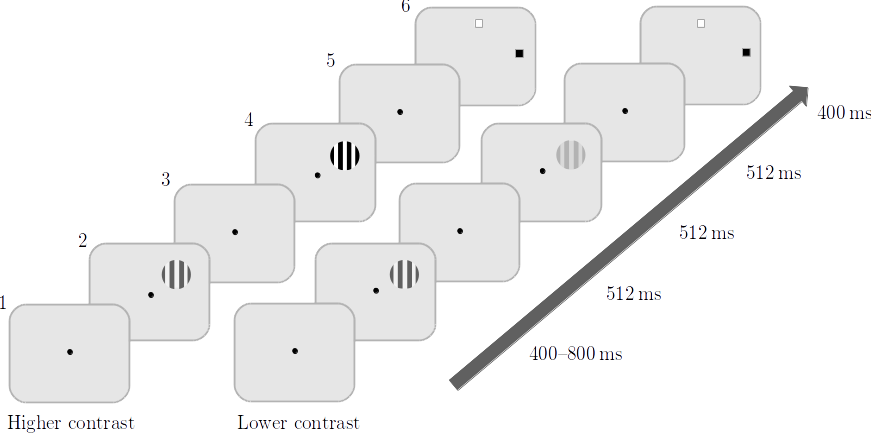
\includegraphics[width=\linewidth]{./figs/info/PLtask1.png}
\end{center}
\caption{
Experimental procedure.
1:~The monkey fixates upon a central spot. 2:~A sample stimulus in the form of either a Gabor patch or a sine grating is presented at the pedestal contrast (\eg{}~30\%). 3:~Blank sample-test interval. 4:~Test stimulus presented. 5:~Blank test-target interval. 6:~Two target stimuli appear to the left and right of the test stimulus location, signalling that the subject is allowed make a saccade to their chosen target.
Subject's overall objective is to make a comparison between the contrasts of the sample and test stimuli (presented during steps 2 and 4, respectively): if the test stimulus was of a higher contrast (\eg{}~32\%) than the pedestal contrast, they should saccade to the white target, otherwise if the second patch was of lower contrast (\eg{}~28\%), they should saccade to the black target (step 6).
Durations shown are approximates as the actual durations vary slightly depending on the animal: see Table.~\ref{tab:tptimes} for more accurate values.}
\label{fig:pltask1}
\end{figure}

After the monkey has been fixated on the fixation point for a randomised period of time
$t_1$,
a grey-scale Gabor function with a contrast $C_{sample}$ appears on the screen. We refer to this as the \textit{sample stimulus}, and it appears in the animal's field of vision such that it is retinotopic to the location of the implanted brain region.
This Gabor stimulus remains on screen for $t_2$, after which it vanishes.
There follows a delay of $t_3$, during which the animal must continue to fixate on the fixation point.
After this, a second Gabor stimulus with contrast $C_{test}$ appears in the same location as the sample stimulus, also for $t_4$. We refer to this as the test stimulus.
There is then a delay of $t_5$ before the fixation target vanishes and a pair of black and white response target squares appear in a region away from the stimulus location. The monkey is tasked with saccading to the white target if the test stimulus has lower contrast than the sample, or the black target if test has higher contrast. If the monkey responds correctly, it is immediately given a water reward. The experiment is thus a two-alternate forced-choice experiment.
After the animal has given its response, the next trial begins without delay, and the fixation target again appears alone on the screen until the monkey has fixated for some randomised duration $t_1$.
The durations used for each part of the experiment are given in Table.~\ref{tab:tptimes}.

\begin{table}[hbtp]
\caption{Durations of each section of the trials.
$t_1$:~interval from fixation-start until sample presentation.
$t_2$:~sample presentation.
$t_3$:~sample-test stimulus interval.
$t_4$:~test presentation.
$t_5$:~test-targets interval.
Differing monitor refresh rates for the two monkeys results in different durations because stimuli can only be presented at the start of the monitor refresh cycle.
\NB{}~A random duration for $t_3$ was used when the experiment was performed on M1 in V4, but this was changed to a static delay for data collected later.}
\label{tab:tptimes}
\begin{center}
\begin{tabular}{rlr}
\toprule
Animal  & Region & Time ($\unit{ms}$)
% \\
%         &       & Inter-trial delay
\\
\midrule
M1  & V4    & $530.872 \le t_1 \le 545.526$
\\
        & V1    & $525.803 \le t_1 \le 538.983$
\\
M2    & V4    & $526.295 \le t_1 \le 540.641$
\\
        & V1    & $525.834 \le t_1 \le 540.702$
% \\
% \midrule
%         &       & Sample presentation duration
\\
\midrule
M1  & V4    & $t_2 = 529.275$ 
\\
        & V1    & $t_2 = 529.275$
\\
M2    & V4    & $t_2 = 533.176$
\\
        & V1    & $t_2 = 533.176$
% \\
% \midrule
%         &       & Post-sample stimulus delay
\\
\midrule
M1  & V4    & $539.720 \le t_3 \le 1058.673$
\\
        & V1    & $t_3 = 541.164$
\\
M2    & V4    & $t_3 = 546.632$
\\
        & V1    & $t_3 = 546.570$
% \\
% \midrule
%         &       & Test presentation duration
\\
\midrule
M1  & V4    & $t_4 = 529.275$
\\
        & V1    & $t_4 = 529.275$
\\
M2    & V4    & $t_4 = 533.176$
\\
        & V1    & $t_4 = 533.176$
% \\
% \midrule
%         &       & Post-test stimulus delay
\\
\midrule
M1  & V4    & $t_5 = 423.475$
\\
        & V1    & $t_5 = 423.475$
\\
M2    & V4    & $t_5 = 426.578$
\\
        & V1    & $t_5 = 426.640$
\\
\bottomrule
% \toprule
%         &       & Time(ms)
% \\
% Animal  & Brain region & $t_1$  & $t_2$  & $t_3$  & $t_4$   & $t_5$
% \\
% \midrule
% M1  & V4    & $530.872 \le t_1 \le 545.526$   & $t_2 = 529.275$  & $539.720 \le t_3 \le 1058.673$  & $t_4 = 529.275$  & $t_5 = 423.475$
% \\
%         & V1    & $525.803 \le t_1 \le 538.983$   & $t_2 = 529.275$  & $t_3 = 541.164$  & $t_4 = 529.275$  & $t_5 = 423.475$
% \\
% M2    & V4    & $526.295 \le t_1 \le 540.641$   & $t_2 = 529.275$  & $t_3 = 546.632$  & $t_4 = 533.176$  & $t_5 = 426.578$
% \\
%         & V1    & $525.834 \le t_1 \le 540.702$   & $t_2 = 533.176$  & $t_3 = 546.570$  & $t_4 = 533.176$  & $t_5 = 426.640$
% \\
% \bottomrule
\end{tabular}
\end{center}
\end{table}

Following a period of rest after surgery, during which the implants should settle into stable locations, the animals are pre-trained to sit in the chair and fixate on the fixation point. They are then trained in the procedure of the experiment, whilst recordings are taken from V4. Their preliminary training involves a grey disc as the sample, whilst the test is either white or black. This then changes to be a set of Gabor functions.
% check this


After the preliminary training, the main perceptual learning experiment is performed, first for V4, then V1.
In the main experiment, we keep the contrast of the sample as $C_{sample} = 30\%$ throughout.

The test contrast is chosen from a set of 14 contrasts:
\{10, 15, 20, 25, 27, 28, 29, 31, 32, 33, 35, 40, 50, 60\}\% for V1 and
 \{5, 10, 15, 20, 22, 25, 28, 32, 35, 40, 45, 50, 60, 90\}\% for V4,
for both of the animals. These groups are chosen such that the animal has a similar initial accuracy for both V1 and V4. We note that half of the contrasts are above and half below the sample contrast of 30\%.
The contrast is not chosen randomly at the start of each trial; instead a batch of trials containing a set number of each test contrast is placed into sequence all at once.
If the monkey responds incorrectly at the end of the trial, this contrast is added to a list to be repeated at the end of the batch.
At the end of the batch, another batch of trials begins in a similar fashion.
% This \textit{delayed repeat} method is used because ...
%(This will be an important fact later in the study.)

The duration of daily training was typically limited by the animal's desire to preform the task. On some days the animal was reluctant to train at all and only 250 trials could be conducted; whilst on other days the animal would be willing to train for three hours and complete up to 1250 trials.
As expected, the psychometric performance of the monkey increased each day for around 20 days due to perceptual learning. After the performance stayed the same for 5 consecutive days, the experiment progressed to the next stage.


\begin{figure}[htbp]
\begin{center}
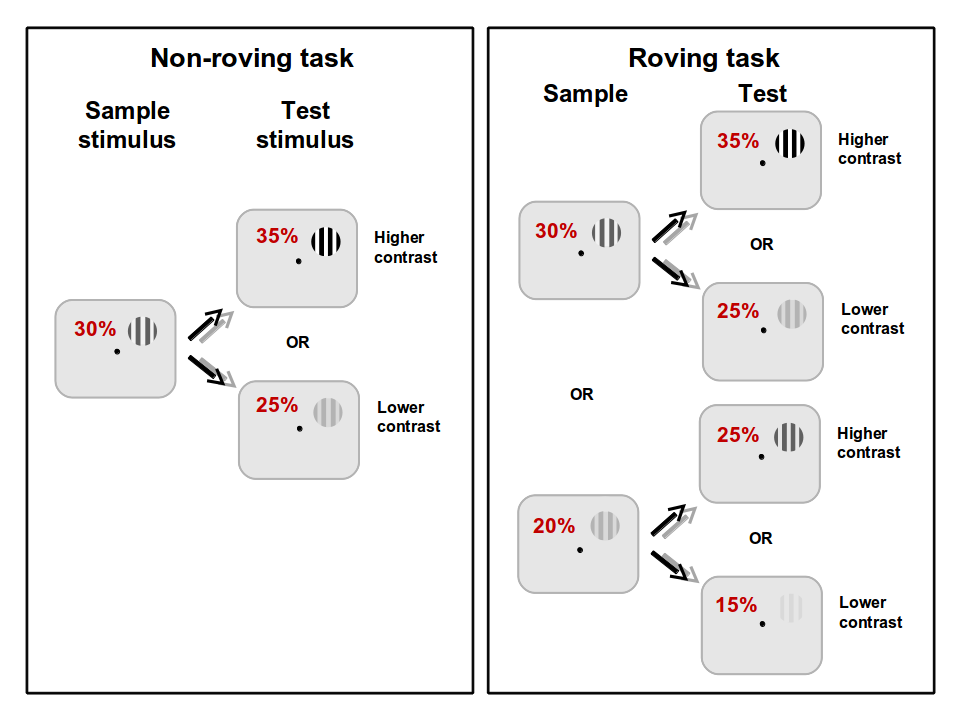
\includegraphics[width=0.8\linewidth]{./figs/info/PLtask2.png}
\end{center}
\caption{The experimental task during both the non-roving and roving stages. The analysis contained in this report concerns only the first, non-roving, stage.}
\label{fig:pltask2}
\end{figure}

% \begin{figure}[htbp]
% \begin{center}
% 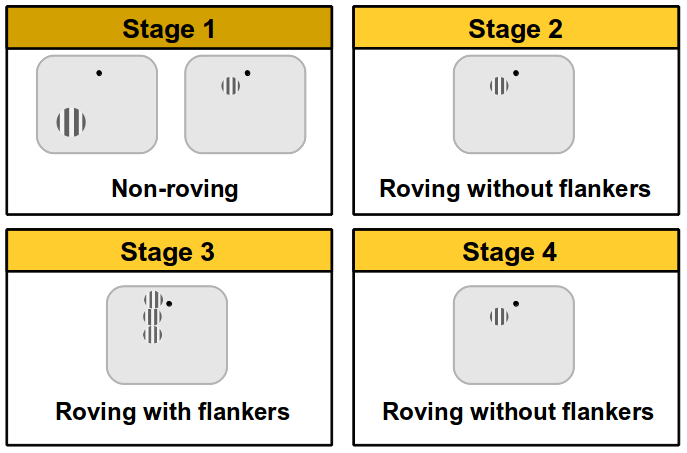
\includegraphics[width=0.8\linewidth]{./figs/info/PLtask3.png}
% \end{center}
% \caption{The experiment was composed of 4 stages. In this analysis, we are concerned only with the first stage.}
% \label{fig:pltask3}
% \end{figure}

In this study, we will focus on analysing data from the non-roving perceptual learning task as described above. However, it should be noted that once the animals had completed the non-roving stage of the experiment, they progressed to further stages involving a roving task. In the roving task, the sample contrast was chosen at random with $C_{sample} \in \{20, 30, 40\}\%$. Subsequently, once the test stimulus had been shown and the targets appeared, the animal was tasked with responding by comparing the test contrast to whichever sample contrast was presented on that particular trial. During this task, the test contrast would be selected from a set of 12 contrasts specific to each of the three sample stimuli, such that 6 test stimuli were higher and 6 lower in contrast than the sample. The difference between the non-roving and roving stages is illustrated in Fig.~\ref{fig:pltask2}.
%
% One small inconsistency in the experimental setup is that for M1 during the V4-based task, the inter-stimuli wait was chosen randomly as $t_3 \in [x,y]ms$. For later experiments, including the V1 recordings for M1 and both V4 and V1 recordings for M2, the inter-stimuli wait was fixed at $t_3 = z ms$.

As mentioned in Sec.~\ref{sec:bgpl}, some previous research has found flankers around the stimuli are necessary to induce perceptual learning.
During this experiment, the researchers found flankers were not necessary for perceptual learning during the first stage, but to subsequently learn to the roving task, flankers around the stimuli were necessary.

% A related experiment to investigate which neural receptors are important for perceptual learning to take place has been undertaken on a third monkey. This monkey, Frank, has been exposed to neuropharmacological agents to see how they affect perceptual learning; the two agents used are the NMDA-receptor antagonist APV, and the muscarinic and nicotinic receptor antagonist scopolamine.

%----------------------------------------------------------------------------------------------------------------------
% \chapter{Data Analysis}
%----------------------------------------------------------------------------------------------------------------------
\section{Spike-Sorting}
\label{sec:sorting}

The initial intention in this study was to first analyse the pre-filtered continuous data using an automated spike detection and sorting program. The output from the automated sorting would then be used for the main portion of the study and analysed using information theoretic techniques.
The motivation for using an automated spike-sorting program was three-fold.

Firstly, data recordings are collected from an array of intracellular electrodes. After thresholding the continuous data to extract the spikes, we will be left with spikes from a handful of neurons closest to the electrode, with different peak voltages depending on their distance from the recording electrode. Since different not all neurons behave in the same manner, we would like to isolate individual neurons for the following analysis.

Secondly, automated spike-sorting will use the same rules to sort the spikes for every session throughout the experiment, so the results will be very consistent. In comparison to this, sorting spikes manually by eye is subjective, and it is impossible even for the same human to apply exactly the same methodology every time they perform the process.

Thirdly, sorting spikes manually is very time consuming, and not practical to do within the time constraints of this project.

%----------------------------------------------------------------------------------------------------------------------
\subsection{Methods}

Before the project began, a candidate spike-detection and spike-sorting program, \textit{Wave Clus}, was identified.%
\footnote{
\textit{Wave Clus} is available online at
\url{http://www2.le.ac.uk/departments/engineering/research/bioengineering/neuroengineering-lab/spike-sorting}
}

The extracellular voltage recordings include the spikes of any neurons surrounding the microelectrode and background noise (from more distant spikes), on top of the more gradual changes in local field potential (LFP). These voltage recordings have already been low- and high-pass filtered to isolate the voltage signals from the LFP and spikes respectively.

In order to best study the information content of the spiking data, we need to know the spike times of individual neurons \cite{Quiroga2009}. Since each neuron will give a characteristic spike profile in the voltage trace, specific to the type neuron, its intracellular properties, and its distance from the microelectrode, it is possible to group together the spikes which come from the same neurons \cite{Quiroga2007}.
This is done by applying spike-detection and spike-sorting algorithms to the high-pass filtered data.

This method involves spike-detection with a threshold of
$$
%\text{thr}
\theta
= \frac{4}{0.6745} \operatorname{median} \left( |x| \right)
,$$
followed by a wavelet transformation of the spikes, and then superparamagnetic clustering on the 10 wavelet coefficients which provide the maximum variance to group the spikes together for specific neurons~\cite{Quiroga2004}.
In a related paper, Rodrigo Quian Quiroga \etal{} found that in tests with simulated data this method outperforms older techniques such as using PCA for feature extraction and $K$-means for clustering~\cite{Quiroga2004}.

%----------------------------------------------------------------------------------------------------------------------
\subsection{Results}
\label{sec:sorting-result}

It was found that, despite the author's claims of offering a fully automated spike-sorting algorithm, in reality the output from \textit{Wave Clus} needed manual adjustment to merge the neurons sorted at different temperatures during the superparamagnetic clustering into a single set of neurons.

For example, the raw data might contain spikes from 3 different neurons. The software performs superparamagnetic clustering at a variety of temperatures, starting too low (paramagnetic phase) so that all the spikes are clustered together, and ending up too high (ferromagnetic phase) so there are about far too many clusters of spikes, say 50. Inbetween, there is a superparamagnetic phase, in which there are a few clusters each of a reasonable size, and this is where it is hoped that the optimal sorting lies.

However, the superparamagnetic phase spans a wide range of temperatures, so when left completely unsupervised, the software chooses the highest temperature at which a cluster containing more than 60 points appears as the optimal temperature. But this neglects the results from other temperatures in the superparamagnetic region, and it is perfectly plausible that there is one temperature, $T_1$, at which the spikes are clustered in two clusters $C_{1}(T_1)$ and $C_{2}(T_2)$
and another temperature, $T_2$, at which the spikes are clustered in two clusters $C_{1}(T_2)$ and $C_{3}(T_2)$.
The optimal sorting is actually to use three clusters $C_1, C_2, C_3$, but the spikes which belong in these three clusters are not all correct at the same temperature. The user must choose temperature $T_1$, lock the spikes $C_{2}(T_2)$ so they stay there, then move to $T_2$ and let the other spikes move around as appropriate.

The process is somewhat tedious, and not terribly clear.
Furthermore, even if it is not necessary to manually intervene with the clusters, the user is required to check this manually.

Another problem is that the temperatures used during the clustering have to be predefined, and different datasets have different optimal temperatures, so there is no guarantee that the range of temperatures used will find a good sorting of the neurons. Granted, this is an understandable limitation, since it is impractical to endlessly search parameter space, and most of the time the range of temperatures used will be suitable, but it seems that it would not be so difficult to find a good range of temperatures on the fly by checking whether the paramagnetic and ferromagnetic bounds have been found.

In the interests of time and the desire to proceed with the main part of the experiment, the decision was taken to abandon the spike-sorting and use the sortings already performed by the researcher, Xing Chen, who had conducted the experiments. This analysis is presented in the following section.

The recordings were collected and processed using the Neurolynx electrophysiology data recording and processing software suite.
Raw recordings were filtered to include only the frequency band \unit[600--4000]{Hz}, and spikes extracted with a sampling frequency of \unit[32556.000]{Hz}.

The researcher found that for some channels multiple individual neurons could be isolated from the spike-sorting, whilst for many only one neuron was sorted. However, for many of the channels where multiple neurons could be sorted, they could not be reliably sorted for every training session. So for consistency in the analysis over multiple sessions, the spikes from these individual neurons were merged together.

%----------------------------------------------------------------------------------------------------------------------
%----------------------------------------------------------------------------------------------------------------------
%----------------------------------------------------------------------------------------------------------------------
\chapter{Information Theoretic Analysis}
%----------------------------------------------------------------------------------------------------------------------

As mentioned in Sec.~\ref{sec:sorting-result}, the automated spike sorting had to be abandoned. The dataset used in this section consists of spiking activity manually sorted by the researcher who collected the data.

%----------------------------------------------------------------------------------------------------------------------
\subsection{Methods}

To best illustrate the process gone through in the study, we include some preliminary results amongst the methods.
This is presented so the reader will better understand the decisions taken whilst progressing with the analysis.

%----------------------------------------------------------------------------------------------------------------------
\FloatBarrier
\subsubsection{Artifact elimination}
\label{sec:ma}

Looking at rasters generated to include all the trials across all the sessions, an anomaly was apparent.
For several of the channels in the data from each of the brain regions of each of the animals, some sessions have spikes which align at the same time relative to the stimulus onset. The temporal alignment is very precise, indicating the effect not part of the animal's brain activity but instead due to an external source influencing the detected signal in the recordings. Furthermore, the ``lines'' occurred at regularly spaced intervals, with a period very nearly equal to the refresh rate of the monitor. The spikes across multiple trials line up like this because the experimental equipment will only begin presenting a stimulus when the first pixel on the monitor is being updated, and we of course normalise for the stimulus presentation time across multiple trials.
% INCLUDE RASTER EXAMPLE

An empirical estimate of the artifact periodicity was found by choosing an arbitrary channel which strongly expresses the artifact and measuring by eye the duration of the completed artifact cycles within \unit[530]{ms} (44 for M1, 39 for M2). Since the artifact is tightly localised in time, this could be done with relatively high accuracy. For M1, the period was estimated to be \unit[85.023(1)]{Hz}, whilst for M2 it was \unit[75.023(1)]{Hz}. The discrepancies from the programmed monitor refresh rates of \unit[85]{Hz} and \unit[75]{Hz} respectively can be put down to the specific electronic circuitry used, perhaps issuing the command to the monitor. The discrepancy is small enough to be of little consequence, except we will need \unit[5]{sf} of accuracy rather than \unit[2]{sf} in the following treatment of the artifact. Why it should be out by exactly \unit[0.023]{Hz} for both animals remains unclear, since this corresponds to the refresh cycle running \unit[0.0031]{ms} fast for M1 and \unit[0.0042]{ms} fast for M2. An even bigger mystery is how the artifact has made its way into the recordings. Although it remains possible that the cause is some other piece of equipment also locked to the same refresh cycle, in the following we will refer to this artifact as the ``monitor artifact''. When a collection of datapoints exhibits the monitor artifact, we refer to the data as ``contaminated''.

From the rasters, it seemed as if three-quarters of the channels in M1 V4 were contaminated for at least one session; over two-thirds of the channels for M1 V1 and M2 V4 were contaminated for at least one session; and around a third of the channels for M2 V4 were contaminated for at least one session. The contaminated channels include both high-quality channels with a lot of detected spikes, and low-quality channels with fewer detected spikes. For some of the lowest quality channels and sessions, the artificial spikes were clearly more numerous than the genuine ones. It was considered paramount that the effects of the artifact be corrected for.

To clean up the contamination, a more rigorous method of evaluating the problem was required.
For the collection of spike times from a single channel across multiple trials during a single session, we perform the following steps:
\begin{enumerate}
\item Consider the set of all spiketimes where the visual stimulus has been the same for at least the last \unit[150]{ms}.
\item From each spiketime, $t$, subtract time of nearest stimulus onset/offset, $T_{\text{onset}}$. (Both onset and offset are synchronised with the monitor cycle, and the nearest one offers greatest accuracy.)
$$
t \leftarrow t - T_{\text{onset}}
$$
\item Take the modulo of the spiketimes with respect to the monitor period, $\tau_m$ (\unit[11.7616]{ms} for M1, \unit[13.3292]{ms} for M2).
$$
t \leftarrow t \bmod \tau_m
$$
\item Take a histogram of the spiketimes over bins with the width of the reciprocal of the sampling frequency of the spikes (sampling frequency \unit[32556.000]{Hz}; bin width \unit[0.030716]{ms}).
\end{enumerate}
Conceptually, this is equivalent to stacking all the ``lines'' in the raster on top of each other and seeing how thick the resulting line is.
When the visual stimulus has remained unchanged for at least \unit[150]{ms}, the neurons in V1 and V4 settle down to a steady firing rate, so we expect there to be about the same number of spikes in each of these bins. However, as the monitor artifact increases the number of spikes at set intervals after the monitor refresh commences, there will be an increase in the number of spikes in these bins when the monitor artifact is manifest in the data.

% ./figs/monitor_hist_blanco_v4_ch4_s336_20120817T085037.eps
% ./figs/monitor_hist_jack_v1_ch9_s51_20120817T084845.eps
% ./figs/monitor_hist_jack_v1_ch9_s56_20120817T084855.eps
% ./figs/monitor_hist_jack_v4_ch41_s31_20120817T085111.eps
%%\begin{figure}[htbp]
%%    \begin{subfigure}[b]{0.5\linewidth}
%%        \centering
%%        \caption{}
%%        \label{fig:mahist-b4}
%%        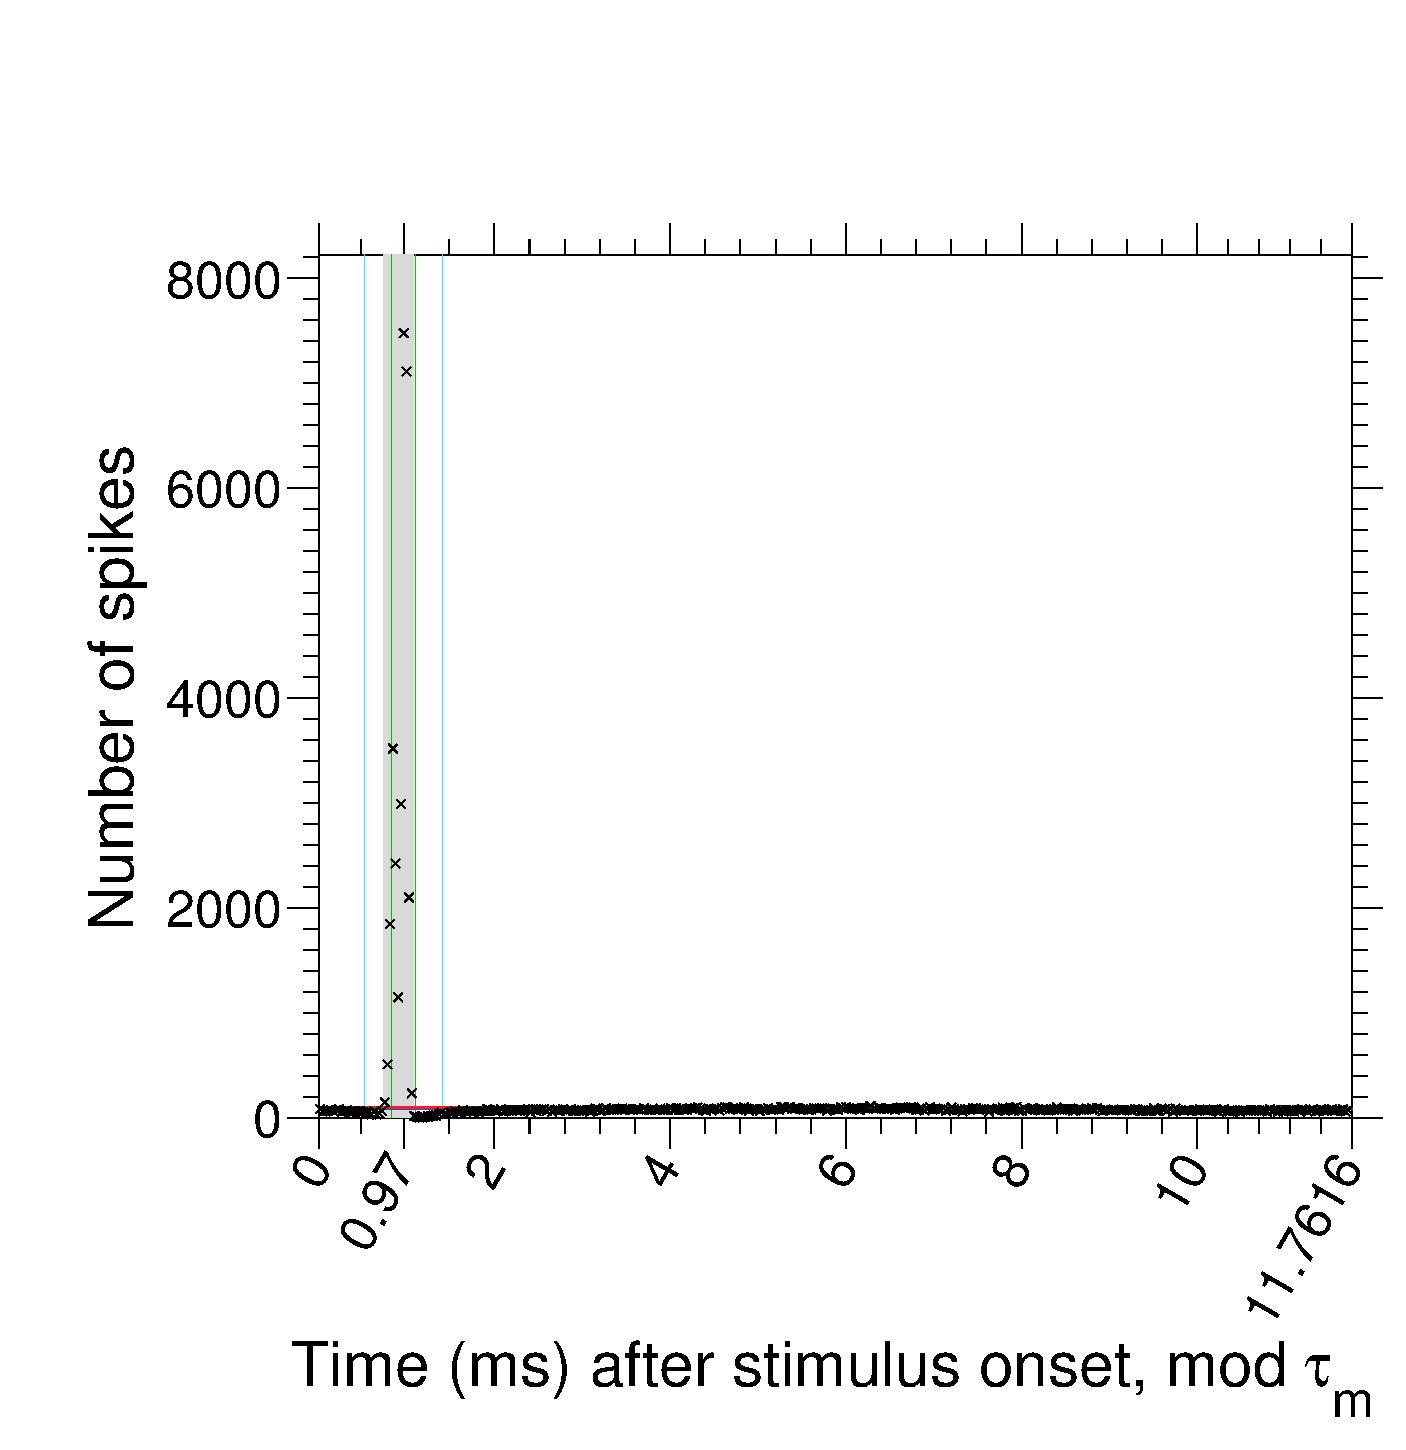
\includegraphics[width=\linewidth]{%
%%./figs/monitor_hist_blanco_v4_ch4_s336_20120817T085037.eps}
%%    \end{subfigure}
%%    ~~
%%    \begin{subfigure}[b]{0.5\linewidth}
%%        \centering
%%        \caption{}
%%        \label{fig:mahist-j4}
%%        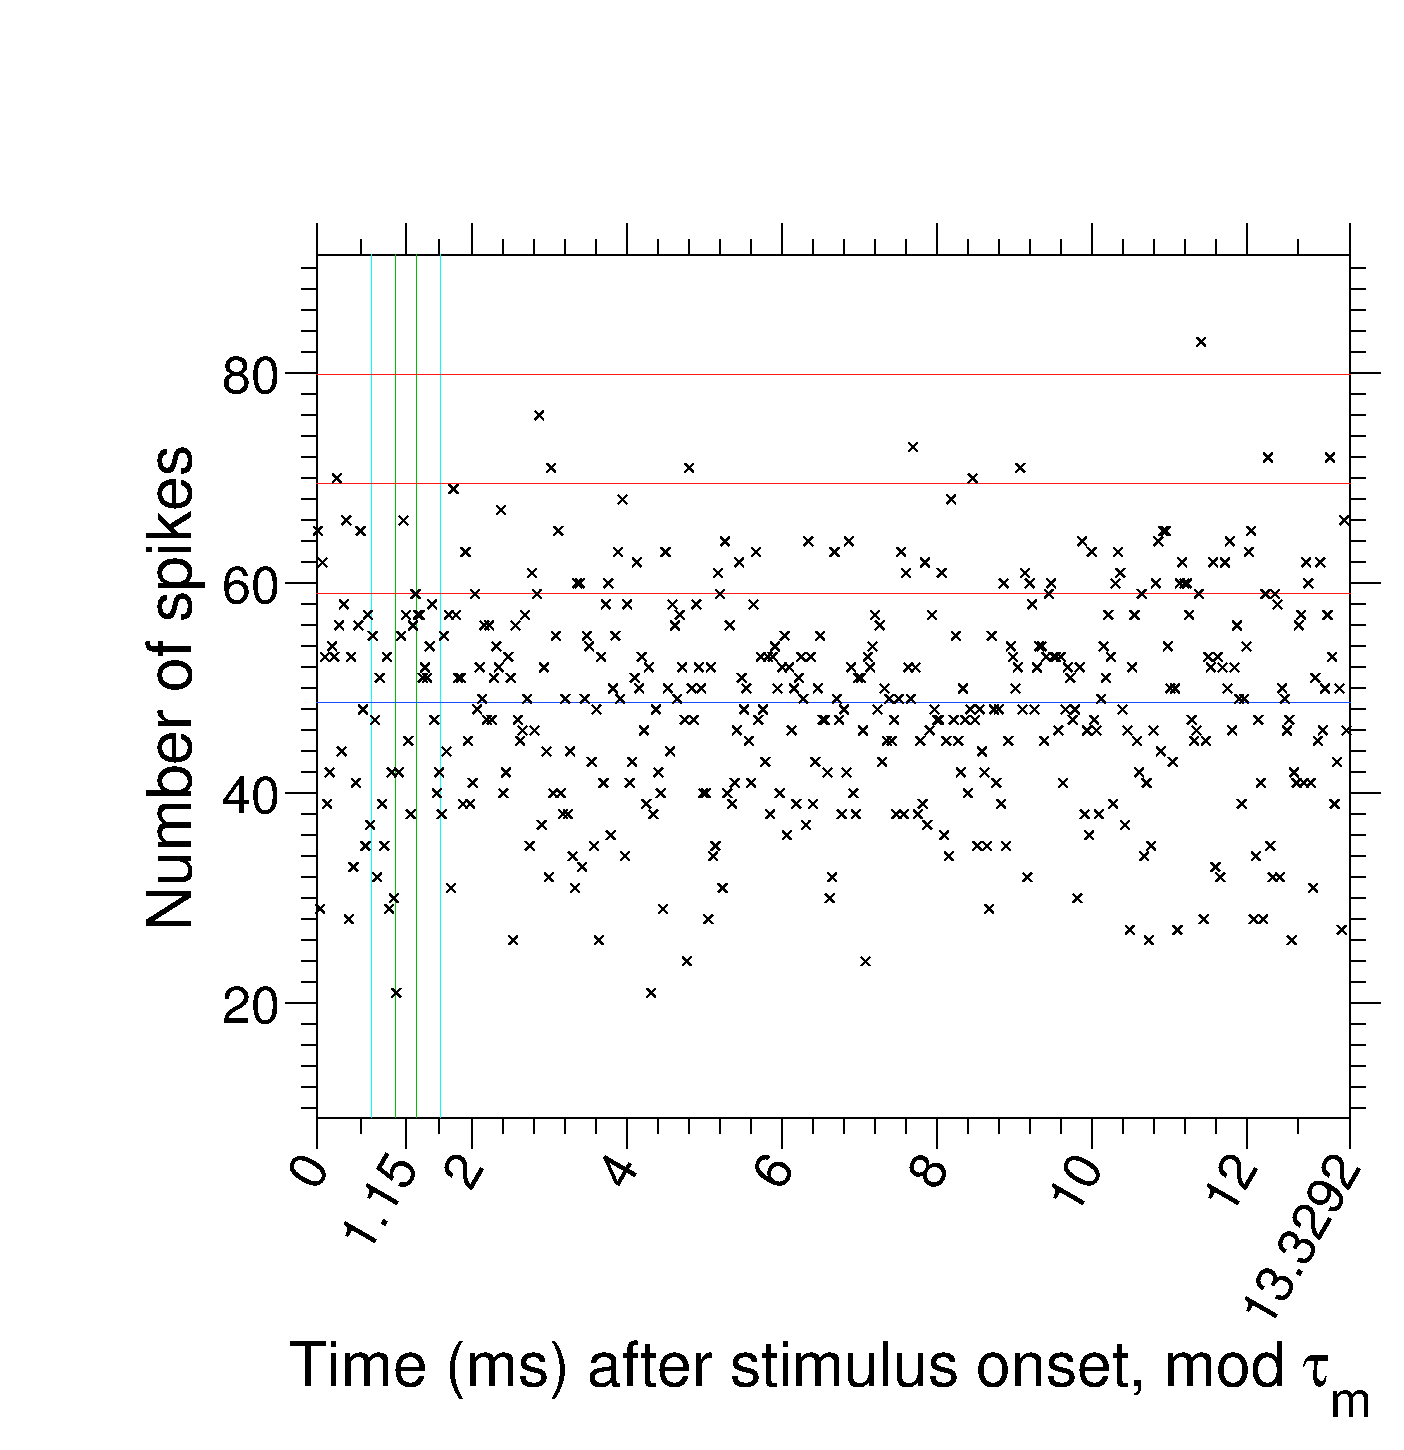
\includegraphics[width=\linewidth]{%
%%./figs/monitor_hist_jack_v4_ch41_s31_20120817T085111.eps}
%%    \end{subfigure}
%%    \\
%%    \begin{subfigure}[b]{0.5\linewidth}
%%        \centering
%%        \caption{}
%%        \label{fig:mahist-j1s51}
%%        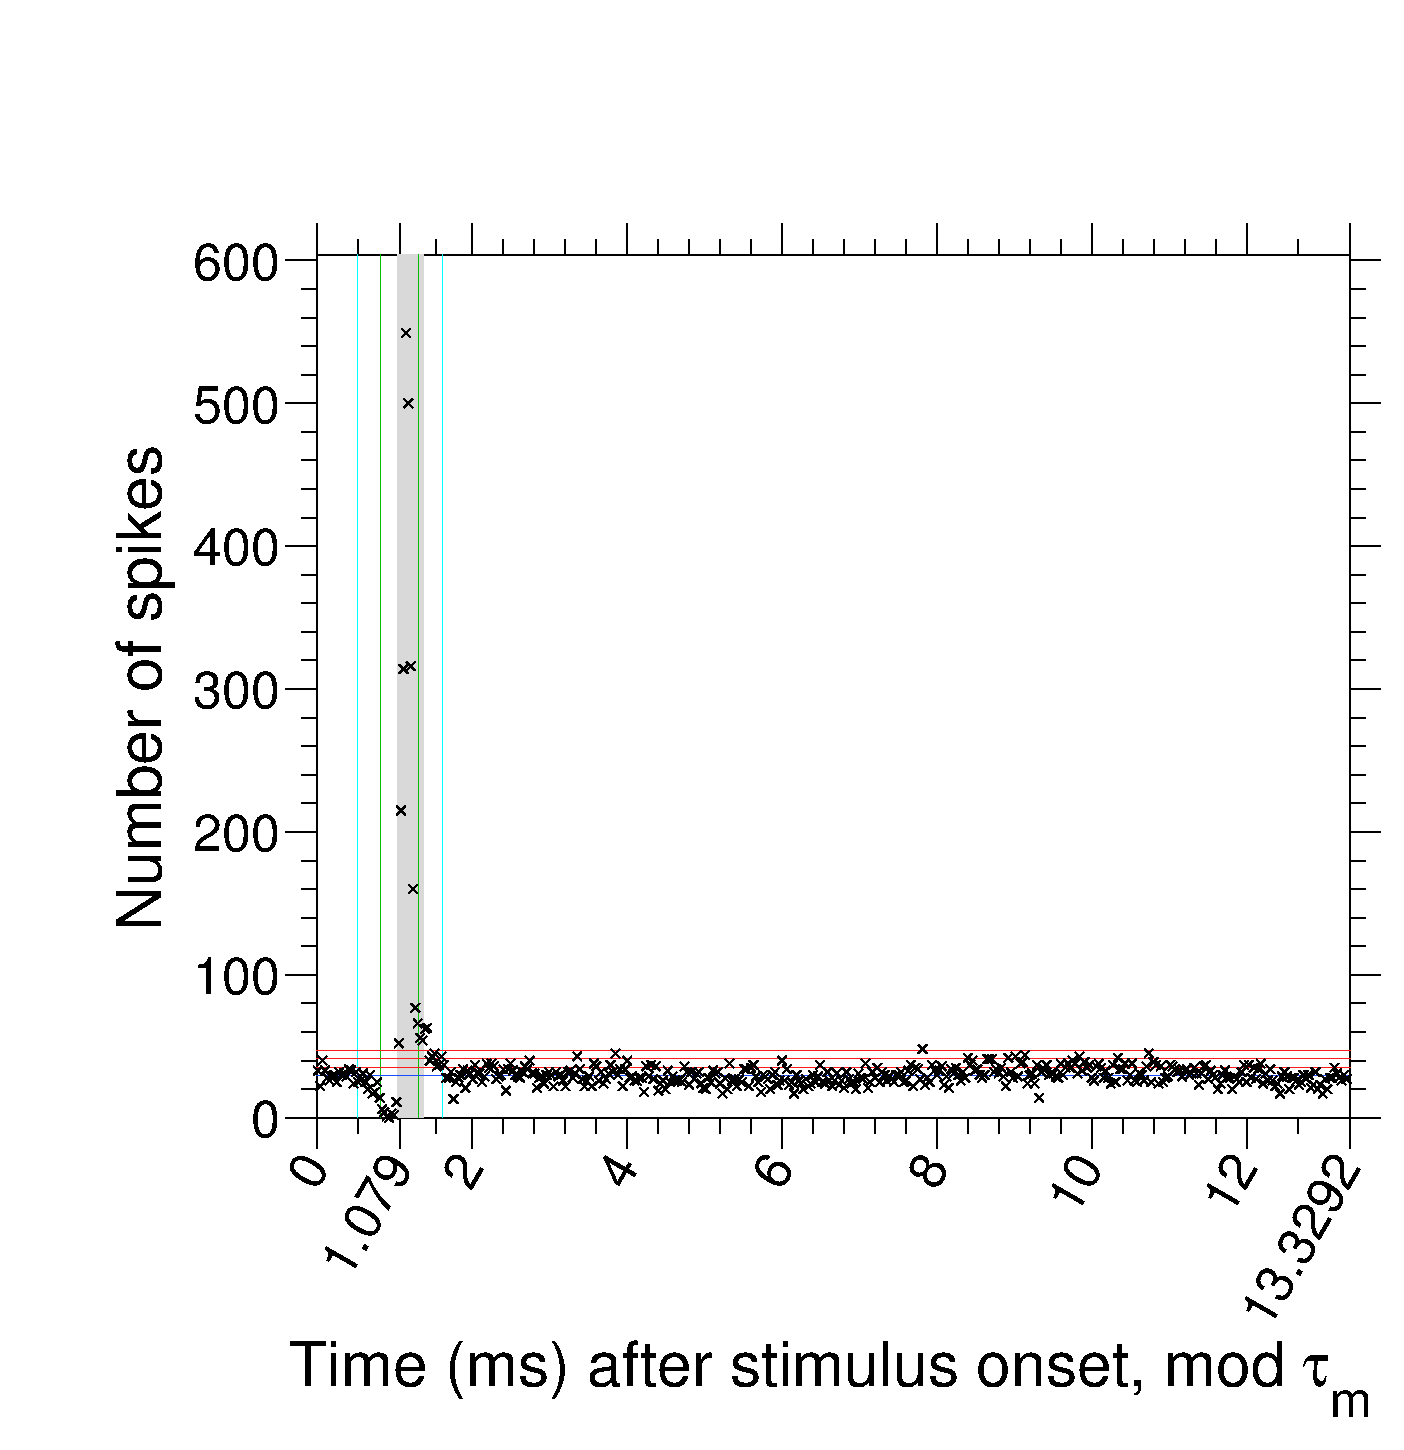
\includegraphics[width=\linewidth]{%
%%./figs/monitor_hist_jack_v1_ch9_s51_20120817T084845.eps}
%%    \end{subfigure}
%%    ~~
%%    \begin{subfigure}[b]{0.5\linewidth}
%%        \centering
%%        \caption{}
%%        \label{fig:mahist-j1s56}
%%        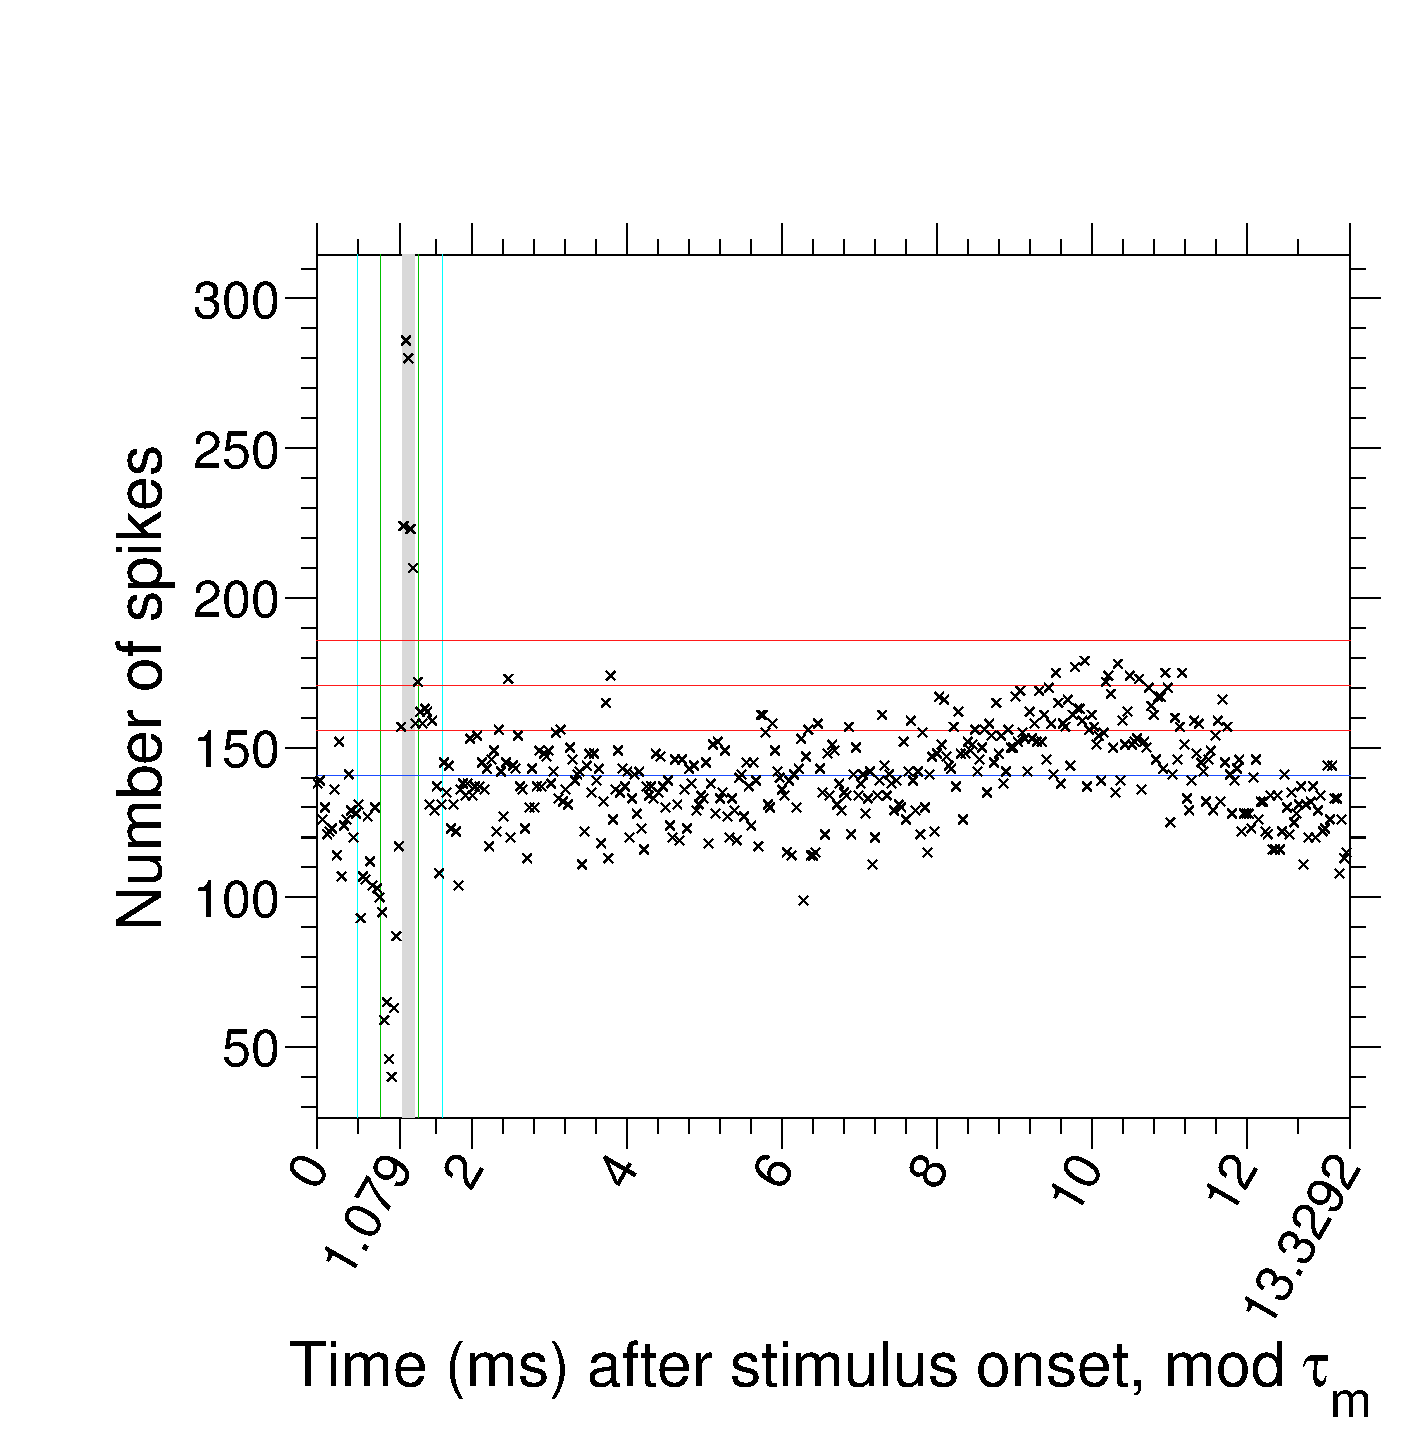
\includegraphics[width=\linewidth]{%
%%./figs/monitor_hist_jack_v1_ch9_s56_20120817T084855.eps}
%%    \end{subfigure}
%%    \caption{Crosses: Histogram of spikes in bins of width \unit[0.030716]{ms}.
%%\ref{fig:mahist-b4}: M1 V4, channel 4, session 336; a channel and session very strongly exhibiting the monitor artifact.
%%\ref{fig:mahist-j4}: M2 V4, channel 41, session 31; a dataset where the artifact is not present.
%%\ref{fig:mahist-j1s51}: M2 V1, channel 9, session 51; data strongly presenting the monitor artifact.
%%\ref{fig:mahist-j1s56}: M2 V1, channel 9, session 56; data mildly showing the effect of the monitor artifact.
%%Green vertical lines: extremities of search window (contained between the lines).
%%Cyan vertical lines: extremities of mean region.
%%Blue line: mean of the data (excluding area between cyan lines).
%%Red lines: mean plus 1, 2 and 3 standard deviations respectively.
%%Gray background: Spikes marked as contaminated and scheduled for redaction.
%%}
%%    \label{fig:mahist}
%%\end{figure}

% INSERT HIST FIGURE 

As shown in Fig.~\ref{fig:mahist}, the analysis conforms to our expectations.
However, doing the analysis in this more rigorous manner revealed the contamination was more widespread than previously assumed. The histograms of spiketimes indicate that more sessions are contaminated than not, and only a couple of channels are completely clean for every session.

For the most part, the timing of the monitor artifact $\bmod \tau_m$ is very reliable and it affects the same 6 or so bins whenever the data is contaminated. The contaminated part of each monitor cycle is thus restricted to at most \unit[0.2]{ms}, and, assuming this period of time contains both genuine spikes and artificial spikes, if we simply delete all datapoints with this \unit[0.2]{ms} window, we will lose at most less than 2\% of the genuine spikes. This level of data loss is not terribly significant, and justifiable for the gain in reliability of the remaining dataset, particularly for sessions where artificial spikes seem to be more common than genuine ones.

\begin{table}[hbtp]
\caption{Typical time of the peak in number of spikes due to the monitor artifact effect. The time is given relative to the start of the monitor refresh as given by the stimulus onset times. Monitor artifacts occur at $t = t^*_m + k \tau_m$, for $k \in \Z$. For channels recording from M2 V1, the artifact will occur at one of the two stated times throughout a given session, but which of the two varies from channel-to-channel for any individual session, and from session-to-session for any individual channel. Why this happens is unclear.}
\label{tab:mapeak}
\begin{center}
\begin{tabular}{rlc}
\toprule
Animal  & Region & Time of artifact peak $t^*_m$ $\pm 0.01$ (\unit{ms})
\\
\midrule
M1  & V1    & 0.95
\\
        & V4    & 0.97
\\
M2    & V1    & either 0.97 or 1.19
\\
        & V4    & 1.15
\\
\bottomrule
\end{tabular}
\end{center}
\end{table}

% However it is apparent that this method is not great (see jack v1 ch7 s57)

However, it is possible to do better that this and to isolate and remove only the contaminated bins. As shown in Fig.~\ref{fig:mahist}, the effect of the artifact is greater for some sessions than others and
From observations on the typical width time of the width and peak time (Table.~\ref{tab:mapeak}) of the artifact, along with its periodicity ($\tau_m$), the following method of removal was devised and implemented.
\begin{enumerate}
\item Perform the modulo $\tau_m$ and take the histogram as described above.
\item Define the ``search region'' as bins which contain spike within $t^*_m \pm \unit[0.130]{ms}$, so we have one bin more than the anticipated artifact width in either direction. (For M2 V1, we use the range \unit[$(0.968 - 0.130 , 1.190 + 0.130)$]{ms}.)
\item Find the mean, $\mu$, and standard deviation, $\sigma$, of all the bins which are at least 10 away (\unit[0.3]{ms} away) from the search region. We also exclude the final bin since $0.030716 \bmod \tau_m \neq 0$ and it is only part-full.
\item If any one of the bins in the search region exceeds $\mu + 3 \sigma$, we declare the session contaminated and proceed with the following steps. If not, it is declared intact and left as it is.
\item All bins in the search region which contain more than $\mu + 3 \sigma$ spikes are declared contaminated.
\item Let $t_m$ denote the time of the centre of the bin in the search region containing the most spikes.
\item All bins which contain spikes within $t_m \pm \unit[0.1]{ms}$ are placed in ``quarantine''.
\item All quarantined bins which contain more than $\mu + 2.5 \sigma$ spikes are declared contaminated.
\item All bins between the first and last contaminated bins are declared contaminated.
\item Consider immediate neighbours of the first bin and if they are also contain more than $\mu + 2.5 \sigma$ spikes, they are declared contaminated.
\item Repeat the above step until either a neighbour is found which is not contaminated, or until a maximum of three bins have been added to the contaminated region.
\item Consider immediate neighbours of the last bin and if they are also contain more than $\mu + 2.5 \sigma$ spikes, they are declared contaminated.
\item Repeat the above step until either a neighbour is found which is not contaminated, or until a maximum of three bins have been added to the contaminated region.
\item Consider the full dataset of spikes for this particular channel and session.
\item For each spike, consider which bin its spiketime would be arranged into.
\item If it is a contaminated bin, the spike is removed from the dataset.
\end{enumerate}

This allows us to have prior assumptions about the location and width of the monitor artifact effect, but be flexible about exactly where it falls and which sets of bins are affected.
It is possible that the dynamically targeted removal method may cause issues due to inconsistency in the data across different sessions, but there is a clearly a gain in the amount of preserved data and a gain in the reliability of the data which remains.

%----------------------------------------------------------------------------------------------------------------------
\FloatBarrier
\subsubsection{Session-based analysis}

merged all neurons together for a single channels

Neurolynx NSE files were loaded into MATLAB using the Neurolynx supplied code when operating on Windows, and an version 6 of an unofficial port for Linux (recommended by Neurolynx) otherwise.%
\footnote{Available at
\\ \url{http://www.urut.ch/new/serendipity/index.php?/pages/downloads.html}}

The information was computed for each day of training (hereafter referred to as a session), for each of the channels from which recordings were available. To gauge the typical behaviour of a neuron, the mean was taken over all the channels.
The mutual information between the spiking activity during test presentation and the identity of the test stimulus was computed
using a spike-timing based code.
This computation was done using the \verb|information| function from the freely available Information Break-down Toolbox \cite{Magri2009} for MATLAB.%
\footnote{Available at \url{http://www.ibtb.org}}

A moving window of $\unit[20]{ms}$ was taken and subdivided into 5 sequential bins, each of $\unit[4]{ms}$.
The number of spikes within each of the 5 bins was totalled up to provide a code letter for the bin.
The combination of the 5 sequential counts forms a codeword.

This is performed across all the trials in a session with the $\unit[20]{ms}$ window placed with the same offset relative to the test stimulus onset.
By assembling the trials according to their test contrast, the mutual information between the contrast and the spiking activity in this window can be computed.

Following the methods employed by the research group, only trials in which the monkey responded correctly were used for this analysis.

%----------------------------------------------------------------------------------------------------------------------
% 5bins of 4ms
% ./figs/I_sessionwise_blanco_v1_chmean23_s343-359_oc1_5bins_of_4ms_dr_naive_pcolorhot_20120815T150057.png
% ./figs/I_sessionwise_blanco_v4_chmean31_s307,308,311,313,314,317,318,320,321,329-341_oc1_5bins_of_4ms_dr_naive_pcolorhot_20120815T150100.png
% ./figs/I_sessionwise_jack_v1_chmean25_s51-72_oc1_5bins_of_4ms_dr_naive_pcolorhot_20120815T150049.png
% ./figs/I_sessionwise_jack_v4_chmean20_s24-49_oc1_5bins_of_4ms_dr_naive_pcolorhot_20120815T150053.png
% 1 bin of 20ms
% ./figs/I_sessionwise_blanco_v1_chmean23_s343-359_oc1_1bins_of_20ms_dr_naive_pcolorhot_20120815T190833.png
% ./figs/I_sessionwise_blanco_v4_chmean31_s307,308,311,313,314,317,318,320,321,329-341_oc1_1bins_of_20ms_dr_naive_pcolorhot_20120815T190836.png
% ./figs/I_sessionwise_jack_v1_chmean25_s51-72_oc1_1bins_of_20ms_dr_naive_pcolorhot_20120815T190825.png
% ./figs/I_sessionwise_jack_v4_chmean20_s24-49_oc1_1bins_of_20ms_dr_naive_pcolorhot_20120815T190829.png
% 
% ./figs/I_sessionwise_blanco_v1_chmean23_s343-359_oc1_5bins_of_4ms_dr_naive_pcolorhot_20120815T202102.png
% ./figs/I_sessionwise_blanco_v4_chmean31_s307,308,311,313,314,317,318,320,321,329-341_oc1_5bins_of_4ms_dr_naive_pcolorhot_20120815T202106.png
% ./figs/I_sessionwise_jack_v1_chmean25_s51-72_oc1_5bins_of_4ms_dr_naive_pcolorhot_20120815T202053.png
% ./figs/I_sessionwise_jack_v4_chmean20_s24-49_oc1_5bins_of_4ms_dr_naive_pcolorhot_20120815T202058.png


%%\begin{figure}
%%\centering
%%\subfloat[A big tikz picture.\label{fig:one}]{%
%%  \makebox[\textwidth][l]{% %%% as above
%%  \resizebox{.45\largefigure}{!}{%
%%    \input{fig/tikzfile}}}}%
%%\hfill%
%%\subfloat[Another big tikz picture.\label{fig:two}]{%
%%  \makebox[\textwidth][l]{% %%% as above
%%  \resizebox{.45\largefigure}{!}{%
%%    \input{fig/tikzfile}}}}%
%%\caption{Two tikz pictures}
%%\label{fig:label}
%%\end{figure}
%%
%%\begin{figure}%
%%\centering
%%\subfloat[][]{...figure code...}%
%%\qquad
%%\subfloat[][]{...figure code...}%
%%\caption{Here are the first two figures of a continued figure.}%
%%\label{fig:cont}%
%%\end{figure}

\begin{figure}[htbp]%
    \centering
    \subfloat[][M1 V1.\label{fig:sessb1}]{%
        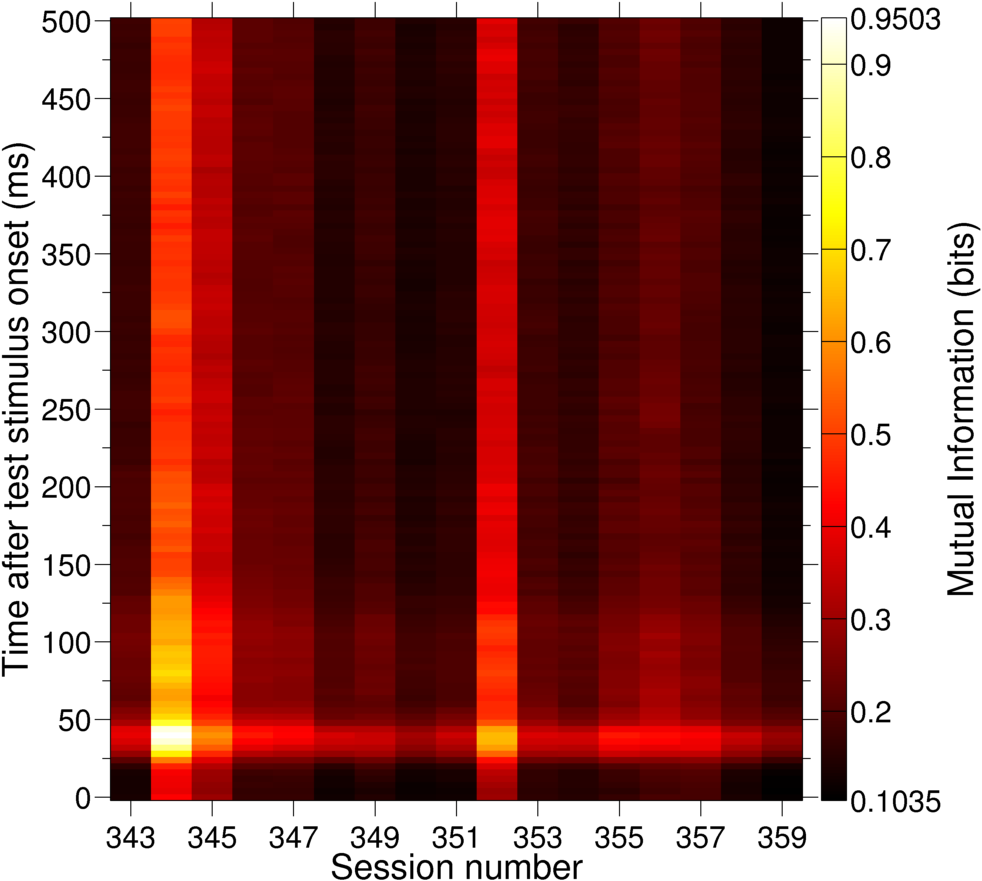
\includegraphics[scale=.25]{%
./figs/I_sessionwise_blanco_v1_chmean23_s343-359_oc1_5bins_of_4ms_dr_naive_pcolorhot_20120815T202102.png}
    }%
    ~~
    \subfloat[][M1 V4.\label{fig:sessb4}]{%
        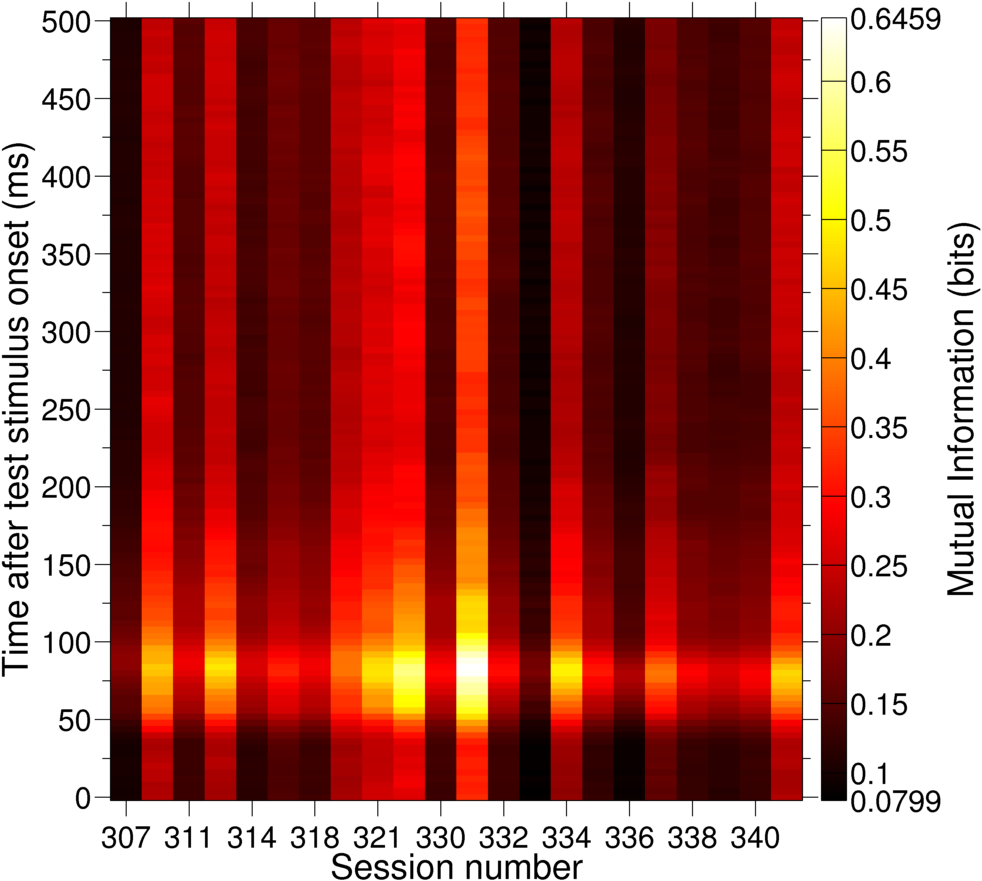
\includegraphics[scale=.25]{%
./figs/I_sessionwise_blanco_v4_chmean31_s307,308,311,313,314,317,318,320,321,329-341_oc1_5bins_of_4ms_dr_naive_pcolorhot_20120815T202106.png}
    }%
    \\
    \subfloat[][M2 V1.\label{fig:sessj1}]{%
        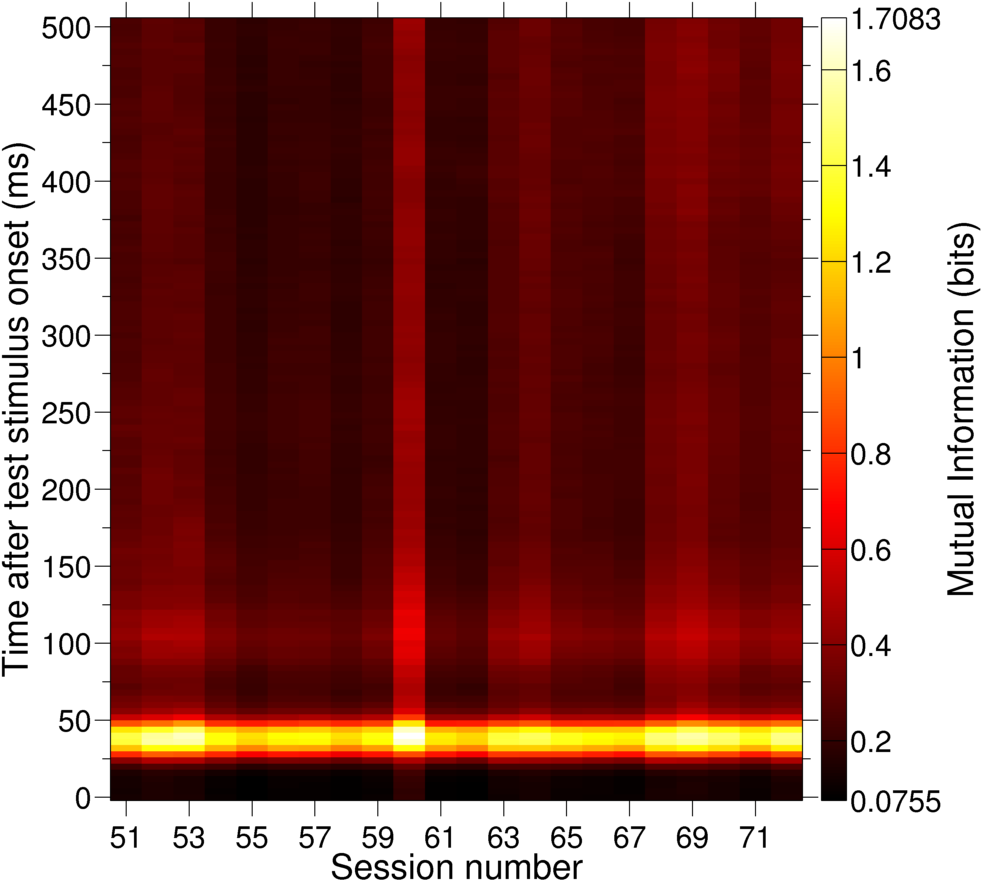
\includegraphics[scale=.25]{%
./figs/I_sessionwise_jack_v1_chmean25_s51-72_oc1_5bins_of_4ms_dr_naive_pcolorhot_20120815T202053.png}
    }%
    ~~
    \subfloat[][M2 V4.\label{fig:sessj4}]{%
        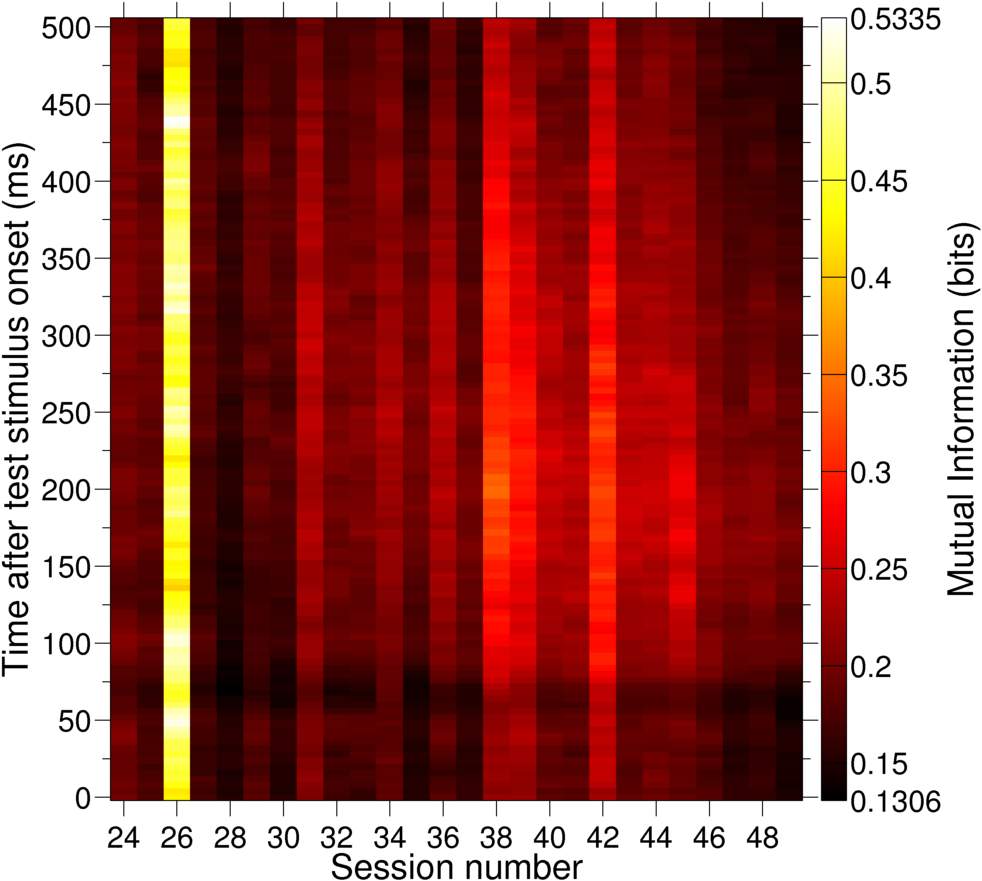
\includegraphics[scale=.25]{%
./figs/I_sessionwise_jack_v4_chmean20_s24-49_oc1_5bins_of_4ms_dr_naive_pcolorhot_20120815T202058.png}
    }%
    \caption{Mutual information between the test stimulus and the neural activity during test presentation.
The mutual information with the test stimulus is taken for a spike timing based code for a \unit[20]{ms} window of spiking activity, sampled with the start of the window offset ($y$-axis) from \unit[0]{ms} up to \unit[500]{ms} after test stimulus onset (which is slightly more than \unit[20]{ms} before test stimulus offset). The sampling is in intervals of \unit[5]{ms}, so any 4 adjacent squares within each session are highly correlated.
The recording session number for the data is given along the $x$-axis, and the number of days the animal has been trained for increases from left to right.
Average mutual information across all the channels is denoted by the pseudo-colour of each of the rectangular patches, centred around the $(x,y)$ co-ordinate to which the measurement relates.
In each case the average is taken across all available channel data: \ref{fig:sessb1}~23 channels, \ref{fig:sessb4}~30 channels, \ref{fig:sessj1}~25 channels, \ref{fig:sessj4}~20 channels.
% The PT bias correction method was used (see text).
The plug-in method without bias correction was used (see text).
}
    \label{fig:sess}
\end{figure}

% ./figs/I_sessionwise_blanco_v1_chmean23_s343-359_oc1_5bins_of_4ms_dr_pt_pcolorhot_20120811T130028.eps
% ./figs/I_sessionwise_blanco_v4_chmean31_s307,308,311,313,314,317,318,320,321,329-341_oc1_5bins_of_4ms_dr_pt_pcolorhot_20120811T130522.eps
% ./figs/I_sessionwise_jack_v1_chmean25_s51-72_oc1_5bins_of_4ms_dr_pt_pcolorhot_20120811T130003.eps
% ./figs/I_sessionwise_jack_v4_chmean20_s24-49_oc1_5bins_of_4ms_dr_pt_pcolorhot_20120811T133212.eps

The results of this initial analysis are shown in Fig.~\ref{fig:sess}.
% Although the relationship between different window offsets and the mutual information is similar for each of the sessions, the
No trend in information content with learning can be discerned because the measured mutual information content varies wildly from session-to-session.

% %----------------------------------------------------------------------------------------------------------------------
% \chapter{}
% %----------------------------------------------------------------------------------------------------------------------
% \subsection{Methods}


% Demonstrate how this is dominated by the number of trials in the session, regardless of bias correction technique

% ./figs/ntrialsIbyNindiv_blanco_v1_dr_naive_20120812T164553.eps
% ./figs/ntrialsIbyNindiv_blanco_v4_dr_naive_20120812T164553.eps
% ./figs/ntrialsIbyNindiv_jack_v1_dr_naive_20120812T164553.eps
% ./figs/ntrialsIbyNindiv_jack_v4_dr_naive_20120812T164553.eps
%
% ./figs/ntrialsIandNindiv_blanco_v1_dr_naive_20120812T175154.eps
% ./figs/ntrialsIandNindiv_blanco_v4_dr_naive_20120812T175154.eps
% ./figs/ntrialsIandNindiv_jack_v1_dr_naive_20120812T175154.eps
% ./figs/ntrialsIandNindiv_jack_v4_dr_naive_20120812T175154.eps
%
% ./figs/ntrialsIandNindiv_blanco_v1_dr_naive_1bins_of_20ms_20120815T200333.eps
% ./figs/ntrialsIandNindiv_blanco_v4_dr_naive_1bins_of_20ms_20120815T200333.eps
% ./figs/ntrialsIandNindiv_jack_v1_dr_naive_1bins_of_20ms_20120815T200333.eps
% ./figs/ntrialsIandNindiv_jack_v4_dr_naive_1bins_of_20ms_20120815T200333.eps
% 
% ./figs/ntrialsIandNindiv_blanco_v1_dr_naive_5bins_of_4ms_20120815T201856.eps
% ./figs/ntrialsIandNindiv_blanco_v4_dr_naive_5bins_of_4ms_20120815T201856.eps
% ./figs/ntrialsIandNindiv_jack_v1_dr_naive_5bins_of_4ms_20120815T201856.eps
% ./figs/ntrialsIandNindiv_jack_v4_dr_naive_5bins_of_4ms_20120815T201856.eps
% 
% % \begin{figure}[htbp]
% %     \begin{subfigure}[b]{0.5\linewidth}
% %         \centering
% %         \caption{M1 V1}
% %         \label{fig:IandNb1}
% %         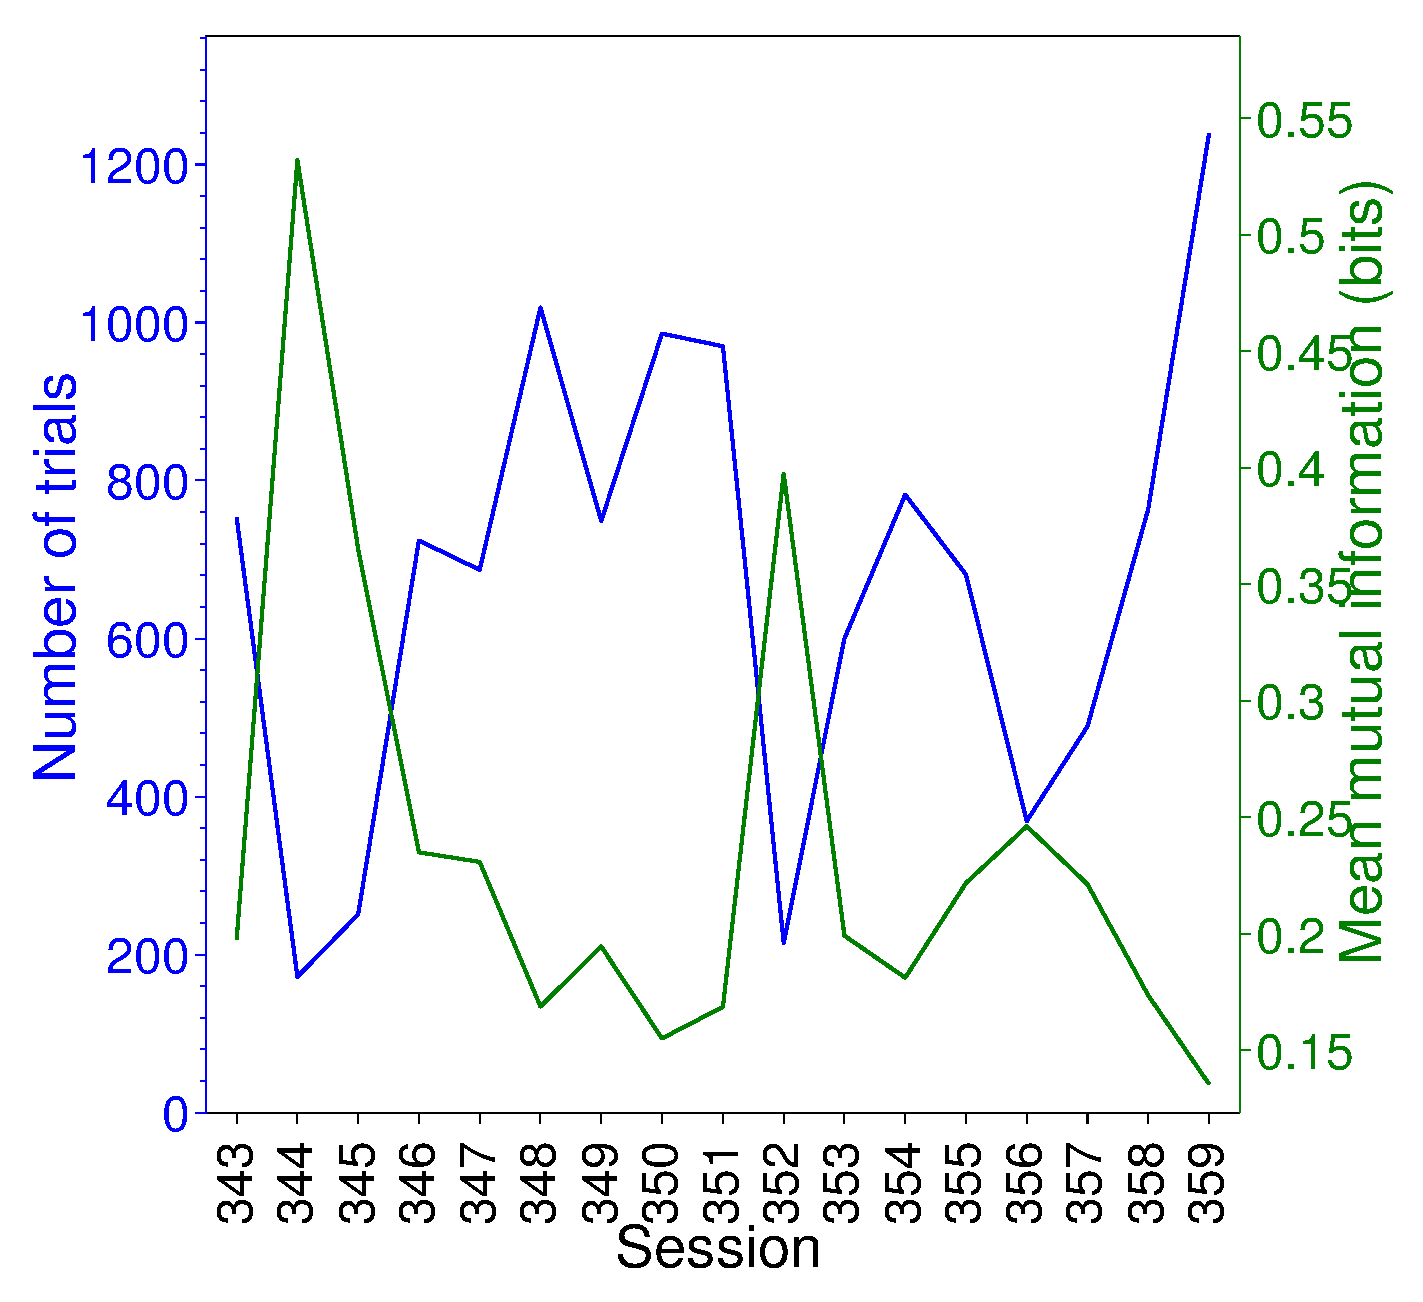
\includegraphics[width=\linewidth]{%
% % ./figs/ntrialsIandNindiv_blanco_v1_dr_naive_5bins_of_4ms_20120815T201856.eps}
% %     \end{subfigure}
% %     \begin{subfigure}[b]{0.5\linewidth}
% %         \centering
% %         \caption{M1 V4}
% %         \label{fig:IandNb4}
% %         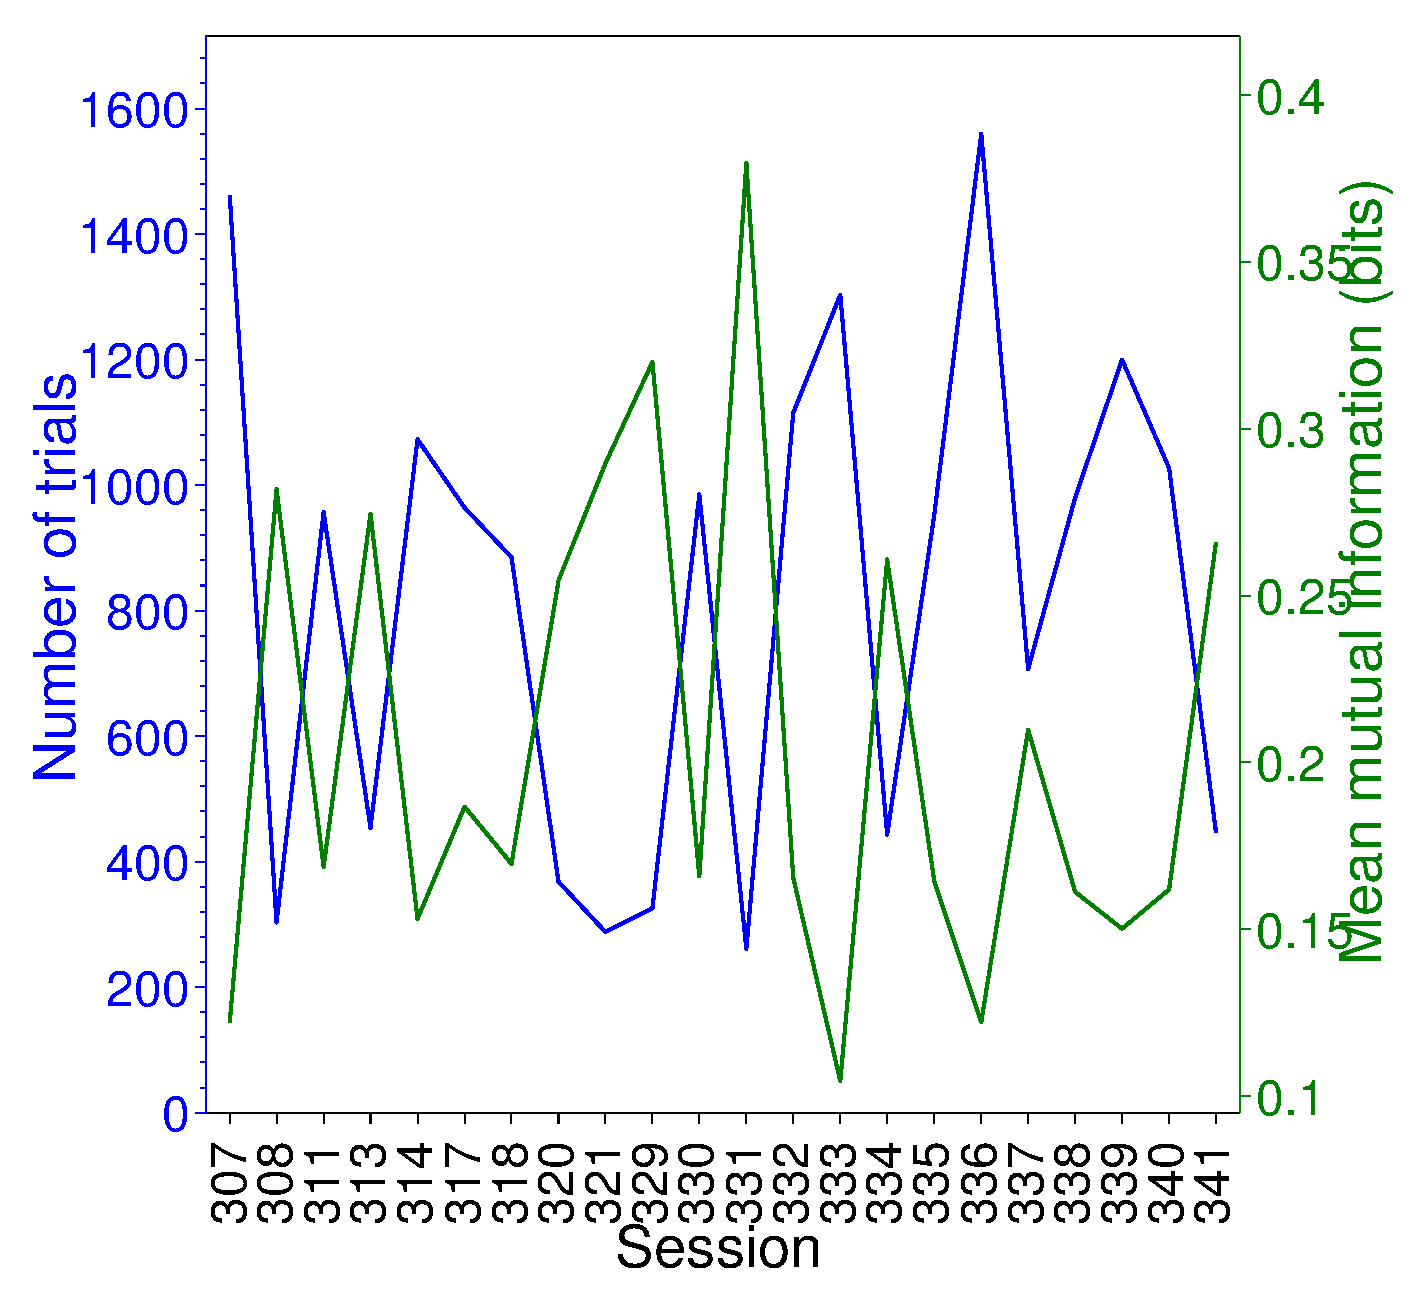
\includegraphics[width=\linewidth]{%
% % ./figs/ntrialsIandNindiv_blanco_v4_dr_naive_5bins_of_4ms_20120815T201856.eps}
% %     \end{subfigure}
% %     \\
% %     \begin{subfigure}[b]{0.5\linewidth}
% %         \centering
% %         \caption{M2 V1}
% %         \label{fig:IandNj1}
% %         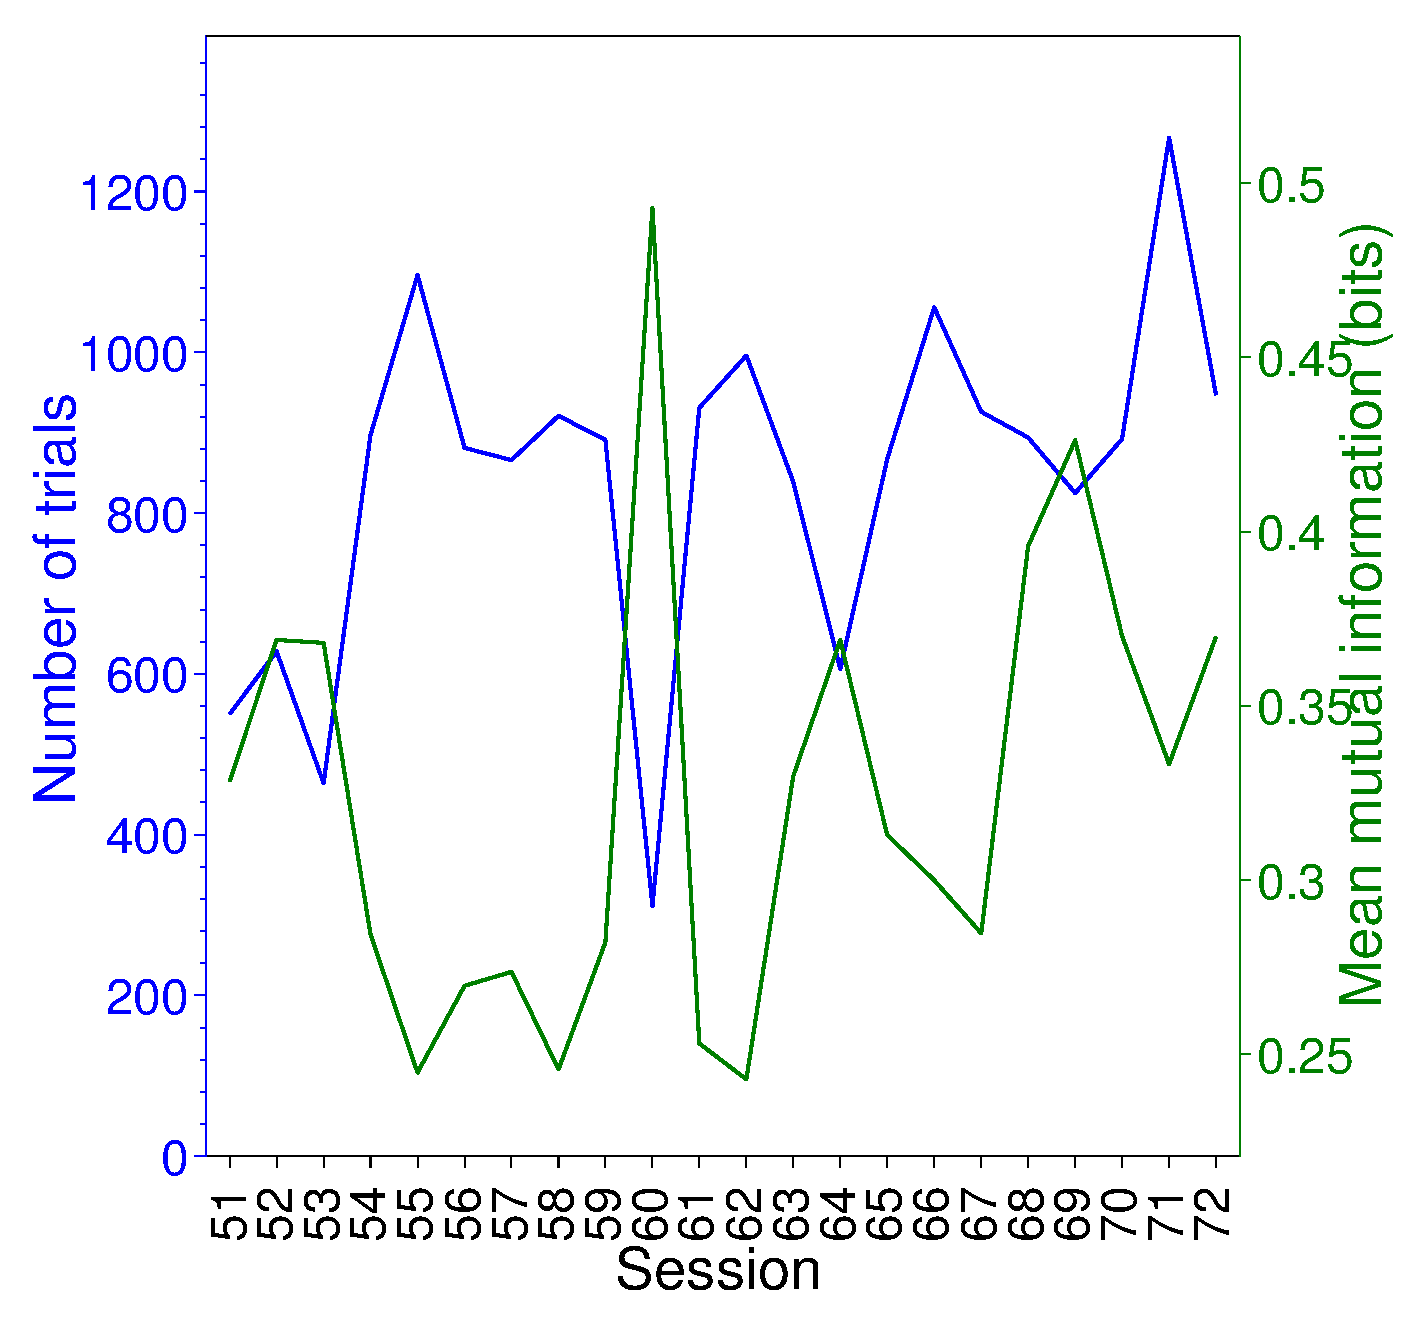
\includegraphics[width=\linewidth]{%
% % ./figs/ntrialsIandNindiv_jack_v1_dr_naive_5bins_of_4ms_20120815T201856.eps}
% %     \end{subfigure}
% %     \begin{subfigure}[b]{0.5\linewidth}
% %         \centering
% %         \caption{M2 V4}
% %         \label{fig:IandNj4}
% %         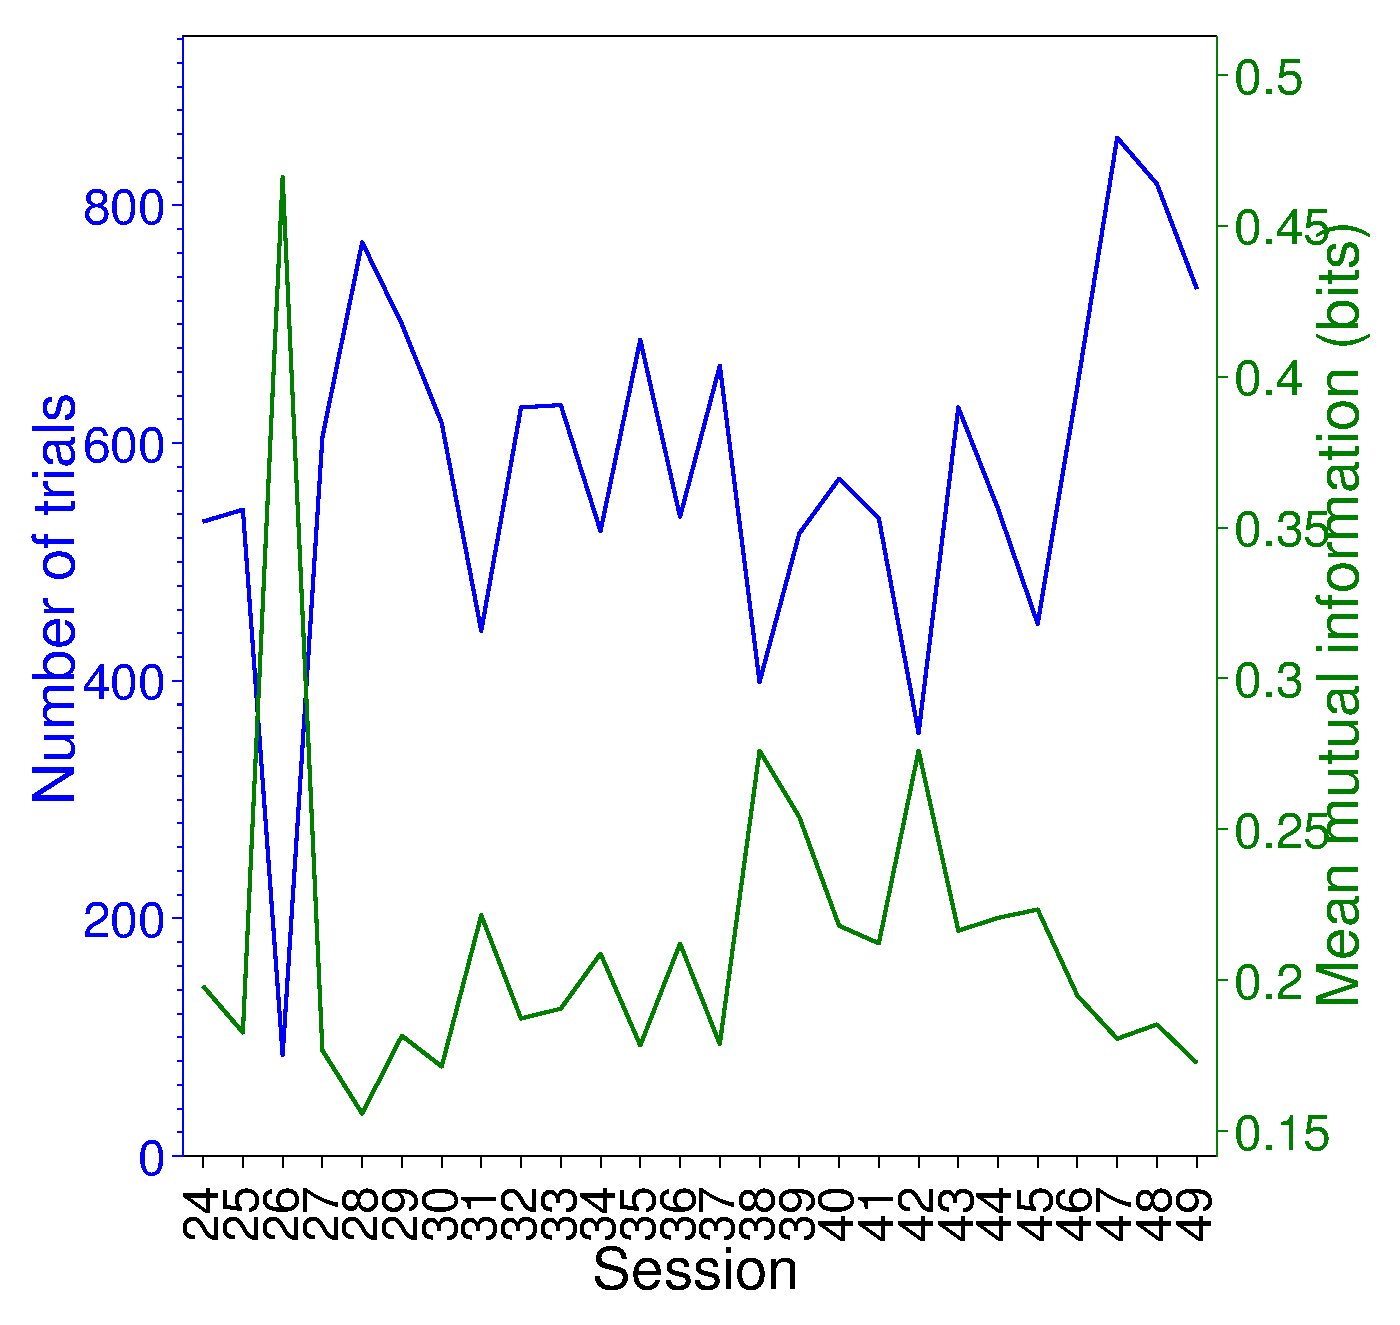
\includegraphics[width=\linewidth]{%
% % ./figs/ntrialsIandNindiv_jack_v4_dr_naive_5bins_of_4ms_20120815T201856.eps}
% %     \end{subfigure}
% %     \caption{Mutual information seems to be anti-correlated with the number of trials in the session. The number of correctly responded trials in each session is plotted on top of the mean information in individual sessions. The mutual information is the ``plug-in estimate'', not corrected for bias, and averaged across the whole period of test stimulus presentation.
% % %There is a missing data point for M2 V4 because in one session there were not enough trials per condition for the QE algorithm to function.
% % }
% %     \label{fig:IandN}
% % \end{figure}

Fig.~\ref{fig:IandN} shows that the changes in the measured mutual information are dominated by the number of trials in the session, not by increases with perceptual learning (corresponding to increments in the session number).
The only exception to this rule seems to be for M2 V1, shown in Fig.~\ref{fig:IandNj1}, where the information increases with learning despite an increase in the number of trials per session over this period.

% ./figs/ntrialsIvsinvNcombindiv_blanco_v1_20120812T164553.eps
% ./figs/ntrialsIvsinvNcombindiv_blanco_v4_20120812T164553.eps
% ./figs/ntrialsIvsinvNcombindiv_jack_v1_20120812T164553.eps
% ./figs/ntrialsIvsinvNcombindiv_jack_v4_20120812T164553.eps
% 
% ./figs/ntrialsIvsinvNcombindiv_blanco_v1_5bins_of_4ms_20120815T204808.eps
% ./figs/ntrialsIvsinvNcombindiv_blanco_v4_5bins_of_4ms_20120815T204808.eps
% ./figs/ntrialsIvsinvNcombindiv_jack_v1_5bins_of_4ms_20120815T204808.eps
% ./figs/ntrialsIvsinvNcombindiv_jack_v4_5bins_of_4ms_20120815T204808.eps
% 
% % \begin{figure}[htbp]
% %     \begin{subfigure}[b]{0.5\linewidth}
% %         \centering
% %         \caption{M1 V1}
% %         \label{fig:IvNb1}
% %         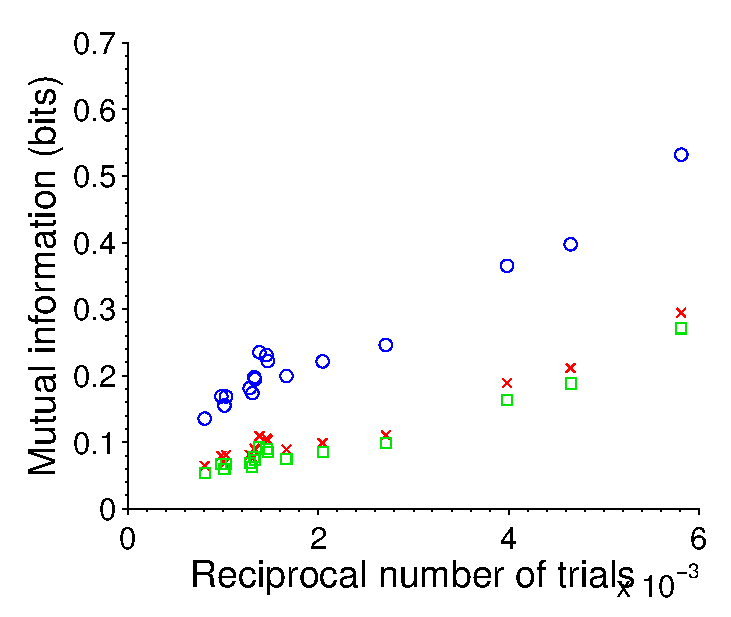
\includegraphics[width=\linewidth]{%
% % ./figs/ntrialsIvsinvNcombindiv_blanco_v1_5bins_of_4ms_20120815T204808.eps}
% %     \end{subfigure}
% %     \begin{subfigure}[b]{0.5\linewidth}
% %         \centering
% %         \caption{M1 V4}
% %         \label{fig:IvNb4}
% %         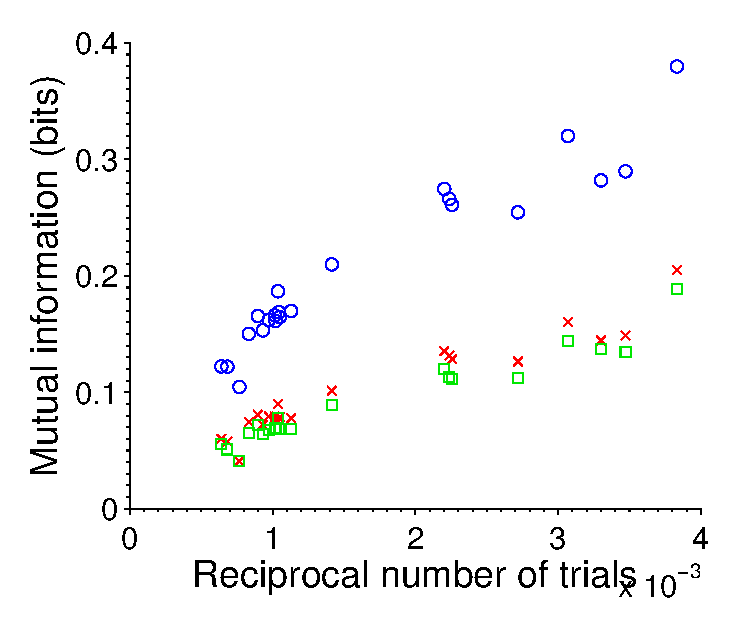
\includegraphics[width=\linewidth]{%
% % ./figs/ntrialsIvsinvNcombindiv_blanco_v4_5bins_of_4ms_20120815T204808.eps}
% %     \end{subfigure}
% %     \\
% %     \begin{subfigure}[b]{0.5\linewidth}
% %         \centering
% %         \caption{M2 V1}
% %         \label{fig:IvNj1}
% %         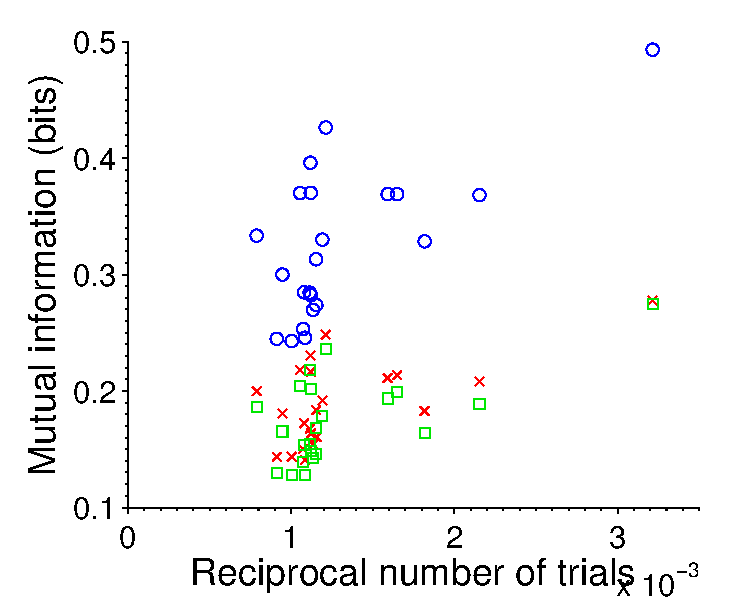
\includegraphics[width=\linewidth]{%
% % ./figs/ntrialsIvsinvNcombindiv_jack_v1_5bins_of_4ms_20120815T204808.eps}
% %     \end{subfigure}
% %     \begin{subfigure}[b]{0.5\linewidth}
% %         \centering
% %         \caption{M2 V4}
% %         \label{fig:IvNj4}
% %         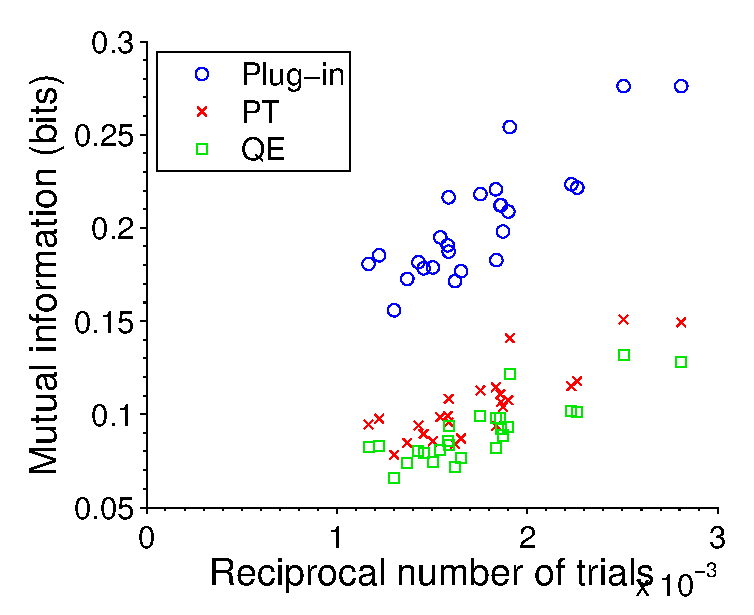
\includegraphics[width=\linewidth]{%
% % ./figs/ntrialsIvsinvNcombindiv_jack_v4_5bins_of_4ms_20120815T204808.eps}
% %     \end{subfigure}
% %     \caption{Mutual information is inversely correlated with the number of trials in the session. The mutual information for a single session is averaged over all channels, and averaged over all times during stimulus presentation, and plotted against the reciprocal of the number of trials in the session ($\nicefrac{1}{N}$). Plug-in:~with no bias correction. PT:~using the Panzeri-Treves method to correct for bias \cite{Panzeri1996}. QE:~using quadratic extrapolation for bias correction \cite{Strong1998}.
% % %There is a missing data point for M2 V4 because in one session there were not enough trials per condition for the QE algorithm to function.
% % }
% %     \label{fig:IvN}
% % \end{figure}

In particular, the measured value for the mutual information is strongly correlated with the reciprocal of the number of trials in the session (Fig.~\ref{fig:IvN}). The correlation is still very strong even if we use one of the two bias correction techniques. As discussed above, for M2 V1 the number of trials per session and the measured information  are both correlated with time, which reduces the correlation observed in Fig.~\ref{fig:IvNj1}.

The problem is that although PT and QE both do a reasonable attempt at removing the bias, they are not perfect and some bias will remain. As the bias is dependent on the number of trials, it is unsurprising the remaining bias follows the same dependency.
In particular, in the asymptotic regime the leading term in the expansion of $I_{\text{measured}}$ is known to be proportional \cite{Treves1995} to $\nicefrac{1}{N}$; the same relationship observed here.

In particular, the difficult faced is changes due to perceptual learning which are of interest may only be slight, but the the number of trials per session varies five-fold: from 250 up to 1250. Consequently it is unsurprising that the observed differences in information day-to-day are dominated by the number of trials.

% %----------------------------------------------------------------------------------------------------------------------
% \subsection{Results}
% 
% %----------------------------------------------------------------------------------------------------------------------
% \chapter{Information Theoretic Analysis (trial-wise)}
% %----------------------------------------------------------------------------------------------------------------------

%----------------------------------------------------------------------------------------------------------------------
\FloatBarrier
\subsubsection{Trial-based analysis}

To counter the correlation between measured information and number of trials, an obvious solution is to use the same number of trials for every computation. We now consider how many trials should be taken at once to obtain a reasonably reliable estimate.

Some rules-of-thumb for the number of trials are offered by \cite{Panzeri2007}.
Let $\overline{R}$ denote the number of possible response codes.
Then, for the plug-in estimate of mutual information, we need to have at least $N_S \ge 2^{32} \, \overline{R}$ trials per stimulus,
whilst if the PT or QE bias correction methods are applied, we only need $N_S > 2 \, \overline{R}$.

% The spike detection software was set to only detect spikes at least \unit[3]{ms} apart, and moreover, 
The probability of having two spikes within \unit[4]{ms} from a non-bursting neuron is very low. For example, a neuron with a high firing rate might fire at \unit[100]{Hz}, which means inter-spike intervals are typically around \unit[10]{ms} (and \unit[100]{Hz} is a high firing rate for the channels in our dataset).
Consequently any \unit[4]{ms} bin will realistically contain either 0 or 1 spikes, and the number of possible response codes in our spike timing code analysis with 5 bins each of \unit[4]{ms} is $\overline{R} = 2^5 = 32$. In comparison for a spike count code, if we assume spikes cannot be closer together than \unit[3]{ms}, there are between 0 and 7 spikes in any \unit[20]{ms} interval. Consequently there are $\overline{R} = 8$ possible response codes.

As we wish our analysis to work for both spike timing and spike count codes, using the above rules we need to use at least 64 trials per stimulus to get a reasonable estimate of the information with one of the bias correction methods in place.
Since there are 14 different stimuli, this means at least 896 trials in total are needed. This presents a dilemma, since most of the sessions are shorter than this, even when both correctly and incorrectly responded trials are included. Excluding sessions with fewer than 896 trials would severely limit the size of the dataset.
% and the patchwork of holes which would result would limit how much can be read into the results due to  which would result.

The solution found was to concatenate the sessions together and analyse groups of $N$ trials taken from multiple consecutive sessions.
The na\"{i}ve justification for this approach is a ``first-order approximation'' to perceptual learning would be that the monkey gets better at recognising the stimuli every-time they perceive it, and so the most important quantifier for the amount of perceptual learning which has taken place is the total number of trials the monkey has performed to date.

This rather basic assumption neglects several factors which influence the animal's performance, such as their mood during the particular training day; and factors which influence the animal's willingness to work (in turn influencing performance), which depends on their recent level of access to water (the reward used in the study). For instance, the animal performs less well on Mondays, which follows on from readily available water during the weekend.
Furthermore, the consolidation which occurs during sleep is commonly believed to be important to perceptual learning, and (as this only occurs between training sessions) this effect is completely ignored by this approach.

However, the session-concatenation approach was attempted regardless, and a value of $N_S = 100$ trials per stimulus was chosen. Though there are enough trials available to use more and reduce the bias further, it is undesirable data from so many sessions at once.

As mentioned in Chap.~\ref{ch:exp}, a delayed repeat is used for any trials to which the animal does not correctly respond. Consequently, more difficult test stimuli (with contrasts close to the sample contrast) are presented significantly more frequently than easier stimuli.
For instance, when presented with the most difficult test stimuli, the animal will have a success rate only just above 50\% on the first day of the experiment, rising to around 70\% by the last day. For the easiest stimuli, the success rate will be nearly 100\% throughout.

Say we arrange all the trials into groups based on their stimulus, then take 100 subsequent trials from each of the groups to perform the analysis on. Due to the different number of trials per stimulus, it will not be long before the trials selected for each stimulus are from very different points in time and from different sessions.\footnote{Even if we only analyse the correctly responded trials, there is still a difference in the number of trials per stimulus due to a limit on the number of repeats of any test condition. The difference was negligible for M1, but accumulated to a 100 trial difference over all the sessions between the most and least correctly responded conditions for M2.}
To ensure all the trials are from when the animal has had the same amount of training, we can instead take a group of $S \cdot N_S = 14 \cdot 100 = 1400$ consecutive trials regardless of the stimulus presented and analysed. The differences in number of trials per stimulus are not particularly important, so long as there are always  enough.

All trials where the monkey completed the trial and gave a response (either correct or incorrect) were included in the analysis. Trials where the monkey did not complete the task by fixating and then providing a response as required were excluded.
Using both the correct and incorrectly responded trials means our distribution for $P(s)$ is the same as that presented to the monkey, and there are notably more trials available to perform the analysis on.

% Using 50 and 100 trials explored: not considerable difference between results. 100 shown for conciseness

%----------------------------------------------------------------------------------------------------------------------
\FloatBarrier
\subsubsection{Information in fine vs. coarse distinctions}

The difference between information about fine differences in contrast can be studied by only considering trials where the contrast presented is one of the middle 6 contrasts:
\{22, 25, 28, 32, 35, 40\}\% for V1 and
\{27, 28, 29, 31, 32, 33\}\% for V4.
To keep the dimensionality of the stimulus the same, this has been compared to the information across some more separated contrasts:
 \{5, 15, 22, 40, 50, 90\}\% for V1 and
\{10, 15, 20, 40, 50, 60\}\% for V4.
For V4, the group of coarsely differentiated contrasts is the outer most six contrasts, but for V1 the coarsely differentiated contrasts are alternate

%----------------------------------------------------------------------------------------------------------------------
\FloatBarrier
\subsubsection{Information in spike timing code vs. spike count code}

Because the possible responses in the spike timing and count codes have different dimensionality, they have different biases \cite{Panzeri2007} and it is not possible to compare them directly.
Consequently, to investigate how much more information there is in a spike timing based code we must consider a set of responses which have the same dimensionality, but lack the timing information.

To do this, the spike-timing response codes are taken, then shuffled across the 5 bins for every individual trial.%
\footnote{The shuffling of bins was performed using the open source Shuffle.m
available from \url{http://www.mathworks.com/matlabcentral/fileexchange/27076-shuffle}.}
Since the 5 bins are now in a random order, any information contained in their order is lost. To make ensure the estimate of the information in the spike-timing code with the timing information destroyed was reasonable, the information was measured for five different shuffles%
% \footnote{The five shuffles were performed with a random seed linked to microsecond of execution time.}
 and then the mean was taken.

The information contained in the \unit[4]{ms} level spike timing can then be found by subtracting the mean shuffled information from the unshuffled information.

%----------------------------------------------------------------------------------------------------------------------
\FloatBarrier
\subsubsection{Spontaneous activity}

To check whether changes in the data quality between sessions and other differences between sessions could be influencing the results, the information theoretic analysis was also applied the spontaneous activity from the animal.
In particular, the spontaneous activity from prior to the sample presentation was used, so the animal had not yet seen the test contrast.
Although monkey's brain activity cannot possibly contain any genuine information about the test contrast, we expect to measure a non-zero value for the information content due to the sampling bias.

%----------------------------------------------------------------------------------------------------------------------
%----------------------------------------------------------------------------------------------------------------------
%----------------------------------------------------------------------------------------------------------------------
\subsection{Results}

During the course of the analysis, results were inspected using PT and using QE for bias correction. The plots were similar in distribution, and each gave a similar magnitude for the information. However, PT gave visibly lower variance than QE, so only plots using PT are presented in this results section.
Using the $I_{\text{sh}}$ approach where the bias is corrected by shuffling bins across trials \cite{Montemurro2007} was also attempted for the spike timing code, but this increased the variance far too much to be of any practical use. The unexpectedly significant increase in variance is probably due to the nature of the correlations between the bins which are being shuffled.

We also compared some of the results both with the monitor artifact left in the data and with the dataset redacted to have it removed. There was no appreciable difference for any of the plots, though the amount of information went down when the data was redacted due to the loss of some of the spikes.

%----------------------------------------------------------------------------------------------------------------------
% \FloatBarrier
% \subsubsection{General Information plots}

Starting with V1, the first thing which is noticed in Figs.~\ref{fig:b1-trialwise} and \ref{fig:j1-trialwise} \ref{fig:b1-1x20tp4} and \ref{fig:b1-5x4tp4} is the large peak in information over the \unit[20]{ms} window starting at around \unit[40]{ms} after stimulus onset. This is due to the onset transient response, where there is a larger amount of neural activity, and this is also less variable than usual \cite{Muller2001}. A second, smaller peak from the ``rebound'' of the transient also occurs around \unit[100]{ms} after stimulus onset. Looking at the scalebars, we can see there is about 10 times as much information on average from the neurons in M2 than M1. This is probably due to differences in data quality between the two animals.

Comparing the information found using the spike timing code \ref{fig:b1-5x4tp4} with the spike count code \ref{fig:b1-1x20tp4}, it seems that there is significantly more information when the binned spike times are considered: there is three times as much information for the spike timing code for M1 and twice as much for M2. However, if we look at information in the spontaneous activity, this reveals we cannot trust this result, as the bias for the information from the spontaneous activity is much higher for the spike timing code than spike count.

For M1, aside from the transient, the information measured with the spike timing code from the spontaneous activity is about the same as the information from the test presentation, suggesting something has gone very wrong!

For the spike timing codes, there is a clear decrease in information with learning in M1, and a clear increase in information for M2. This is, however, present in both the test presentation activity and the spontaneous activity, suggesting it is not a genuine effect. This is believed to be due to a decrease in signal quality in the implants in M1, and possibly an increase in M2.
The increase is also seen in the spike count code for M2, but not to any real extent and it is doubtful that the result is significant.

The bias in the information for the spontaneous activity changes with time for the spike timing code, but does not for the spike count code.
Since any changes in the dataset are the same for both of these, this suggests there are too few trials for the spike timing code to give a reliable reading of the information. This would make sense because with an average of $N_S = 100$ trials per stimulus and a spike timing code with $\overline{R} = 32$, there are
on average $\nicefrac{N_S}{\overline{R}} = 3.125$ trials per response per stimulus,
whilst for a spike count code with $\overline{R} = 8$ there are on average $\nicefrac{N_S}{\overline{R}} = 12.5$ trials per response per stimulus.
Similarly if there we assume a minimum of $N_S = 64$ trials per stimulus, there are
at least $\nicefrac{N_S}{\overline{R}} > 2$ trials per response per stimulus for the spike timing code, and
at least $\nicefrac{N_S}{\overline{R}} > 8$ trials per response per stimulus for the spike count code.

The information in the spontaneous activity was subsequently computed with an average of $N_S = 200$ and with $N_S = 400$ trials per stimulus.
This means there is now $\nicefrac{N_S}{\overline{R}} > 8$ for the spike timing code, however precisely the same relationship was observed.
From this, we can conclude the problem is due to the inconsistencies between sessions. If the firing rate changes between two sessions, the probability distribution of the responses generated will change for each condition. This will not matter so much for the spike count code because there are only 8 possible responses, and even if there are only 250 trials in the session there should be at least 16 trials per condition, meeting the minimal requirements for the PT method to function.

The small bump in the information in the spontaneous activity around \unit[50]{ms} in Figs.~\ref{fig:b1-5x4tp4} and \ref{fig:j1-5x4tp4} will be due to an increase in activity from a transient response. This data is normalised so \unit[0]{ms} is when the animal begins fixating on the fixation target, and there will be a transient response after the animal saccades to the target. Although the increase in activity does not relate to the conditions used on the subsequent test presentation, the extra spikes will increase the variability of the response, and thus $H(\SET{R})$, which will not be cancelled out by an increase in $H(\SET{R}|\SET{S})$ for the same reasons the bias appears in the first place.

In short, the data for M1 V1 does not seem to be of good enough quality whilst M2 V1 does, and the information in the spike timing code cannot be trusted for either monkey.

%  ./figs/I_trialwise_blanco_v1_chmean23_s343-354,355.1,355.2,356-359_tp4_1bins_of_20ms_dr_pt_oc0_test_tc5-5-20,22-3-28,32,35-5-50,60,90_nt1400_ts350_rmvet1_rmvms0_pcolorhot_20120815T234452.png
% ./figs/I_trialwise_blanco_v1_chmean23_s343-354,355.1,355.2,356-359_tp1_1bins_of_20ms_dr_pt_oc0_test_tc5-5-20,22-3-28,32,35-5-50,60,90_nt1400_ts350_rmvet1_rmvms0_pcolorhot_20120815T234326.png
% ./figs/I_trialwise_blanco_v1_chmean23_s343-354,355.1,355.2,356-359_tp4_1bins_of_20ms_dr_pt_oc0_test_tc5-5-20,22-3-28,32,35-5-50,60,90_nt1400_ts350_rmvet1_rmvms1_pcolorhot_20120815T234741.png
% ./figs/I_trialwise_blanco_v1_chmean23_s343-354,355.1,355.2,356-359_tp1_1bins_of_20ms_dr_pt_oc0_test_tc5-5-20,22-3-28,32,35-5-50,60,90_nt1400_ts350_rmvet1_rmvms1_pcolorbp_20120816T175451.png
% ./figs/I_trialwise_blanco_v1_chmean23_s343-354,355.1,355.2,356-359_tp4_5bins_of_4ms_dr_pt_oc0_test_tc5-5-20,22-3-28,32,35-5-50,60,90_nt1400_ts350_rmvet1_rmvms1_pcolorhot_20120815T234513.png
% ./figs/I_trialwise_blanco_v1_chmean23_s343-354,355.1,355.2,356-359_tp1_5bins_of_4ms_dr_pt_oc0_test_tc5-5-20,22-3-28,32,35-5-50,60,90_nt1400_ts350_rmvet1_rmvms1_pcolorbp_20120816T175423.png

% % \cleartoevenpage

% % \begin{figure}[htbp]
% % %     \begin{subfigure}[b]{0.5\linewidth}
% % %         \centering
% % %         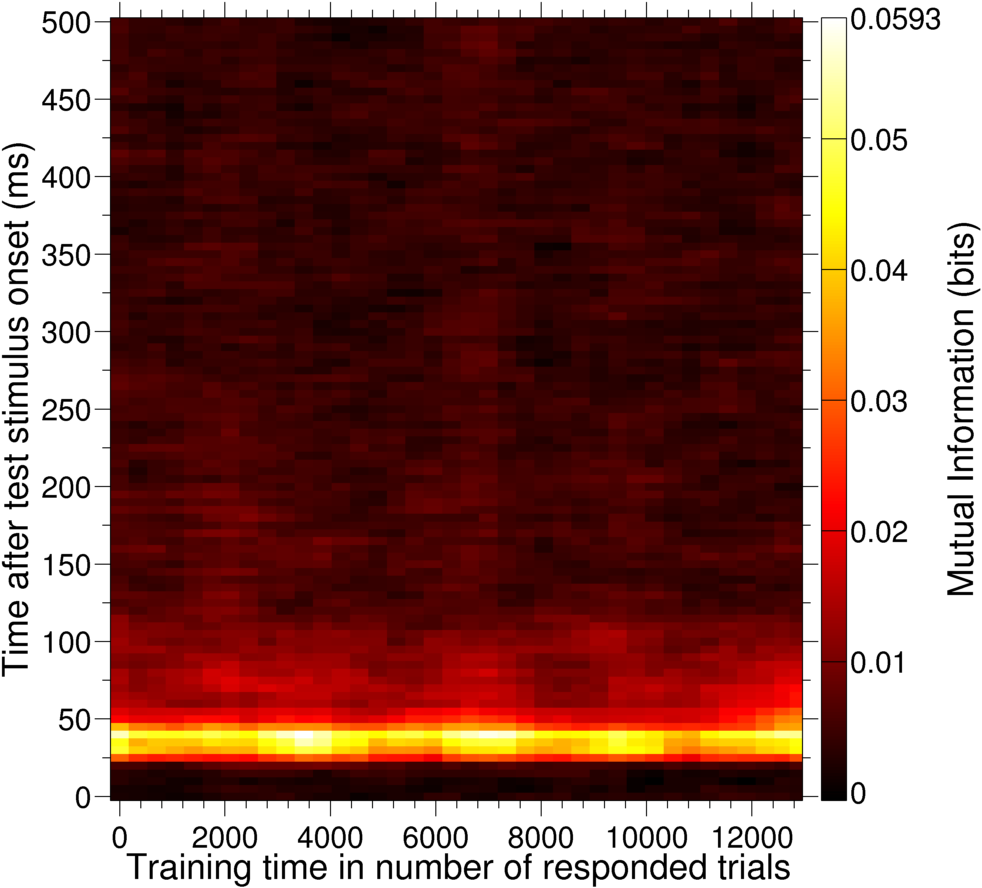
\includegraphics[scale=.25]{%
% % % ./figs/I_trialwise_blanco_v1_chmean23_s343-354,355.1,355.2,356-359_tp4_1bins_of_20ms_dr_pt_oc0_test_tc5-5-20,22-3-28,32,35-5-50,60,90_nt1400_ts350_rmvet1_rmvms0_pcolorhot_20120815T234452.png}
% % %         \caption{}
% % %         \label{fig:b1-1x20tp4ma}
% % %     \end{subfigure}
% % %     ~~
% % %     \begin{subfigure}[b]{0.5\linewidth}
% % %         \centering
% % %         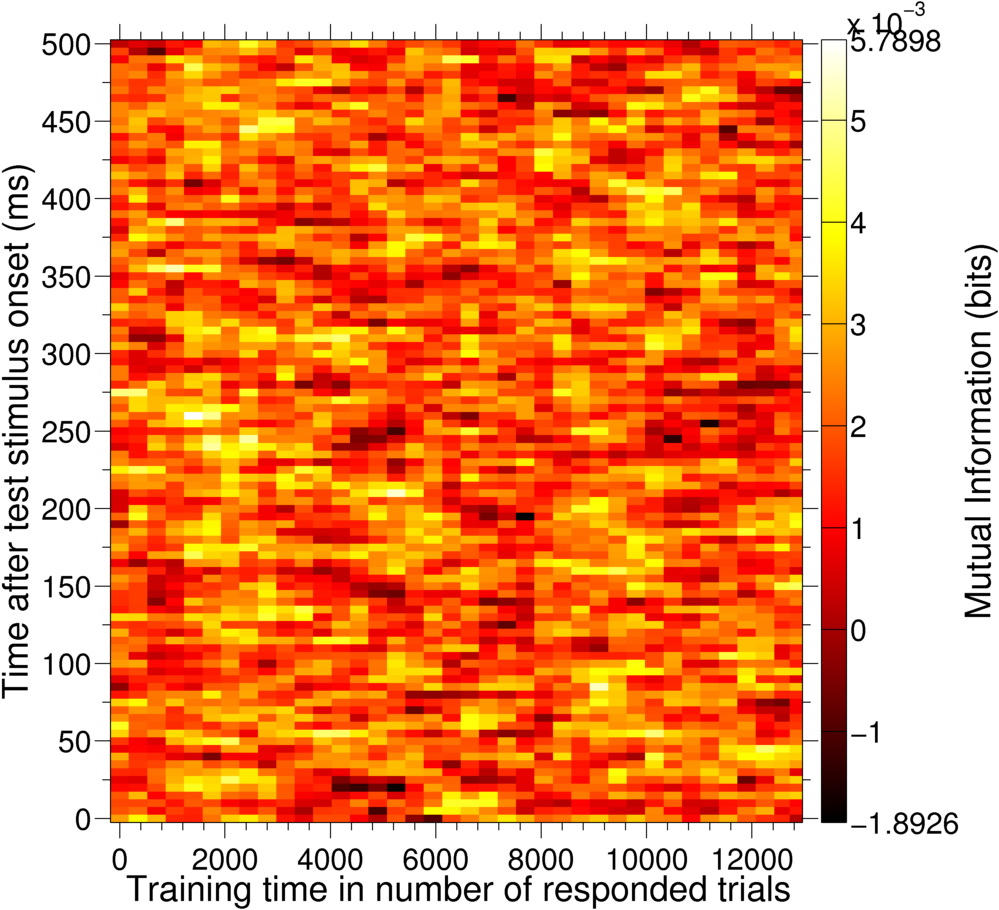
\includegraphics[scale=.25]{%
% % % ./figs/I_trialwise_blanco_v1_chmean23_s343-354,355.1,355.2,356-359_tp1_1bins_of_20ms_dr_pt_oc0_test_tc5-5-20,22-3-28,32,35-5-50,60,90_nt1400_ts350_rmvet1_rmvms0_pcolorhot_20120815T234326.png}
% % %         \caption{}
% % %         \label{fig:b1-1x20tp1ma}
% % %     \end{subfigure}
% % %     \\
% %     \begin{subfigure}[b]{0.5\linewidth}
% %         \centering
% %         \caption{}
% %         \label{fig:b1-1x20tp4}
% %         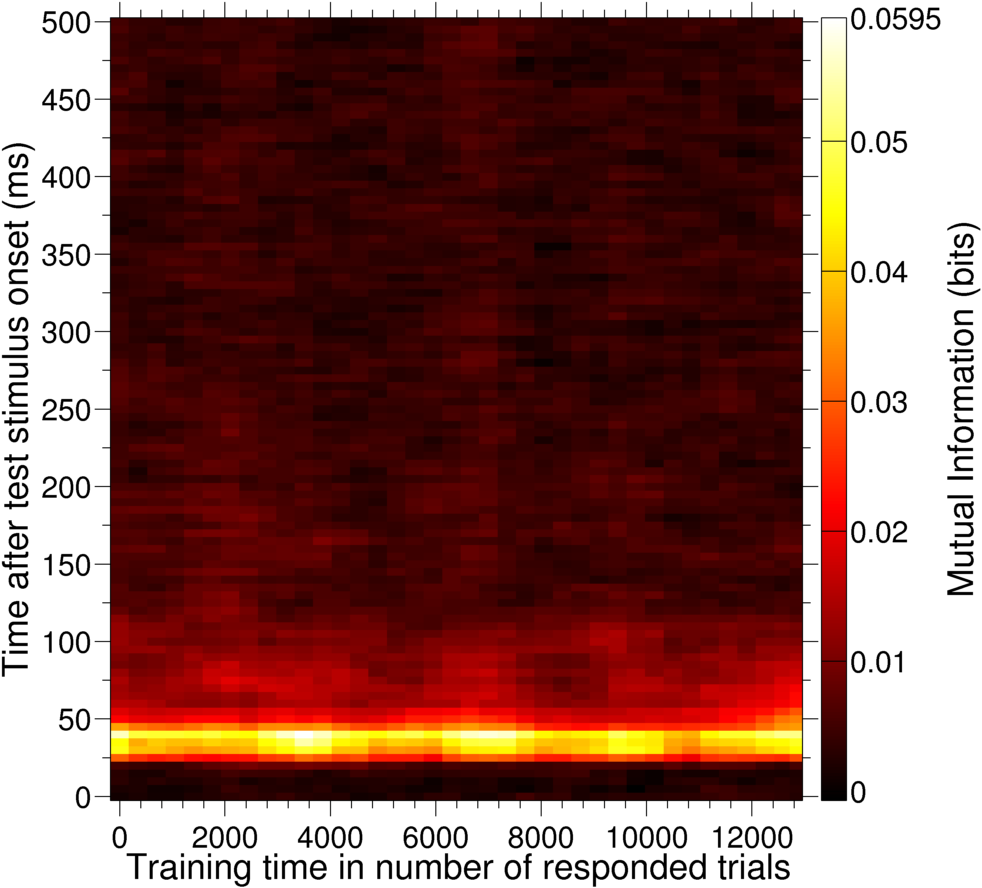
\includegraphics[scale=.25]{%
% % ./figs/I_trialwise_blanco_v1_chmean23_s343-354,355.1,355.2,356-359_tp4_1bins_of_20ms_dr_pt_oc0_test_tc5-5-20,22-3-28,32,35-5-50,60,90_nt1400_ts350_rmvet1_rmvms1_pcolorhot_20120815T234741.png}
% %     \end{subfigure}
% %     ~~
% %     \begin{subfigure}[b]{0.5\linewidth}
% %         \centering
% %         \caption{}
% %         \label{fig:b1-1x20tp1}
% %         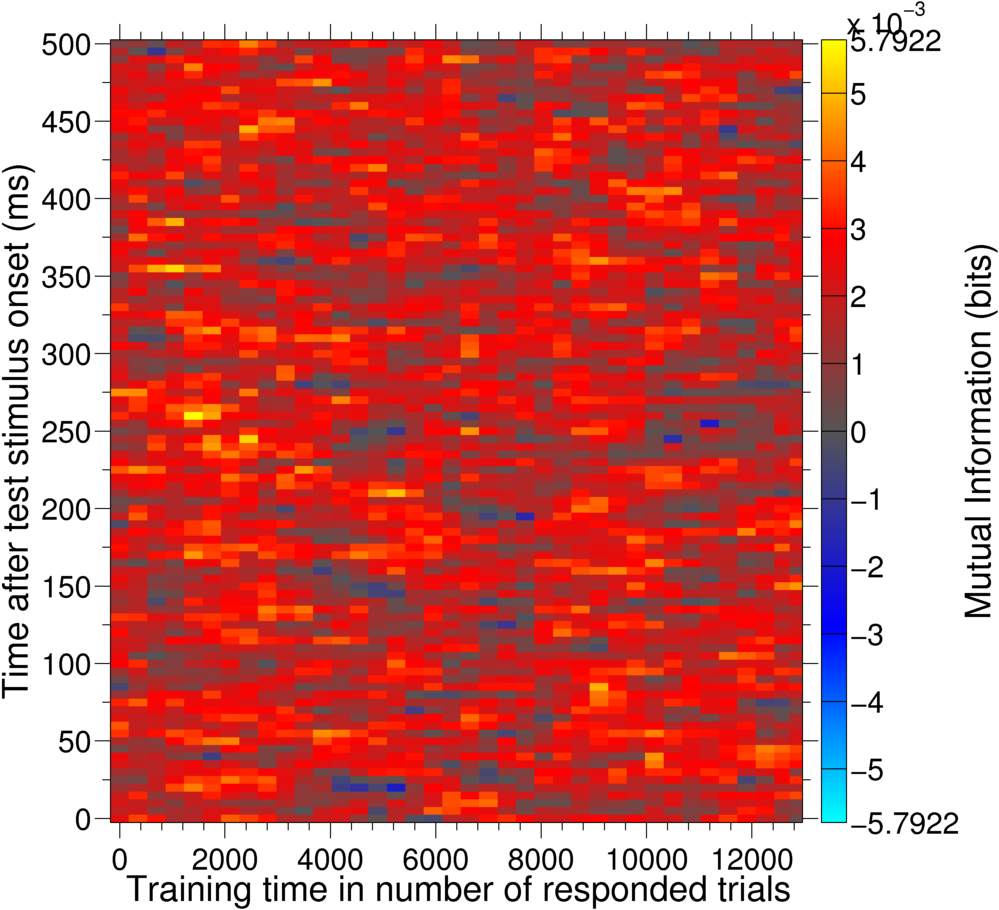
\includegraphics[scale=.25]{%
% % ./figs/I_trialwise_blanco_v1_chmean23_s343-354,355.1,355.2,356-359_tp1_1bins_of_20ms_dr_pt_oc0_test_tc5-5-20,22-3-28,32,35-5-50,60,90_nt1400_ts350_rmvet1_rmvms1_pcolorbp_20120816T175451.png}
% %     \end{subfigure}
% %     \\
% %     \begin{subfigure}[b]{0.5\linewidth}
% %         \centering
% %         \caption{}
% %         \label{fig:b1-5x4tp4}
% %         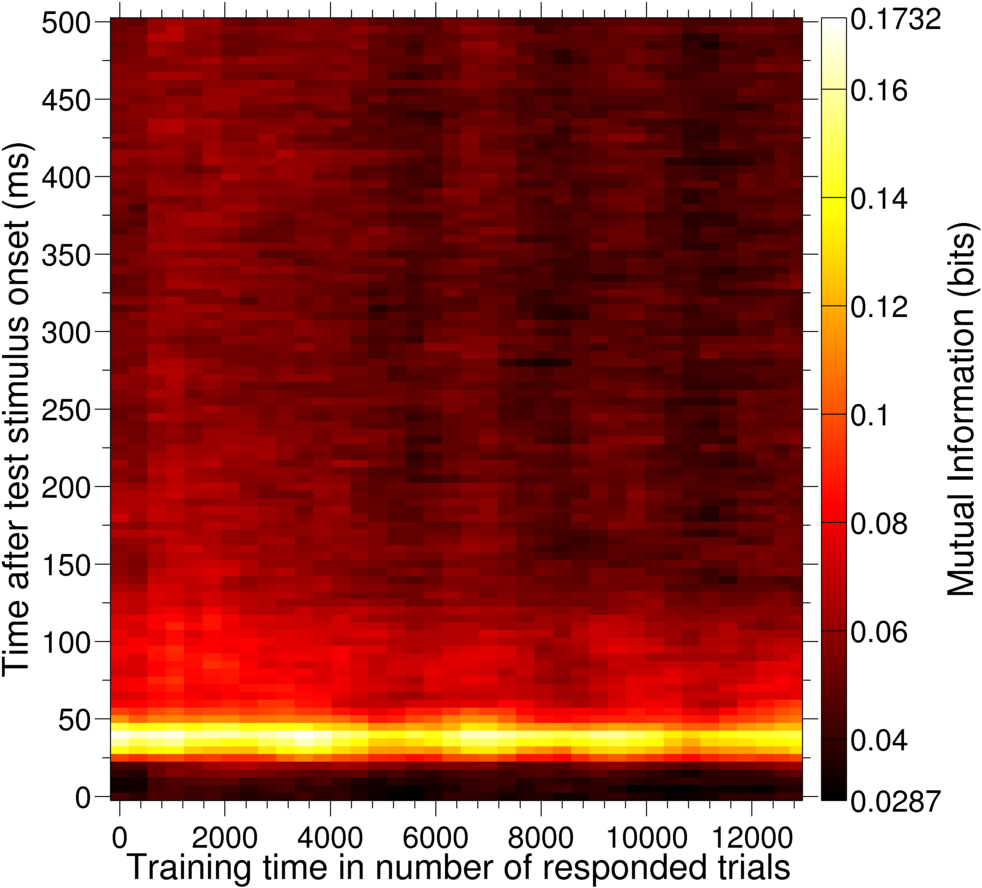
\includegraphics[scale=.25]{%
% % ./figs/I_trialwise_blanco_v1_chmean23_s343-354,355.1,355.2,356-359_tp4_5bins_of_4ms_dr_pt_oc0_test_tc5-5-20,22-3-28,32,35-5-50,60,90_nt1400_ts350_rmvet1_rmvms1_pcolorhot_20120815T234513.png}
% %     \end{subfigure}
% %     ~~
% %     \begin{subfigure}[b]{0.5\linewidth}
% %         \centering
% %         \caption{}
% %         \label{fig:b1-5x4tp1}
% %         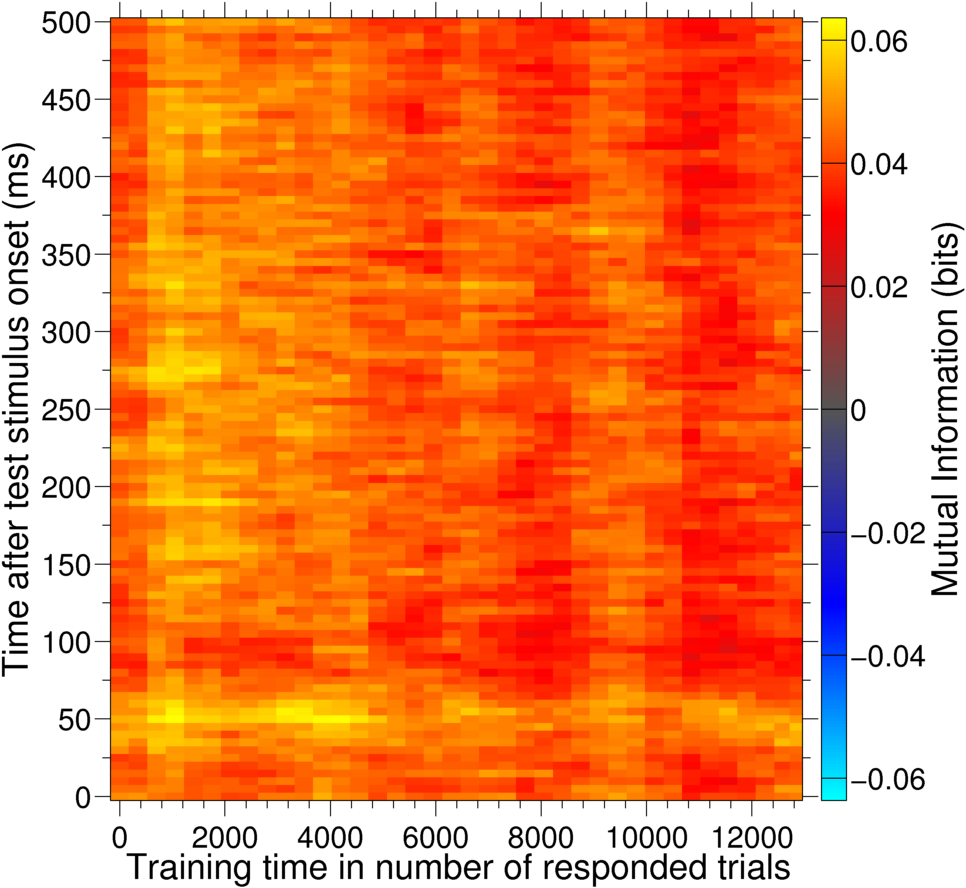
\includegraphics[scale=.25]{%
% % ./figs/I_trialwise_blanco_v1_chmean23_s343-354,355.1,355.2,356-359_tp1_5bins_of_4ms_dr_pt_oc0_test_tc5-5-20,22-3-28,32,35-5-50,60,90_nt1400_ts350_rmvet1_rmvms1_pcolorbp_20120816T175423.png}
% %     \end{subfigure}
% %     \caption{M1 V1: Mutual information between the test stimulus and \unit[20]{ms} of spiking activity, averaged across 23 channels.
% % The PT bias correction method was used in all estimates of the information, and the modification to the spiking data to remove the artifact as described in Sec.~\ref{sec:ma} was performed.
% % The neural code used in \ref{fig:b1-1x20tp4}, \ref{fig:b1-1x20tp1} is a spike count code, whilst in \ref{fig:b1-5x4tp4} and \ref{fig:b1-5x4tp1} it is a spike timing code where the \unit[20]{ms} window was subdivided into 5 bins each of \unit[4]{ms}.
% % In \ref{fig:b1-1x20tp4} and \ref{fig:b1-5x4tp4} the spike-train is taken from the test presentation part of the trial;
% % for \ref{fig:b1-1x20tp1} and \ref{fig:b1-5x4tp1} the spike-train is taken from spontaneous pre-stimulus activity.
% % The data is sampled in intervals of \unit[350]{trials} in the $x$-direction and \unit[5]{ms} in the $y$-direction, so there is significant correlation between any pair of pixels in the image with less than 4 pixels between them in either cartesian direction.
% % % In \ref{fig:b1-1x20tp4ma}, \ref{fig:b1-1x20tp4}, and \ref{fig:b1-5x4tp4}, the spike-train is taken from the test presentation part of the trial;
% % % for \ref{fig:b1-1x20tp1ma}, \ref{fig:b1-1x20tp1}, and \ref{fig:b1-5x4tp1}, the spike-train is taken from spontaneous pre-stimulus activity.
% % % In \ref{fig:b1-1x20tp4ma} and \ref{fig:b1-1x20tp1ma} no attempt was made to remove the monitor artifact from the raw data, whilst in the rest of the panels the data was modified to counter this as described in \ref{sec:ma}.
% % % \ref{fig:b1-1x20tp4ma}
% % % \ref{fig:b1-1x20tp1ma}
% % % \ref{fig:b1-1x20tp4}
% % % \ref{fig:b1-1x20tp1}
% % % \ref{fig:b1-5x4tp4}
% % % \ref{fig:b1-5x4tp1}
% % }
% %     \label{fig:b1-trialwise}
% % \end{figure}


% ./figs/I_trialwise_jack_v1_chmean25_s51-72_tp4_1bins_of_20ms_dr_pt_oc0_test_tc5-5-20,22-3-28,32,35-5-50,60,90_nt1400_ts350_rmvet1_rmvms0_pcolorhot_20120815T234410.png
% ./figs/I_trialwise_jack_v1_chmean25_s51-72_tp1_1bins_of_20ms_dr_pt_oc0_test_tc5-5-20,22-3-28,32,35-5-50,60,90_nt1400_ts350_rmvet1_rmvms0_pcolorhot_20120815T234245.png
% ./figs/I_trialwise_jack_v1_chmean25_s51-72_tp4_1bins_of_20ms_dr_pt_oc0_test_tc5-5-20,22-3-28,32,35-5-50,60,90_nt1400_ts350_rmvet1_rmvms1_pcolorhot_20120815T234701.png
% ./figs/I_trialwise_jack_v1_chmean25_s51-72_tp1_1bins_of_20ms_dr_pt_oc0_test_tc5-5-20,22-3-28,32,35-5-50,60,90_nt1400_ts350_rmvet1_rmvms1_pcolorbp_20120816T175411.png
% ./figs/I_trialwise_jack_v1_chmean25_s51-72_tp4_5bins_of_4ms_dr_pt_oc0_test_tc5-5-20,22-3-28,32,35-5-50,60,90_nt1400_ts350_rmvet1_rmvms1_pcolorhot_20120815T234434.png
% ./figs/I_trialwise_jack_v1_chmean25_s51-72_tp1_5bins_of_4ms_dr_pt_oc0_test_tc5-5-20,22-3-28,32,35-5-50,60,90_nt1400_ts350_rmvet1_rmvms1_pcolorbp_20120816T175343.png

% % \begin{figure}[htbp]
% % %     \begin{subfigure}[b]{0.5\linewidth}
% % %         \centering
% % %         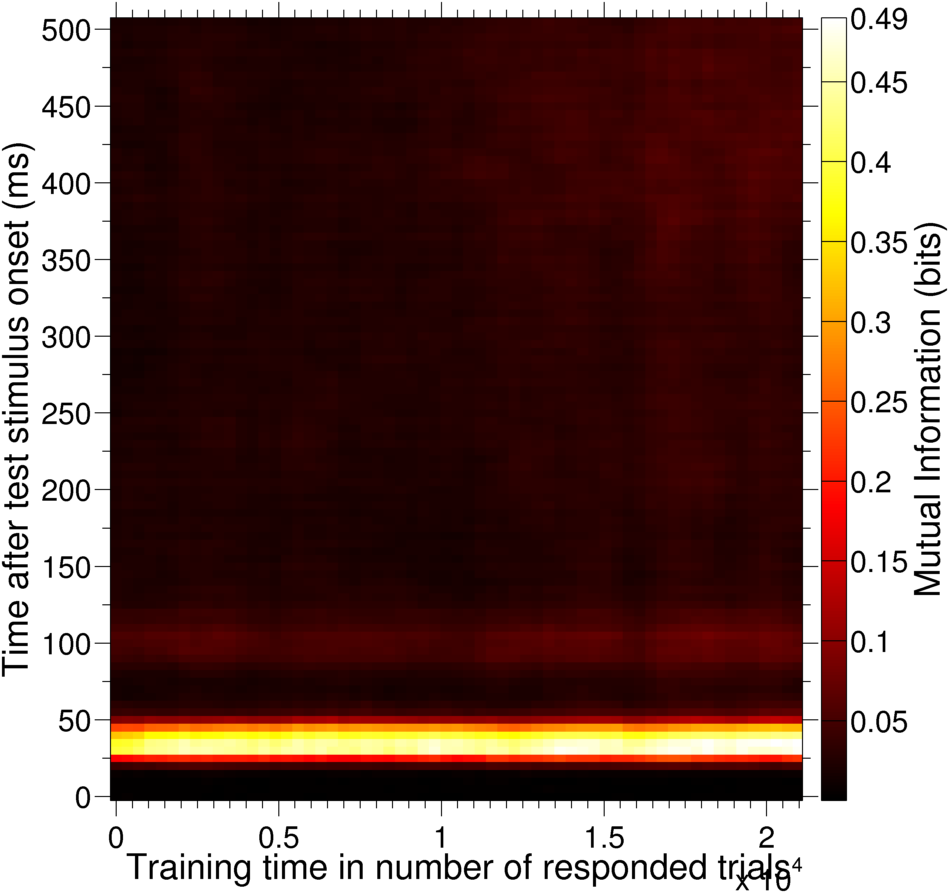
\includegraphics[scale=.25]{%
% % % ./figs/I_trialwise_jack_v1_chmean25_s51-72_tp4_1bins_of_20ms_dr_pt_oc0_test_tc5-5-20,22-3-28,32,35-5-50,60,90_nt1400_ts350_rmvet1_rmvms0_pcolorhot_20120815T234410.png}
% % %         \caption{}
% % %         \label{fig:j1-1x20tp4ma}
% % %     \end{subfigure}
% % %     ~~
% % %     \begin{subfigure}[b]{0.5\linewidth}
% % %         \centering
% % %         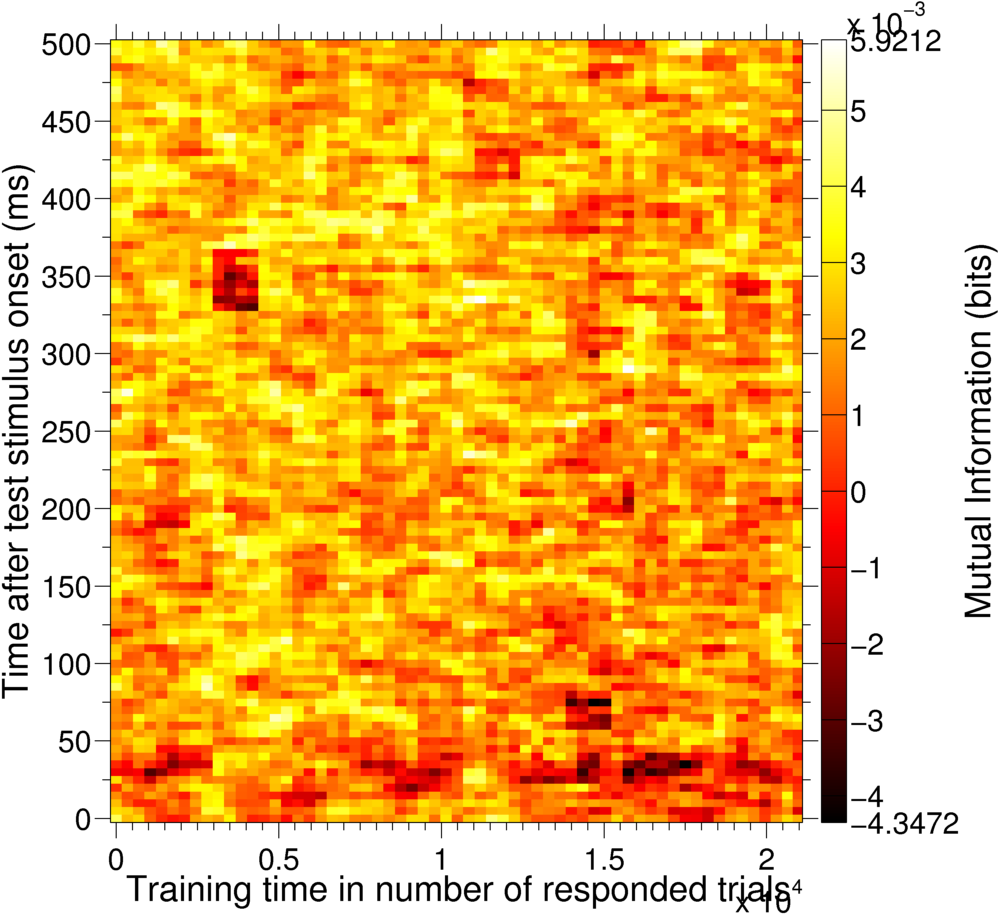
\includegraphics[scale=.25]{%
% % % ./figs/I_trialwise_jack_v1_chmean25_s51-72_tp1_1bins_of_20ms_dr_pt_oc0_test_tc5-5-20,22-3-28,32,35-5-50,60,90_nt1400_ts350_rmvet1_rmvms0_pcolorhot_20120815T234245.png}
% % %         \caption{}
% % %         \label{fig:j1-1x20tp1ma}
% % %     \end{subfigure}
% % %     \\
% %     \begin{subfigure}[b]{0.5\linewidth}
% %         \centering
% %         \caption{}
% %         \label{fig:j1-1x20tp4}
% %         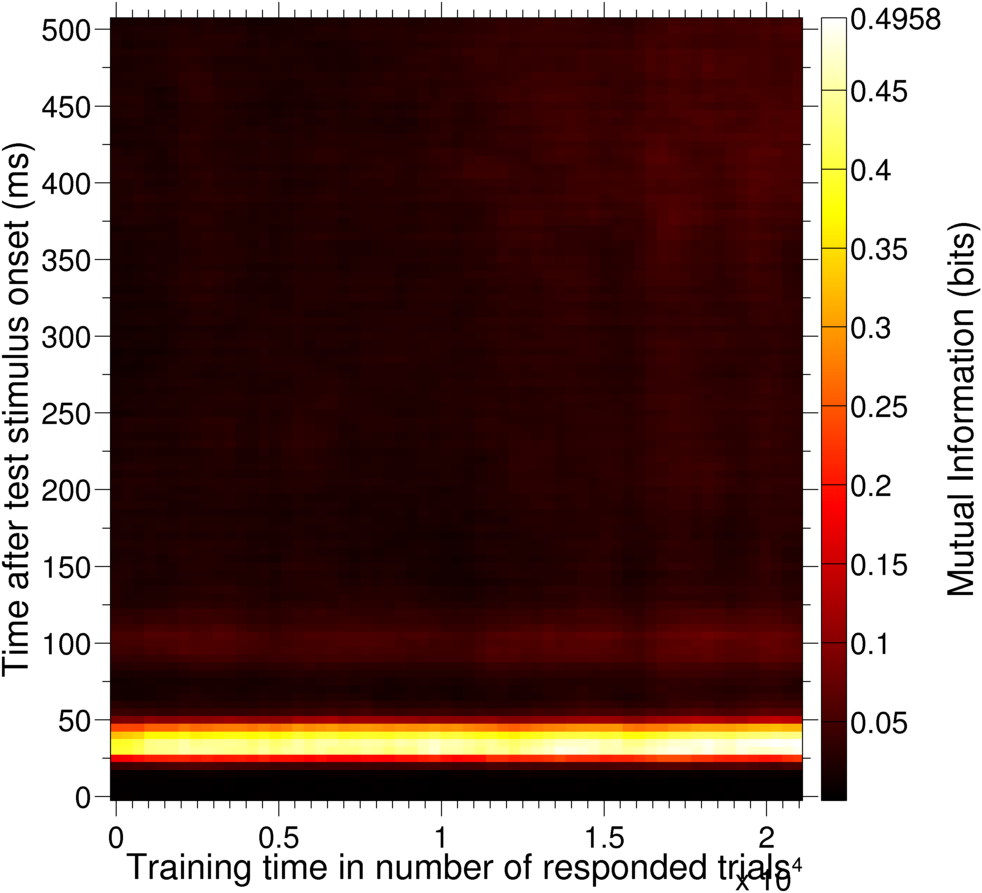
\includegraphics[scale=.25]{%
% % ./figs/I_trialwise_jack_v1_chmean25_s51-72_tp4_1bins_of_20ms_dr_pt_oc0_test_tc5-5-20,22-3-28,32,35-5-50,60,90_nt1400_ts350_rmvet1_rmvms1_pcolorhot_20120815T234701.png}
% %     \end{subfigure}
% %     ~~
% %     \begin{subfigure}[b]{0.5\linewidth}
% %         \centering
% %         \caption{}
% %         \label{fig:j1-1x20tp1}
% %         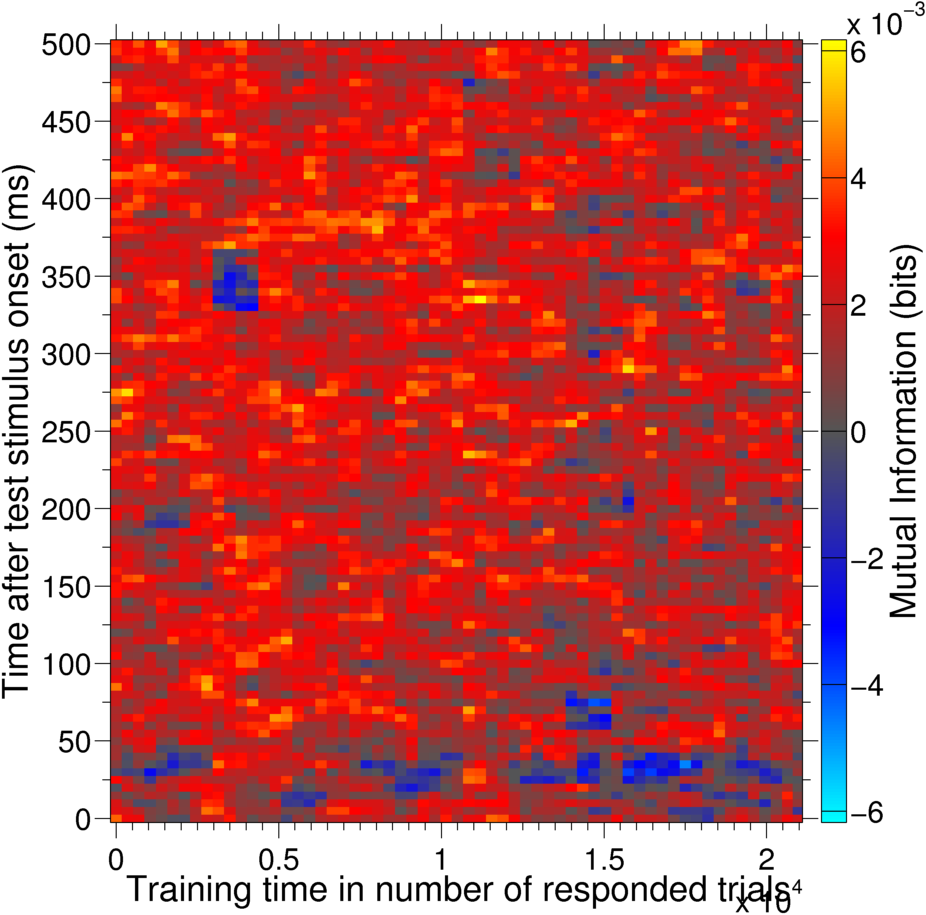
\includegraphics[scale=.25]{%
% % ./figs/I_trialwise_jack_v1_chmean25_s51-72_tp1_1bins_of_20ms_dr_pt_oc0_test_tc5-5-20,22-3-28,32,35-5-50,60,90_nt1400_ts350_rmvet1_rmvms1_pcolorbp_20120816T175411.png}
% %     \end{subfigure}
% %     \\
% %     \begin{subfigure}[b]{0.5\linewidth}
% %         \centering
% %         \caption{}
% %         \label{fig:j1-5x4tp4}
% %         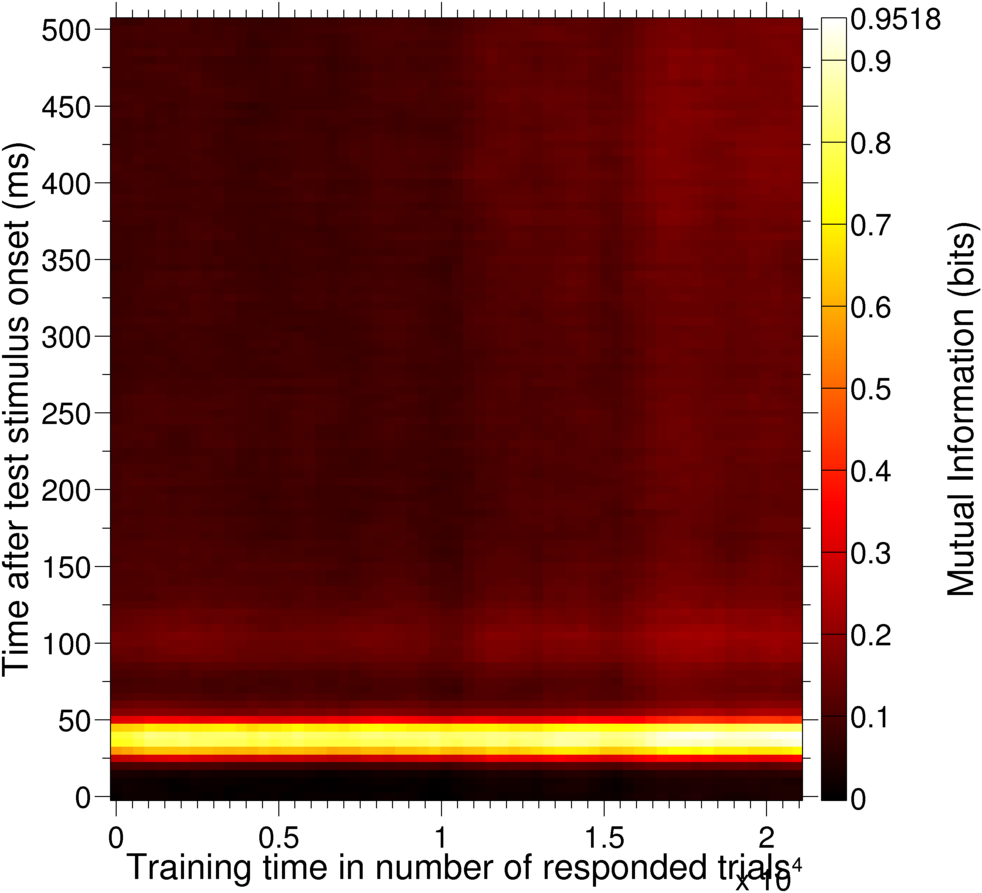
\includegraphics[scale=.25]{%
% % ./figs/I_trialwise_jack_v1_chmean25_s51-72_tp4_5bins_of_4ms_dr_pt_oc0_test_tc5-5-20,22-3-28,32,35-5-50,60,90_nt1400_ts350_rmvet1_rmvms1_pcolorhot_20120815T234434.png}
% %     \end{subfigure}
% %     ~~
% %     \begin{subfigure}[b]{0.5\linewidth}
% %         \centering
% %         \caption{}
% %         \label{fig:j1-5x4tp1}
% %         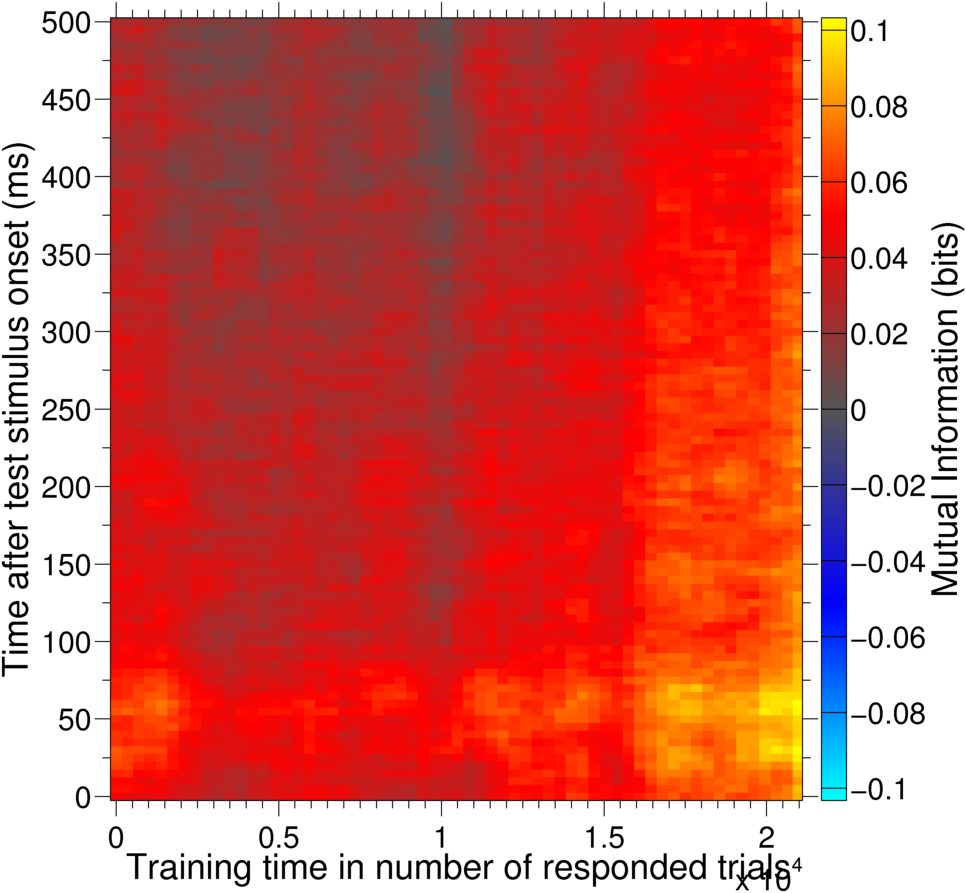
\includegraphics[scale=.25]{%
% % ./figs/I_trialwise_jack_v1_chmean25_s51-72_tp1_5bins_of_4ms_dr_pt_oc0_test_tc5-5-20,22-3-28,32,35-5-50,60,90_nt1400_ts350_rmvet1_rmvms1_pcolorbp_20120816T175343.png}
% %     \end{subfigure}
% %     \caption{M2 V1: Mutual information between the test stimulus and \unit[20]{ms} of spiking activity, averaged across 25 channels.
% % The PT bias correction method was used in all estimates of the information.
% % Panels \ref{fig:j1-1x20tp4}--\ref{fig:j1-5x4tp1} are the same as for Fig.~\ref{fig:b1-trialwise}.
% % % The neural code used in \ref{fig:j1-1x20tp4ma}--\ref{fig:j1-1x20tp1} is a spike count code, whilst in \ref{fig:j1-5x4tp4}, \ref{fig:j1-5x4tp1} it is a spike timing code where the \unit[20]{ms} window was subdivided into 5 bins each of \unit[4]{ms}.
% % % In \ref{fig:j1-1x20tp4ma}, \ref{fig:j1-1x20tp4}, and \ref{fig:j1-5x4tp4}, the spike-train is taken from the test presentation part of the trial;
% % % for \ref{fig:j1-1x20tp1ma}, \ref{fig:j1-1x20tp1}, and \ref{fig:j1-5x4tp1}, the spike-train is taken from spontaneous pre-stimulus activity.
% % % In \ref{fig:j1-1x20tp4ma} and \ref{fig:j1-1x20tp1ma} no attempt was made to remove the monitor artifact from the raw data, whilst in the rest of the panels the data was modified to counter this as described in \ref{sec:ma}.
% % % \ref{fig:j1-1x20tp4ma}
% % % \ref{fig:j1-1x20tp1ma}
% % % \ref{fig:j1-1x20tp4}
% % % \ref{fig:j1-1x20tp1}
% % % \ref{fig:j1-5x4tp4}
% % % \ref{fig:j1-5x4tp1}
% % }
% %     \label{fig:j1-trialwise}
% % \end{figure}

% ./figs/I_trialwise_blanco_v4_chmean31_s307,308,311,313,314,317,318,320,321,329-341_tp4_1bins_of_20ms_dr_pt_oc0_test_tc10-5-25,27-29,31-33,35,40-10-60_nt1400_ts350_rmvet1_rmvms0_pcolorhot_20120815T234508.png
% ./figs/I_trialwise_blanco_v4_chmean31_s307,308,311,313,314,317,318,320,321,329-341_tp1_1bins_of_20ms_dr_pt_oc0_test_tc10-5-25,27-29,31-33,35,40-10-60_nt1400_ts350_rmvet1_rmvms0_pcolorhot_20120815T234341.png
% ./figs/I_trialwise_blanco_v4_chmean31_s307,308,311,313,314,317,318,320,321,329-341_tp4_1bins_of_20ms_dr_pt_oc0_test_tc10-5-25,27-29,31-33,35,40-10-60_nt1400_ts350_rmvet1_rmvms1_pcolorhot_20120815T234756.png
% ./figs/I_trialwise_blanco_v4_chmean31_s307,308,311,313,314,317,318,320,321,329-341_tp1_1bins_of_20ms_dr_pt_oc0_test_tc10-5-25,27-29,31-33,35,40-10-60_nt1400_ts350_rmvet1_rmvms1_pcolorbp_20120816T175507.png
% ./figs/I_trialwise_blanco_v4_chmean31_s307,308,311,313,314,317,318,320,321,329-341_tp4_5bins_of_4ms_dr_pt_oc0_test_tc10-5-25,27-29,31-33,35,40-10-60_nt1400_ts350_rmvet1_rmvms1_pcolorhot_20120815T234528.png
% ./figs/I_trialwise_blanco_v4_chmean31_s307,308,311,313,314,317,318,320,321,329-341_tp1_5bins_of_4ms_dr_pt_oc0_test_tc10-5-25,27-29,31-33,35,40-10-60_nt1400_ts350_rmvet1_rmvms1_pcolorbp_20120816T175438.png

% % \cleartoevenpage

% % \begin{figure}[htbp]
% % %     \begin{subfigure}[b]{0.5\linewidth}
% % %         \centering
% % %         \includegraphics[scale=.25]{%
% % % ./figs/I_trialwise_blanco_v4_chmean31_s307,308,311,313,314,317,318,320,321,329-341_tp4_1bins_of_20ms_dr_pt_oc0_test_tc10-5-25,27-29,31-33,35,40-10-60_nt1400_ts350_rmvet1_rmvms0_pcolorhot_20120815T234508.png}
% % %         \caption{}
% % %         \label{fig:b4-1x20tp4ma}
% % %     \end{subfigure}
% % %     ~~
% % %     \begin{subfigure}[b]{0.5\linewidth}
% % %         \centering
% % %         \includegraphics[scale=.25]{%
% % % ./figs/I_trialwise_blanco_v4_chmean31_s307,308,311,313,314,317,318,320,321,329-341_tp1_1bins_of_20ms_dr_pt_oc0_test_tc10-5-25,27-29,31-33,35,40-10-60_nt1400_ts350_rmvet1_rmvms0_pcolorhot_20120815T234341.png}
% % %         \caption{}
% % %         \label{fig:b4-1x20tp1ma}
% % %     \end{subfigure}
% % %     \\
% %     \begin{subfigure}[b]{0.5\linewidth}
% %         \centering
% %         \caption{}
% %         \label{fig:b4-1x20tp4}
% %         \includegraphics[scale=.25]{%
% % ./figs/I_trialwise_blanco_v4_chmean31_s307,308,311,313,314,317,318,320,321,329-341_tp4_1bins_of_20ms_dr_pt_oc0_test_tc10-5-25,27-29,31-33,35,40-10-60_nt1400_ts350_rmvet1_rmvms1_pcolorhot_20120815T234756.png}
% %     \end{subfigure}
% %     ~~
% %     \begin{subfigure}[b]{0.5\linewidth}
% %         \centering
% %         \caption{}
% %         \label{fig:b4-1x20tp1}
% %         \includegraphics[scale=.25]{%
% % ./figs/I_trialwise_blanco_v4_chmean31_s307,308,311,313,314,317,318,320,321,329-341_tp1_1bins_of_20ms_dr_pt_oc0_test_tc10-5-25,27-29,31-33,35,40-10-60_nt1400_ts350_rmvet1_rmvms1_pcolorbp_20120816T175507.png}
% %     \end{subfigure}
% %     \\
% %     \begin{subfigure}[b]{0.5\linewidth}
% %         \centering
% %         \caption{}
% %         \label{fig:b4-5x4tp4}
% %         \includegraphics[scale=.25]{%
% % ./figs/I_trialwise_blanco_v4_chmean31_s307,308,311,313,314,317,318,320,321,329-341_tp4_5bins_of_4ms_dr_pt_oc0_test_tc10-5-25,27-29,31-33,35,40-10-60_nt1400_ts350_rmvet1_rmvms1_pcolorhot_20120815T234528.png}
% %     \end{subfigure}
% %     ~~
% %     \begin{subfigure}[b]{0.5\linewidth}
% %         \centering
% %         \caption{}
% %         \label{fig:b4-5x4tp1}
% %         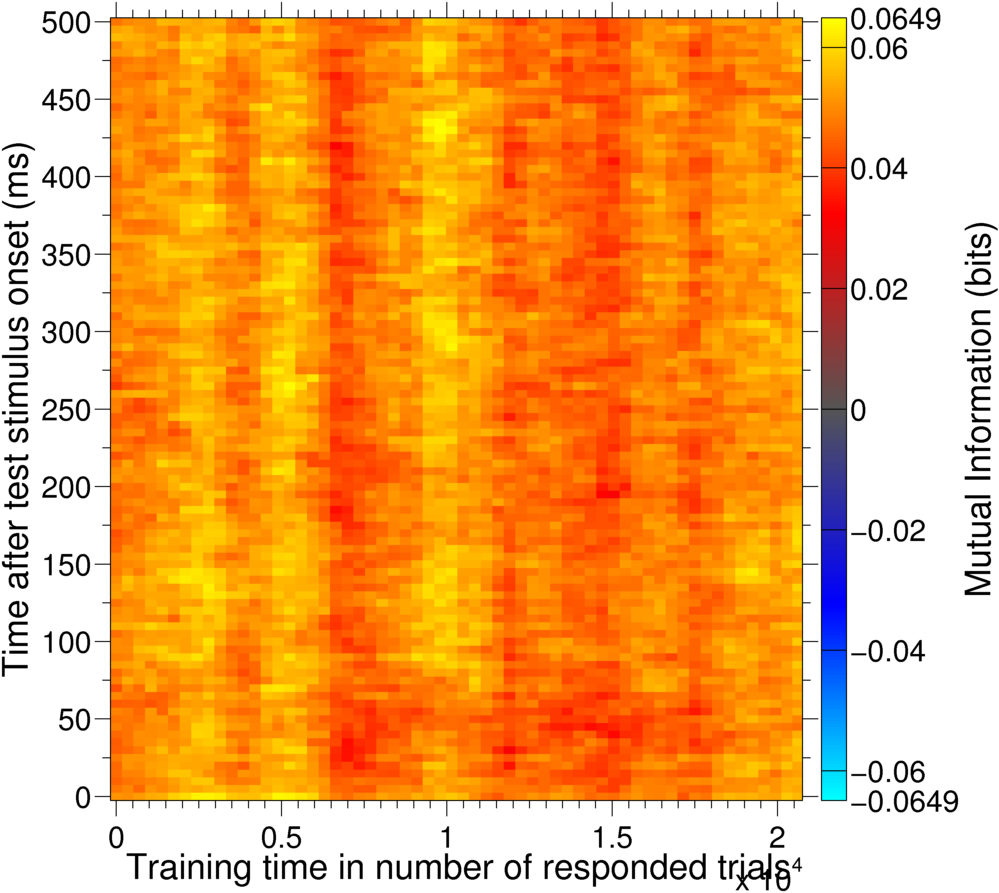
\includegraphics[scale=.25]{%
% % ./figs/I_trialwise_blanco_v4_chmean31_s307,308,311,313,314,317,318,320,321,329-341_tp1_5bins_of_4ms_dr_pt_oc0_test_tc10-5-25,27-29,31-33,35,40-10-60_nt1400_ts350_rmvet1_rmvms1_pcolorbp_20120816T175438.png}
% %     \end{subfigure}
% %     \caption{M1 V4: Mutual information between the test stimulus and \unit[20]{ms} of spiking activity, averaged across 30 channels.
% % The PT bias correction method was used in all estimates of the information.
% % Panels \ref{fig:b4-1x20tp4}--\ref{fig:b4-5x4tp1} are the same as for Fig.~\ref{fig:b1-trialwise}.
% % % The neural code used in \ref{fig:b4-1x20tp4ma}--\ref{fig:b4-1x20tp1} is a spike count code, whilst in \ref{fig:b4-5x4tp4}, \ref{fig:b4-5x4tp1} it is a spike timing code where the \unit[20]{ms} window was subdivided into 5 bins each of \unit[4]{ms}.
% % % In \ref{fig:b4-1x20tp4ma}, \ref{fig:b4-1x20tp4}, and \ref{fig:b4-5x4tp4}, the spike-train is taken from the test presentation part of the trial;
% % % for \ref{fig:b4-1x20tp1ma}, \ref{fig:b4-1x20tp1}, and \ref{fig:b4-5x4tp1}, the spike-train is taken from spontaneous pre-stimulus activity.
% % % In \ref{fig:b4-1x20tp4ma} and \ref{fig:b4-1x20tp1ma} no attempt was made to remove the monitor artifact from the raw data, whilst in the rest of the panels the data was modified to counter this as described in \ref{sec:ma}.
% % % \ref{fig:b4-1x20tp4ma}
% % % \ref{fig:b4-1x20tp1ma}
% % % \ref{fig:b4-1x20tp4}
% % % \ref{fig:b4-1x20tp1}
% % % \ref{fig:b4-5x4tp4}
% % % \ref{fig:b4-5x4tp1}
% % }
% %     \label{fig:b4-trialwise}
% % \end{figure}



% ./figs/I_trialwise_jack_v4_chmean20_s24-49_tp4_1bins_of_20ms_dr_pt_oc0_test_tc10-5-25,27-29,31-33,35,40-10-60_nt1400_ts350_rmvet1_rmvms0_pcolorhot_20120815T234433.png
% ./figs/I_trialwise_jack_v4_chmean20_s24-49_tp1_1bins_of_20ms_dr_pt_oc0_test_tc10-5-25,27-29,31-33,35,40-10-60_nt1400_ts350_rmvet1_rmvms1_pcolorbp_20120816T175433.png
% ./figs/I_trialwise_jack_v4_chmean20_s24-49_tp4_1bins_of_20ms_dr_pt_oc0_test_tc10-5-25,27-29,31-33,35,40-10-60_nt1400_ts350_rmvet1_rmvms1_pcolorhot_20120815T234723.png
% ./figs/I_trialwise_jack_v4_chmean20_s24-49_tp1_1bins_of_20ms_dr_pt_oc0_test_tc10-5-25,27-29,31-33,35,40-10-60_nt1400_ts350_rmvet1_rmvms1_pcolorhot_20120815T234559.png
% ./figs/I_trialwise_jack_v4_chmean20_s24-49_tp4_5bins_of_4ms_dr_pt_oc0_test_tc10-5-25,27-29,31-33,35,40-10-60_nt1400_ts350_rmvet1_rmvms1_pcolorhot_20120815T234455.png
% ./figs/I_trialwise_jack_v4_chmean20_s24-49_tp1_5bins_of_4ms_dr_pt_oc0_test_tc10-5-25,27-29,31-33,35,40-10-60_nt1400_ts350_rmvet1_rmvms1_pcolorbp_20120816T175404.png

% % \begin{figure}[htbp]
% % %     \begin{subfigure}[b]{0.5\linewidth}
% % %         \centering
% % %         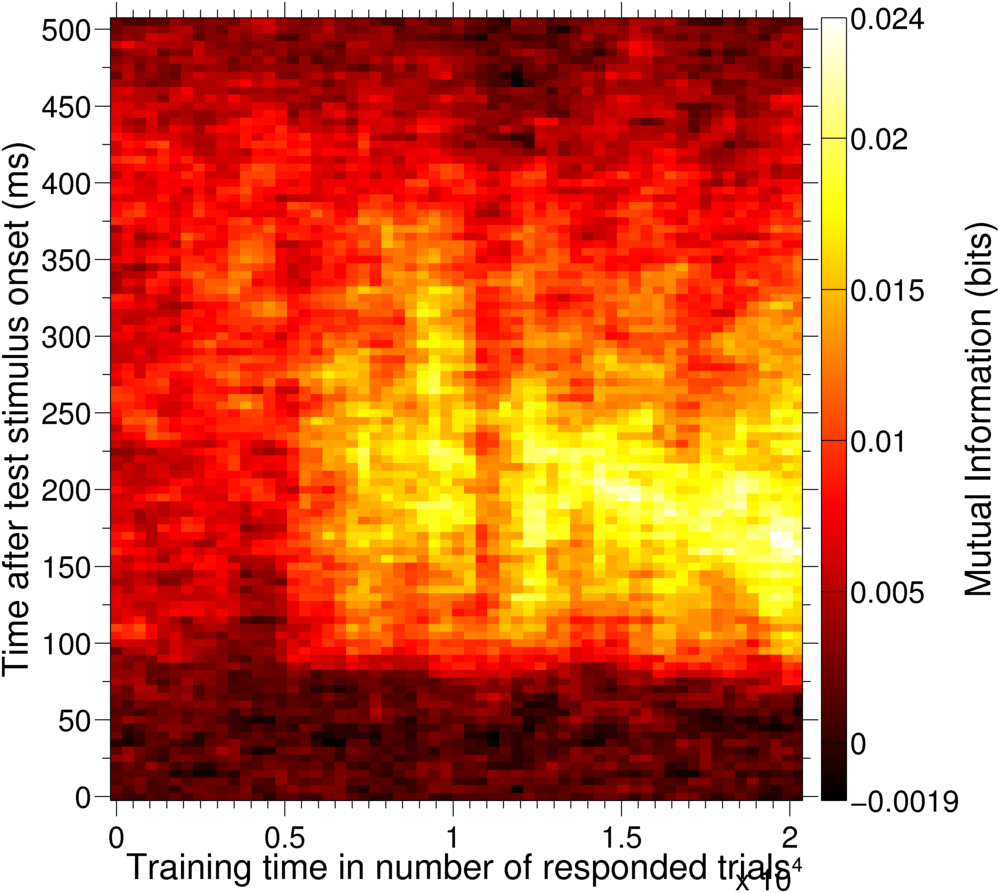
\includegraphics[scale=.25]{%
% % % ./figs/I_trialwise_jack_v4_chmean20_s24-49_tp4_1bins_of_20ms_dr_pt_oc0_test_tc10-5-25,27-29,31-33,35,40-10-60_nt1400_ts350_rmvet1_rmvms0_pcolorhot_20120815T234433.png}
% % %         \caption{}
% % %         \label{fig:j4-1x20tp4ma}
% % %     \end{subfigure}
% % %     ~~
% % %     \begin{subfigure}[b]{0.5\linewidth}
% % %         \centering
% % %         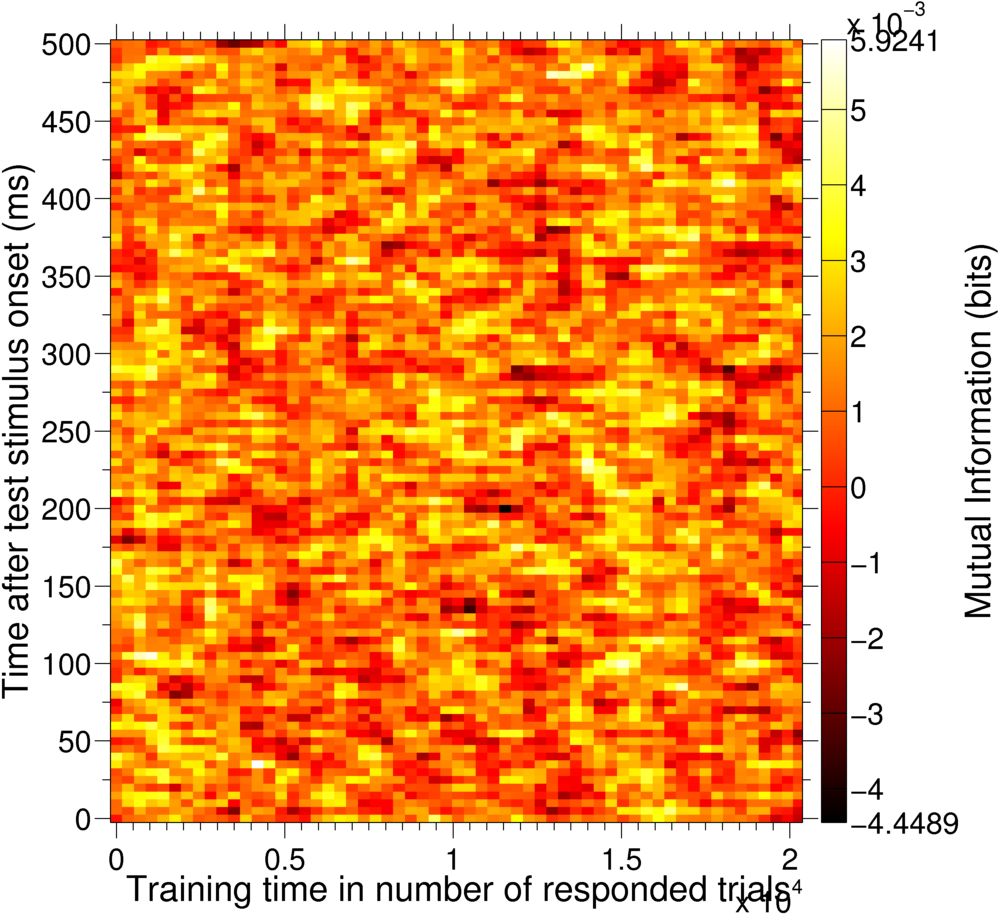
\includegraphics[scale=.25]{%
% % % ./figs/I_trialwise_jack_v4_chmean20_s24-49_tp1_1bins_of_20ms_dr_pt_oc0_test_tc10-5-25,27-29,31-33,35,40-10-60_nt1400_ts350_rmvet1_rmvms0_pcolorhot_20120815T234307.png}
% % %         \caption{}
% % %         \label{fig:j4-1x20tp1ma}
% % %     \end{subfigure}
% % %     \\
% %     \begin{subfigure}[b]{0.5\linewidth}
% %         \centering
% %         \caption{}
% %         \label{fig:j4-1x20tp4}
% %         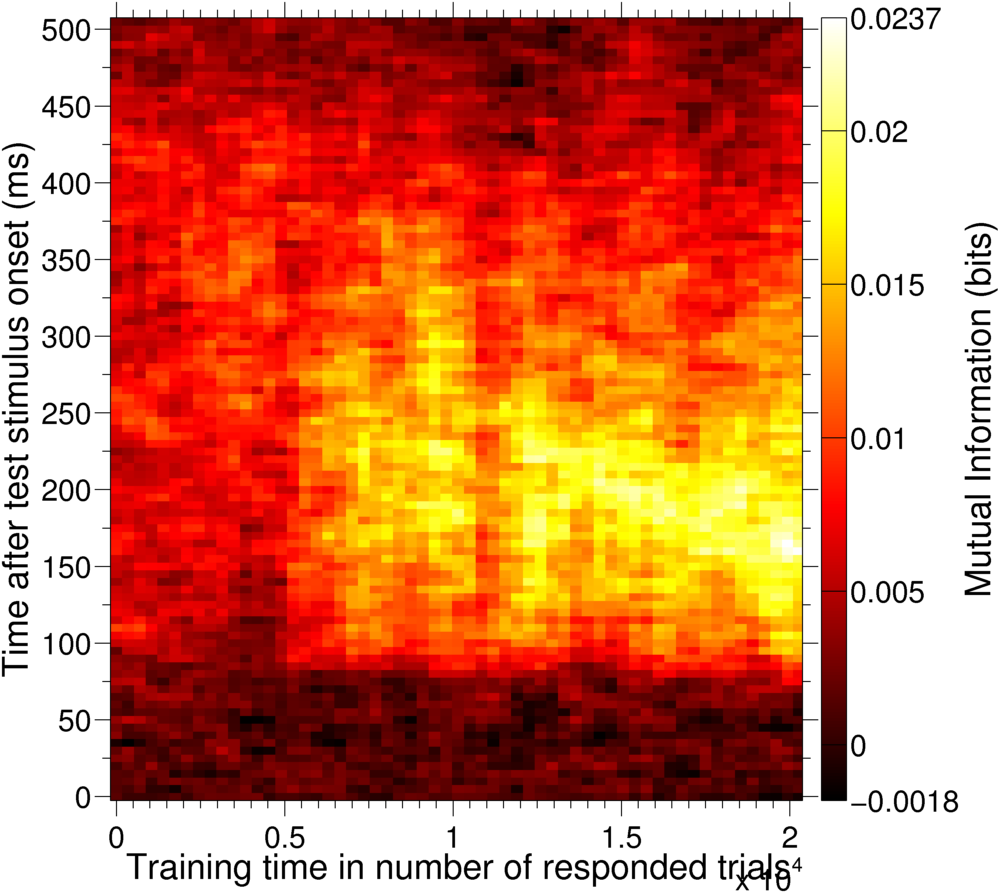
\includegraphics[scale=.25]{%
% % ./figs/I_trialwise_jack_v4_chmean20_s24-49_tp4_1bins_of_20ms_dr_pt_oc0_test_tc10-5-25,27-29,31-33,35,40-10-60_nt1400_ts350_rmvet1_rmvms1_pcolorhot_20120815T234723.png}
% %     \end{subfigure}
% %     ~~
% %     \begin{subfigure}[b]{0.5\linewidth}
% %         \centering
% %         \caption{}
% %         \label{fig:j4-1x20tp1}
% %         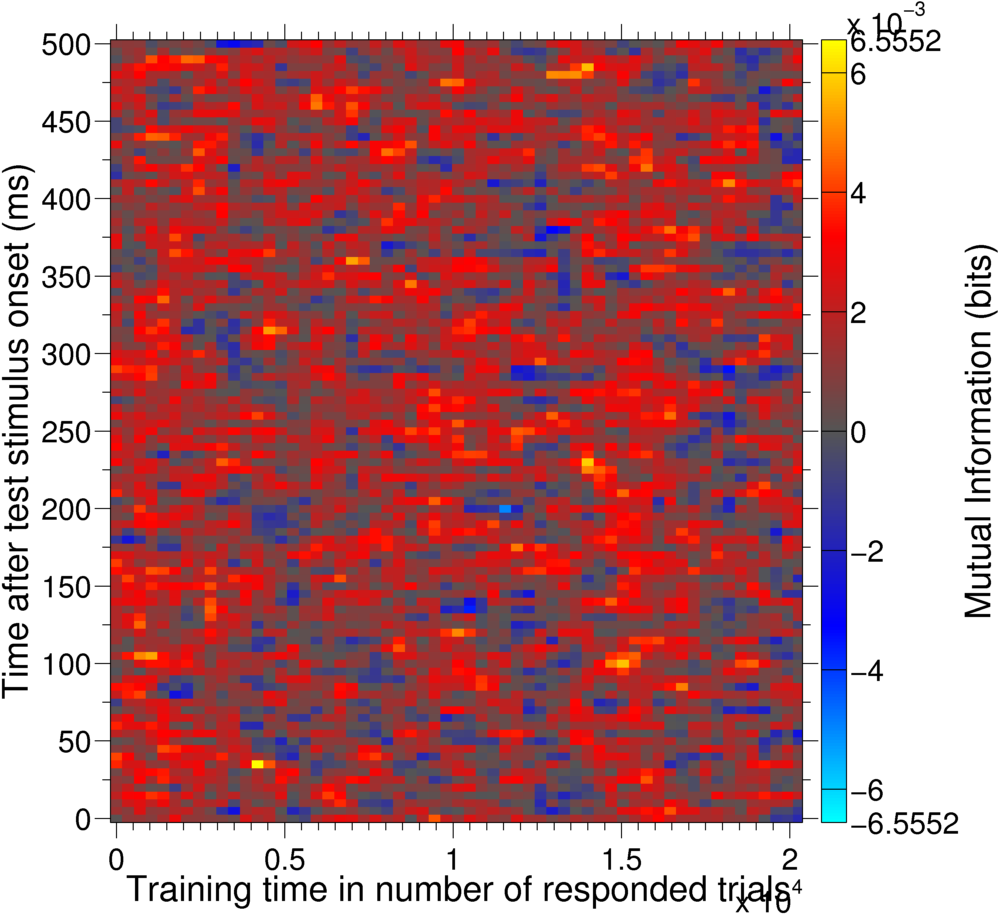
\includegraphics[scale=.25]{%
% % ./figs/I_trialwise_jack_v4_chmean20_s24-49_tp1_1bins_of_20ms_dr_pt_oc0_test_tc10-5-25,27-29,31-33,35,40-10-60_nt1400_ts350_rmvet1_rmvms1_pcolorbp_20120816T175433.png}
% %     \end{subfigure}
% %     \\
% %     \begin{subfigure}[b]{0.5\linewidth}
% %         \centering
% %         \caption{}
% %         \label{fig:j4-5x4tp4}
% %         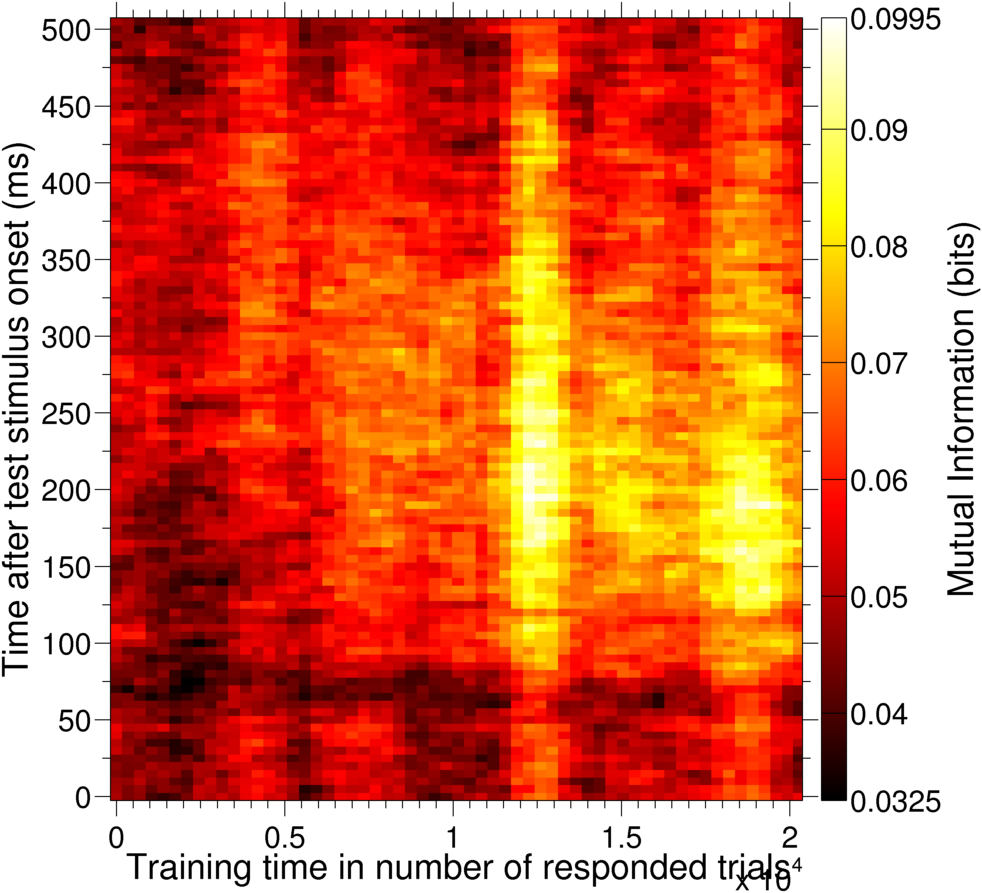
\includegraphics[scale=.25]{%
% % ./figs/I_trialwise_jack_v4_chmean20_s24-49_tp4_5bins_of_4ms_dr_pt_oc0_test_tc10-5-25,27-29,31-33,35,40-10-60_nt1400_ts350_rmvet1_rmvms1_pcolorhot_20120815T234455.png}
% %     \end{subfigure}
% %     ~~
% %     \begin{subfigure}[b]{0.5\linewidth}
% %         \centering
% %         \caption{}
% %         \label{fig:j4-5x4tp1}
% %         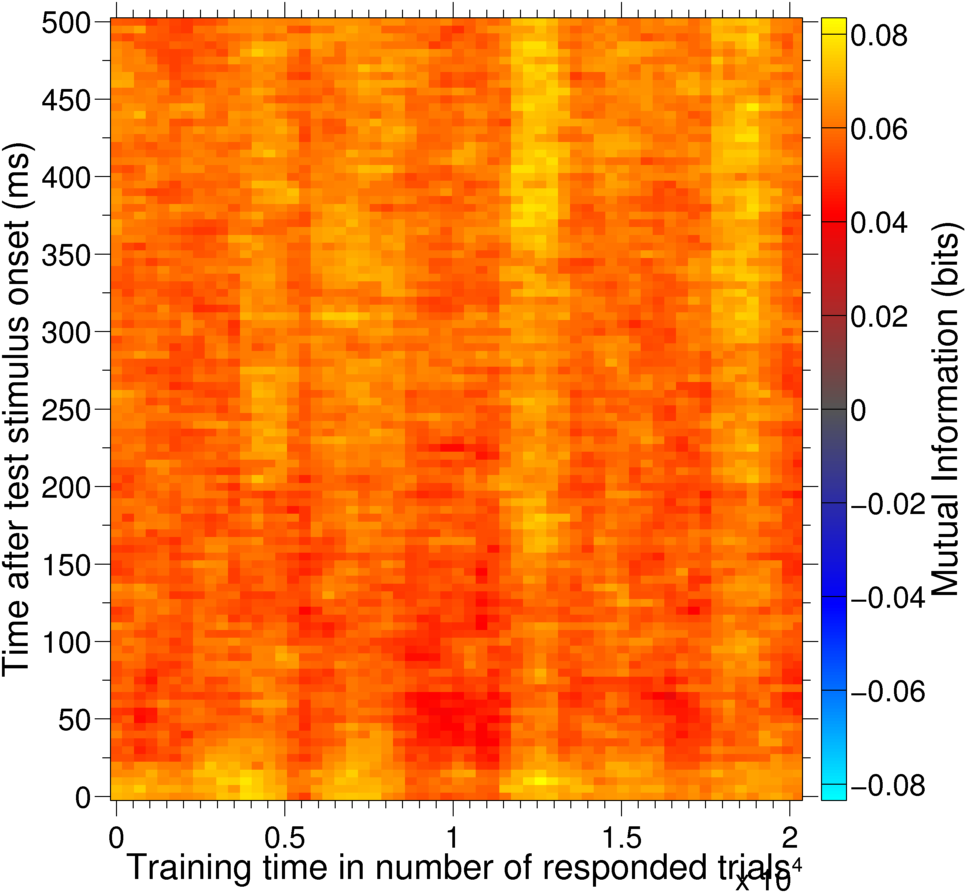
\includegraphics[scale=.25]{%
% % ./figs/I_trialwise_jack_v4_chmean20_s24-49_tp1_5bins_of_4ms_dr_pt_oc0_test_tc10-5-25,27-29,31-33,35,40-10-60_nt1400_ts350_rmvet1_rmvms1_pcolorbp_20120816T175404.png}
% %     \end{subfigure}
% %     \caption{M2 V4: Mutual information between the test stimulus and \unit[20]{ms} of spiking activity, averaged across 20 channels.
% % The PT bias correction method was used in all estimates of the information.
% % Panels \ref{fig:j4-1x20tp4}--\ref{fig:j4-5x4tp1} are the same as for Fig.~\ref{fig:b1-trialwise}.
% % % The neural code used in \ref{fig:j4-1x20tp4ma}--\ref{fig:j4-1x20tp1} is a spike count code, whilst in \ref{fig:j4-5x4tp4}, \ref{fig:j4-5x4tp1} it is a spike timing code where the \unit[20]{ms} window was subdivided into 5 bins each of \unit[4]{ms}.
% % % In \ref{fig:j4-1x20tp4ma}, \ref{fig:j4-1x20tp4}, and \ref{fig:j4-5x4tp4}, the spike-train is taken from the test presentation part of the trial;
% % % for \ref{fig:j4-1x20tp1ma}, \ref{fig:j4-1x20tp1}, and \ref{fig:j4-5x4tp1}, the spike-train is taken from spontaneous pre-stimulus activity.
% % % In \ref{fig:j4-1x20tp4ma} and \ref{fig:j4-1x20tp1ma} no attempt was made to remove the monitor artifact from the raw data, whilst in the rest of the panels the data was modified to counter this as described in \ref{sec:ma}.
% % % \ref{fig:j4-1x20tp4ma}
% % % \ref{fig:j4-1x20tp1ma}
% % % \ref{fig:j4-1x20tp4}
% % % \ref{fig:j4-1x20tp1}
% % % \ref{fig:j4-5x4tp4}
% % % \ref{fig:j4-5x4tp1}
% % }
% %     \label{fig:j4-trialwise}
% % \end{figure}

% 20, 30 and \unit[40]{ms} all tried. Mutual information increases as the duration increases as one would expect, but there is no other significant difference. Consequently only 20ms is shown in this section.

% More information with only correct trials used, but this could be due to differences in $P(S)$.

Turning our attention to the V4 results in Figs.~\ref{fig:b4-trialwise} and \ref{fig:j4-trialwise}, we can see the effect of the transient is present in M1's data (at the later start time of \unit[75]{ms}), but not in M2's. This is surprising because, looking at the rasters, in both animals there are some channels which exhibit a transient response and some which do not.

Similar to V1, it seems as if there is four times as much information in the timebinned code compared with the count code. However, there is much more information measured for the spontaneous activity data again. This is not reduced by increasing the number of trials either.

For the spike count code in M2, the spontaneous information is nearly distributed around 0, suggesting the bias has been all but removed and the data is of very high quality. For this animal, we can see a distinct increase in the information content with time, for both the spike count and timing codes. Simultaneously, there is a movement of the peak information to earlier times closer to the stimulus onset.

In M1, there is a small increase in the information content with time which may or may not significant. However, it is reassuring to see that this is not due to an improvement in the data with time, as the trend in the spontaneous activity information bias (Fig.~\ref{fig:j4-5x4tp1}) is a decrease with time.

%----------------------------------------------------------------------------------------------------------------------
\FloatBarrier
\subsubsection{Fine vs coarse contrast differences}

Comparing Figs.~\ref{fig:b1-1x20cc} and \ref{fig:j1-1x20cc} where the outer 6 contrasts are included with Figs.~\ref{fig:b1-1x20tp4} and \ref{fig:b1-1x20tp4} where all contrasts are included, it seems as if the amount of information has increased, which should not be possible. However, the difference will be due to the difference in trials contained in each of the analyses. In each case, an average of 100 trials per stimulus is used, but since the easier test conditions are presented less frequently, they are under-represented in Figs.~\ref{fig:b1-1x20tp4} and \ref{fig:b1-1x20tp4} (about 75 trials per stimulus). Obviously these are more discriminable, so the under-representation comparably reduces the information.

Looking at V1 (Fig.~\ref{fig:v1-fvc}), we observe there is much more information for M2 than M1, as we found before. The quality of the data seems to have severely hampered the analysis for M1, destroying the the fine differences in the data needed to evaluate the information contained about fine contrast differences (Fig.~\ref{fig:b1-1x20fc}).

Unsurprisingly, there is more information when considering the coarsely distinct contrasts than the finer differences, as the neural activity is bound to be more discriminable for these. For M2, there is a small upward trend again for both coarse and fine contrast differences, which may or may not be genuine.

% ./figs/I_trialwise_blanco_v1_chmean23_s343-354,355.1,355.2,356-359_tp4_1bins_of_20ms_dr_pt_oc0_test_tc5,15,22,40,50,90_nt600_ts150_rmvet1_rmvms1_pcolorhot_20120816T011936.png
% ./figs/I_trialwise_blanco_v1_chmean23_s343-354,355.1,355.2,356-359_tp4_1bins_of_20ms_dr_pt_oc0_test_tc22-3-28,32,35,40_nt600_ts150_rmvet1_rmvms1_pcolorhot_20120816T011920.png
% ./figs/I_trialwise_jack_v1_chmean25_s51-72_tp4_1bins_of_20ms_dr_pt_oc0_test_tc5,15,22,40,50,90_nt600_ts150_rmvet1_rmvms1_pcolorhot_20120816T011822.png
% ./figs/I_trialwise_jack_v1_chmean25_s51-72_tp4_1bins_of_20ms_dr_pt_oc0_test_tc22-3-28,32,35,40_nt600_ts150_rmvet1_rmvms1_pcolorhot_20120816T011800.png

% % \begin{figure}[htbp]
% %     \begin{subfigure}[b]{0.5\linewidth}
% %         \centering
% %         \caption{}
% %         \label{fig:b1-1x20cc}
% %         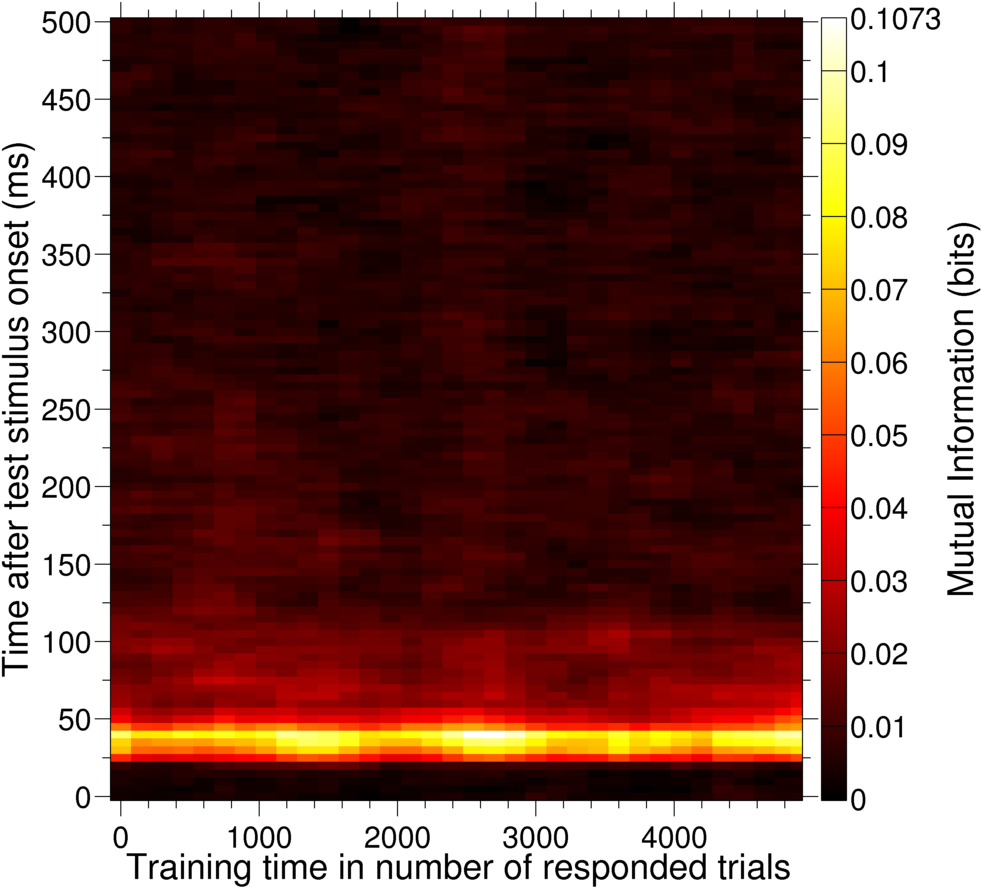
\includegraphics[scale=.25]{%
% % ./figs/I_trialwise_blanco_v1_chmean23_s343-354,355.1,355.2,356-359_tp4_1bins_of_20ms_dr_pt_oc0_test_tc5,15,22,40,50,90_nt600_ts150_rmvet1_rmvms1_pcolorhot_20120816T011936.png}
% %     \end{subfigure}
% %     ~~
% %     \begin{subfigure}[b]{0.5\linewidth}
% %         \centering
% %         \caption{}
% %         \label{fig:j1-1x20cc}
% %         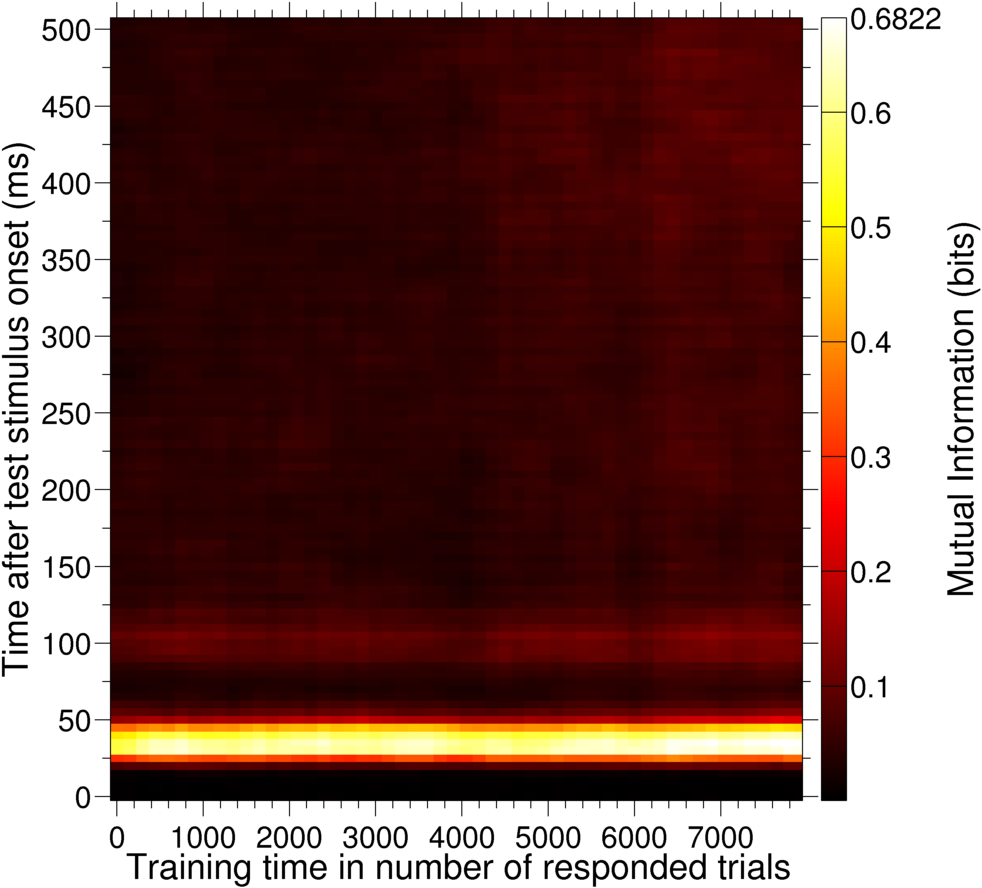
\includegraphics[scale=.25]{%
% % ./figs/I_trialwise_jack_v1_chmean25_s51-72_tp4_1bins_of_20ms_dr_pt_oc0_test_tc5,15,22,40,50,90_nt600_ts150_rmvet1_rmvms1_pcolorhot_20120816T011822.png}
% %     \end{subfigure}
% %     \\
% %     \begin{subfigure}[b]{0.5\linewidth}
% %         \centering
% %         \caption{}
% %         \label{fig:b1-1x20fc}
% %         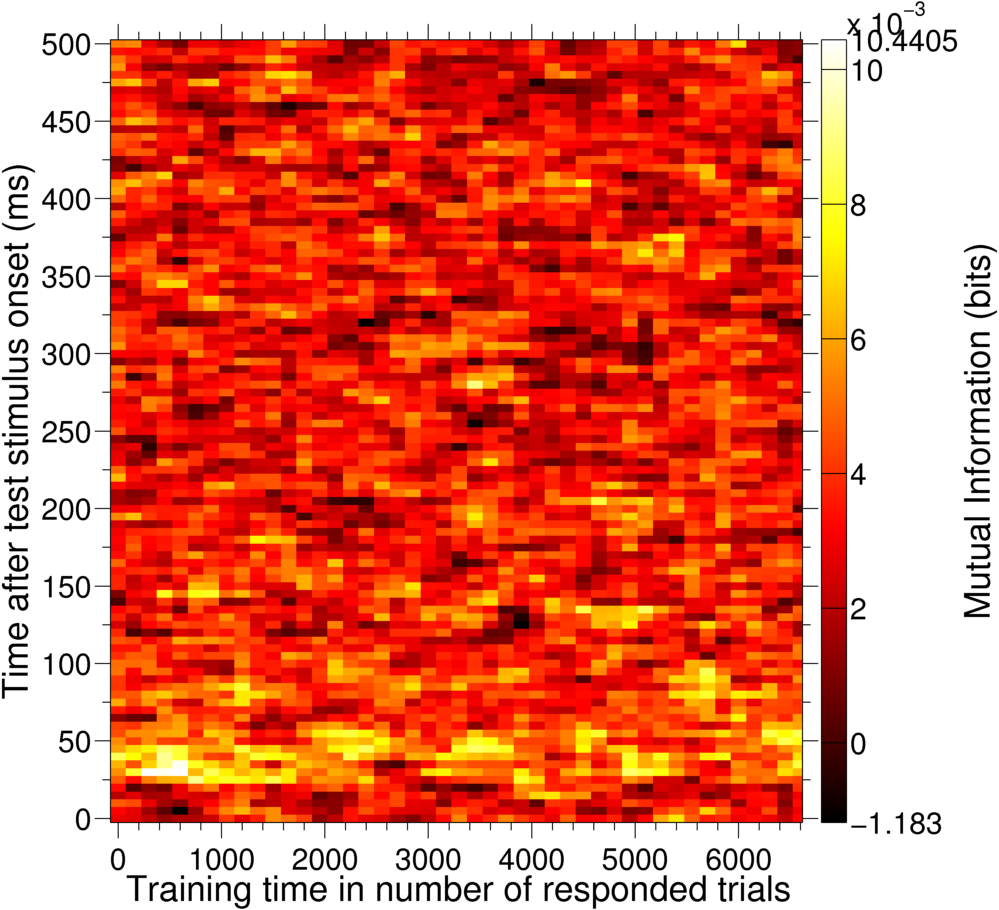
\includegraphics[scale=.25]{%
% % ./figs/I_trialwise_blanco_v1_chmean23_s343-354,355.1,355.2,356-359_tp4_1bins_of_20ms_dr_pt_oc0_test_tc22-3-28,32,35,40_nt600_ts150_rmvet1_rmvms1_pcolorhot_20120816T011920.png}
% %     \end{subfigure}
% %     ~~
% %     \begin{subfigure}[b]{0.5\linewidth}
% %         \centering
% %         \caption{}
% %         \label{fig:j1-1x20fc}
% %         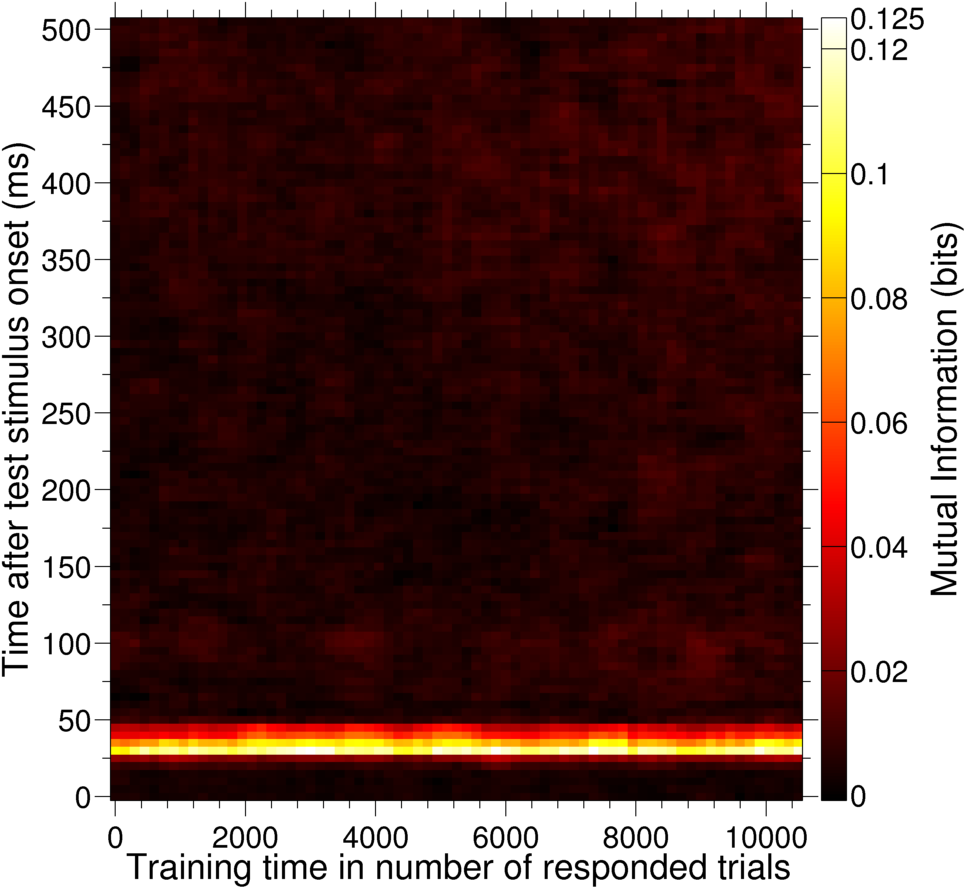
\includegraphics[scale=.25]{%
% % ./figs/I_trialwise_jack_v1_chmean25_s51-72_tp4_1bins_of_20ms_dr_pt_oc0_test_tc22-3-28,32,35,40_nt600_ts150_rmvet1_rmvms1_pcolorhot_20120816T011800.png}
% %     \end{subfigure}
% %     \caption{V1: Fine vs. coarse contrast differences.
% % % Mutual information between the test stimulus and \unit[20]{ms} of spiking activity.
% % % The PT bias correction method was used in all estimates of the information.
% % In the top panels, the six contrasts included are \{5, 15, 22, 40, 50, 90\}\%; bottom panels \{22, 25, 28, 32, 35, 40\}\%. An average of 100 trials per stimulus is used in each of these.
% % Left panels are for M1, right are M2.
% % In each case, mutual information between the six test stimuli and \unit[20]{ms} of spiking activity was measured using a spike count code, and bias corrected using the PT method.
% % % Panels \ref{fig:b1-1x20cc} and \ref{fig:b1-1x20fc} are for M1, \ref{fig:b1-1x20cc} and \ref{fig:b1-1x20fc} for M2.
% % }
% %     \label{fig:v1-fvc}
% % \end{figure}


% ./figs/I_trialwise_blanco_v4_chmean31_s307,308,311,313,314,317,318,320,321,329-341_tp4_1bins_of_20ms_dr_pt_oc0_test_tc10-5-20,40-10-60_nt600_ts150_rmvet1_rmvms1_pcolorhot_20120816T012120.png
% ./figs/I_trialwise_blanco_v4_chmean31_s307,308,311,313,314,317,318,320,321,329-341_tp4_1bins_of_20ms_dr_pt_oc0_test_tc27-29,31-33_nt600_ts150_rmvet1_rmvms1_pcolorhot_20120816T011952.png
% ./figs/I_trialwise_jack_v4_chmean20_s24-49_tp4_1bins_of_20ms_dr_pt_oc0_test_tc10-5-20,40-10-60_nt600_ts150_rmvet1_rmvms1_pcolorhot_20120816T011902.png
% ./figs/I_trialwise_jack_v4_chmean20_s24-49_tp4_1bins_of_20ms_dr_pt_oc0_test_tc27-29,31-33_nt600_ts150_rmvet1_rmvms1_pcolorhot_20120816T011843.png

% % \begin{figure}[htbp]
% %     \begin{subfigure}[b]{0.5\linewidth}
% %         \centering
% %         \caption{}
% %         \label{fig:b4-1x20cc}
% %         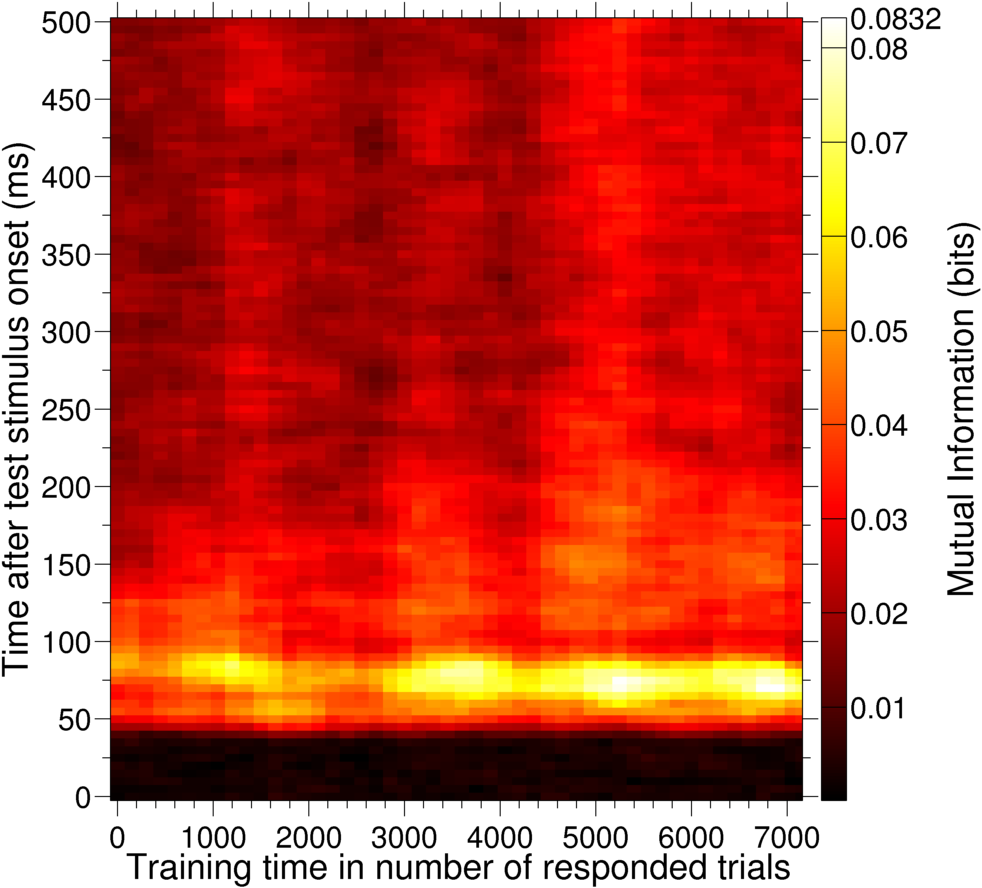
\includegraphics[scale=.25]{%
% % ./figs/I_trialwise_blanco_v4_chmean31_s307,308,311,313,314,317,318,320,321,329-341_tp4_1bins_of_20ms_dr_pt_oc0_test_tc10-5-20,40-10-60_nt600_ts150_rmvet1_rmvms1_pcolorhot_20120816T012120.png}
% %     \end{subfigure}
% %     ~~
% %     \begin{subfigure}[b]{0.5\linewidth}
% %         \centering
% %         \caption{}
% %         \label{fig:j4-1x20cc}
% %         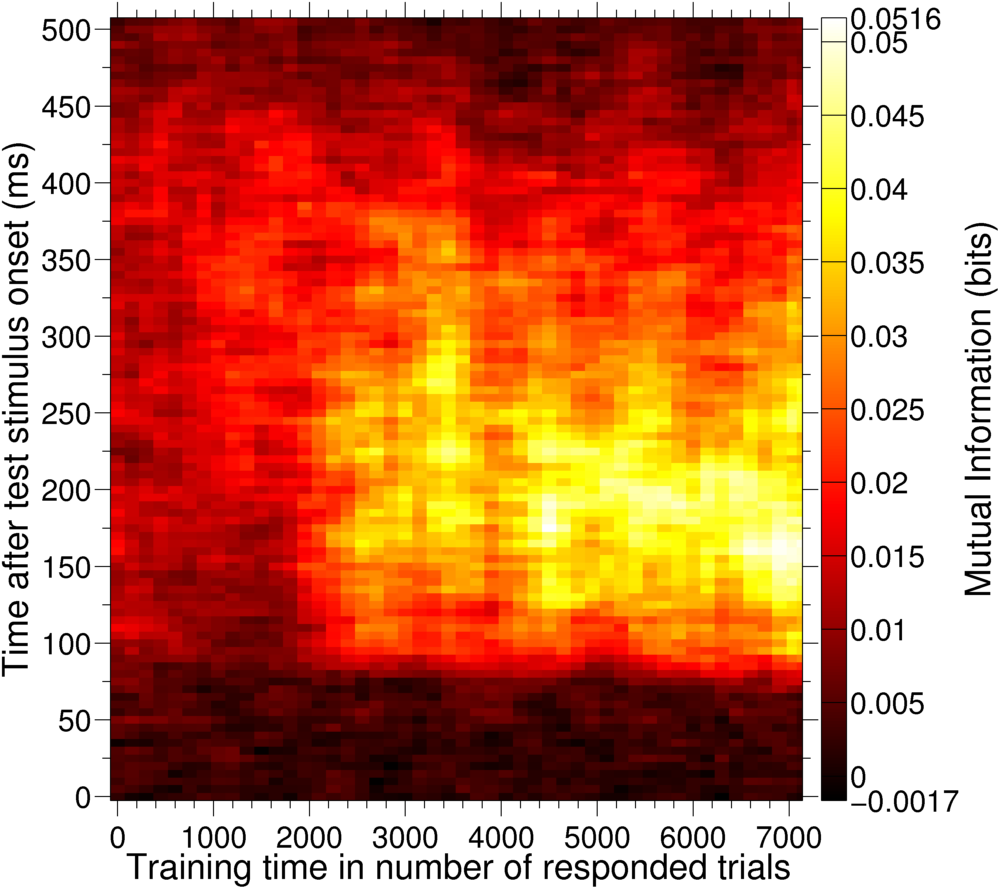
\includegraphics[scale=.25]{%
% % ./figs/I_trialwise_jack_v4_chmean20_s24-49_tp4_1bins_of_20ms_dr_pt_oc0_test_tc10-5-20,40-10-60_nt600_ts150_rmvet1_rmvms1_pcolorhot_20120816T011902.png}
% %     \end{subfigure}
% %     \\
% %     \begin{subfigure}[b]{0.5\linewidth}
% %         \centering
% %         \caption{}
% %         \label{fig:b4-1x20fc}
% %         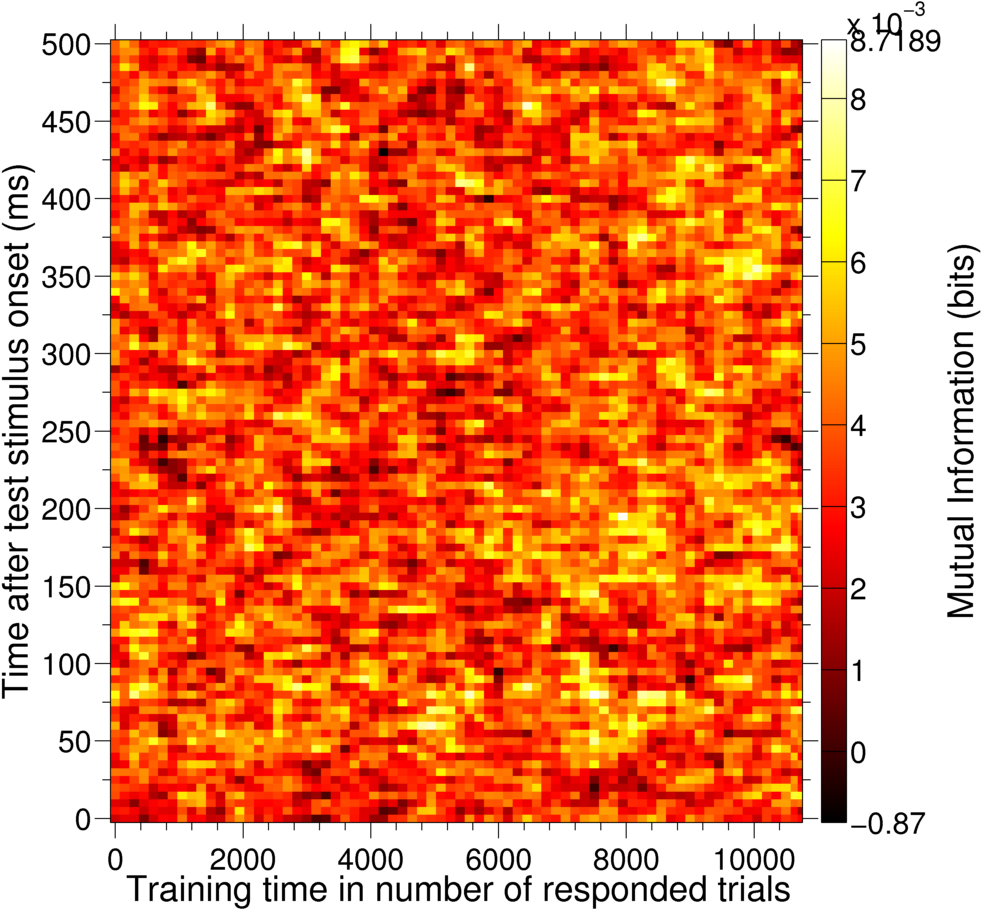
\includegraphics[scale=.25]{%
% % ./figs/I_trialwise_blanco_v4_chmean31_s307,308,311,313,314,317,318,320,321,329-341_tp4_1bins_of_20ms_dr_pt_oc0_test_tc27-29,31-33_nt600_ts150_rmvet1_rmvms1_pcolorhot_20120816T011952.png}
% %     \end{subfigure}
% %     ~~
% %     \begin{subfigure}[b]{0.5\linewidth}
% %         \centering
% %         \caption{}
% %         \label{fig:j4-1x20fc}
% %         \includegraphics[scale=.25]{%
% % ./figs/I_trialwise_jack_v4_chmean20_s24-49_tp4_1bins_of_20ms_dr_pt_oc0_test_tc27-29,31-33_nt600_ts150_rmvet1_rmvms1_pcolorhot_20120816T011843.png}
% %     \end{subfigure}
% %     \caption{V4: Fine vs coarse contrast differences.
% % % Mutual information between the test stimulus and \unit[20]{ms} of spiking activity.
% % % The PT bias correction method was used in all estimates of the information.
% % In the top panels, the six contrasts included are \{10, 15, 20, 40, 50, 60\}\%; bottom panels \{27, 28, 29, 31, 32, 33\}\%. An average of 100 trials per stimulus is used in each of these.
% % Left panels are for M1, right are M2.
% % In each case, mutual information between the six test stimuli and \unit[20]{ms} of spiking activity was measured using a spike count code, and bias corrected using the PT method.
% % % Panels \ref{fig:b1-1x20cc} and \ref{fig:b1-1x20fc} are for M1, \ref{fig:b1-1x20cc} and \ref{fig:b1-1x20fc} for M2.
% % }
% %     \label{fig:v4-fvc}
% % \end{figure}

For V4, we find there is no information about fine contrast differences in either animal (Figs.~\ref{fig:b4-1x20fc} and \ref{fig:j4-1x20fc}). The information about the coarse differences is higher than when all conditions are considered, for reasons discussed above, and these show the same trends as when we analysed all the conditions, in Figs.~\ref{fig:b4-1x20tp4} and \ref{fig:j4-1x20tp4}.

%----------------------------------------------------------------------------------------------------------------------
\FloatBarrier
\subsubsection{Information in millisecond-level spike timing}

For M2 V1, there seems to be some information in the millisecond-level timing of the spikes during the transient response, but not afterward this has elapsed (Fig.~\ref{fig:v1-dif}, right-hand panels). This band due to the transient is clearly well above the variance of the sampling for the rest of the window offsets.
However, the information in the transient is only present for the coarse contrasts and not for the fine contrasts.
For the fine contrast discrimination in M2 V1, shown in Fig.~\ref{fig:j1-fdif}, (and possibly to a lesser degree on a couple of the other figures) there is an unusual effect where there seems to be more information in the shuffled bins than the unshuffled bins.\footnote{When this is analysed for the raw data with the artifact included, this is subtly more prominently on several of the plots.}

For M1 V1, and also M1 V4, there seems to be an increase in the information contained in the spike timing during the transient also. However, these results are not as clear-cut as in M2 V1.

% ./figs/I_diff_trialwise_dur=20ms_nshuf=1_blanco_v1_chmean23_s343-354,355.1,355.2,356-359_tp4_dr_pt_oc0_test_tc5-5-20,22-3-28,32,35-5-50,60,90_nt1400_ts350_rmvet1_rmvms1_pcolorbp_20120816T010538.png
% ./figs/I_diff_trialwise_dur=20ms_nshuf=1_blanco_v1_chmean23_s343-354,355.1,355.2,356-359_tp4_dr_pt_oc0_test_tc5,15,22,40,50,90_nt600_ts150_rmvet1_rmvms1_pcolorbp_20120816T004933.png
% ./figs/I_diff_trialwise_dur=20ms_nshuf=1_blanco_v1_chmean23_s343-354,355.1,355.2,356-359_tp4_dr_pt_oc0_test_tc22-3-28,32,35,40_nt600_ts150_rmvet1_rmvms1_pcolorbp_20120816T004908.png
% 
% ./figs/I_diff_trialwise_dur=20ms_nshuf=1_jack_v1_chmean25_s51-72_tp4_dr_pt_oc0_test_tc5-5-20,22-3-28,32,35-5-50,60,90_nt1400_ts350_rmvet1_rmvms1_pcolorbp_20120816T004517.png
% ./figs/I_diff_trialwise_dur=20ms_nshuf=1_jack_v1_chmean25_s51-72_tp4_dr_pt_oc0_test_tc5,15,22,40,50,90_nt600_ts150_rmvet1_rmvms1_pcolorbp_20120816T010526.png
% ./figs/I_diff_trialwise_dur=20ms_nshuf=1_jack_v1_chmean25_s51-72_tp4_dr_pt_oc0_test_tc22-3-28,32,35,40_nt600_ts150_rmvet1_rmvms1_pcolorbp_20120816T004555.png

% % \begin{figure}[htbp]
% %     \begin{subfigure}[b]{0.5\linewidth}
% %         \centering
% %         \caption{}
% %         \label{fig:b1-alldif}
% %         \includegraphics[scale=.25]{%
% % ./figs/I_diff_trialwise_dur=20ms_nshuf=1_blanco_v1_chmean23_s343-354,355.1,355.2,356-359_tp4_dr_pt_oc0_test_tc5-5-20,22-3-28,32,35-5-50,60,90_nt1400_ts350_rmvet1_rmvms1_pcolorbp_20120816T010538.png}
% %     \end{subfigure}
% %     ~~
% %     \begin{subfigure}[b]{0.5\linewidth}
% %         \centering
% %         \caption{}
% %         \label{fig:j1-alldif}
% %         \includegraphics[scale=.25]{%
% % ./figs/I_diff_trialwise_dur=20ms_nshuf=1_jack_v1_chmean25_s51-72_tp4_dr_pt_oc0_test_tc5-5-20,22-3-28,32,35-5-50,60,90_nt1400_ts350_rmvet1_rmvms1_pcolorbp_20120816T004517.png}
% %     \end{subfigure}
% %     \\
% %     \begin{subfigure}[b]{0.5\linewidth}
% %         \centering
% %         \caption{}
% %         \label{fig:b1-cdif}
% %         \includegraphics[scale=.25]{%
% % ./figs/I_diff_trialwise_dur=20ms_nshuf=1_blanco_v1_chmean23_s343-354,355.1,355.2,356-359_tp4_dr_pt_oc0_test_tc5,15,22,40,50,90_nt600_ts150_rmvet1_rmvms1_pcolorbp_20120816T004933.png}
% %     \end{subfigure}
% %     ~~
% %     \begin{subfigure}[b]{0.5\linewidth}
% %         \centering
% %         \caption{}
% %         \label{fig:j1-cdif}
% %         \includegraphics[scale=.25]{%
% % ./figs/I_diff_trialwise_dur=20ms_nshuf=1_jack_v1_chmean25_s51-72_tp4_dr_pt_oc0_test_tc5,15,22,40,50,90_nt600_ts150_rmvet1_rmvms1_pcolorbp_20120816T010526.png}
% %     \end{subfigure}
% %     \\
% %     \begin{subfigure}[b]{0.5\linewidth}
% %         \centering
% %         \caption{}
% %         \label{fig:b1-fdif}
% %         \includegraphics[scale=.25]{%
% % ./figs/I_diff_trialwise_dur=20ms_nshuf=1_blanco_v1_chmean23_s343-354,355.1,355.2,356-359_tp4_dr_pt_oc0_test_tc22-3-28,32,35,40_nt600_ts150_rmvet1_rmvms1_pcolorbp_20120816T004908.png}
% %     \end{subfigure}
% %     ~~
% %     \begin{subfigure}[b]{0.5\linewidth}
% %         \centering
% %         \caption{}
% %         \label{fig:j1-fdif}
% %         \includegraphics[scale=.25]{%
% % ./figs/I_diff_trialwise_dur=20ms_nshuf=1_jack_v1_chmean25_s51-72_tp4_dr_pt_oc0_test_tc22-3-28,32,35,40_nt600_ts150_rmvet1_rmvms1_pcolorbp_20120816T004555.png}
% %     \end{subfigure}
% %     \caption{V1: Information in millisecond level spike timing.
% % % Mutual information between the test stimulus and \unit[20]{ms} of spiking activity.
% % % The PT bias correction method was used in all estimates of the information.
% % The information with time-wise shuffled bins was subtracted from information in the spike time code with a \unit[20]{ms} window subdivided into 5 bins.
% % Information was bias corrected using the PT method.
% % Left panels: M1; Right: M2.
% % Top panels: all contrasts, \{10, 15, 20, 25, 27, 28, 29, 31, 32, 33, 35, 40, 50, 60\}\%.
% % Centre panels: \{5, 15, 22, 40, 50, 90\}\%.
% % Bottom panels: \{22, 25, 28, 32, 35, 40\}\%.
% % An average of 100 trials per stimulus is used in the analysis for each.
% % % Panels \ref{fig:b1-1x20cc} and \ref{fig:b1-1x20fc} are for M1, \ref{fig:b1-1x20cc} and \ref{fig:b1-1x20fc} for M2.
% % }
% %     \label{fig:v1-dif}
% % \end{figure}


% ./figs/I_diff_trialwise_dur=20ms_nshuf=1_blanco_v4_chmean31_s307,308,311,313,314,317,318,320,321,329-341_tp4_dr_pt_oc0_test_tc10-5-20,40-10-60_nt600_ts150_rmvet1_rmvms1_pcolorbp_20120816T011506.png
% ./figs/I_diff_trialwise_dur=20ms_nshuf=1_blanco_v4_chmean31_s307,308,311,313,314,317,318,320,321,329-341_tp4_dr_pt_oc0_test_tc10-5-25,27-29,31-33,35,40-10-60_nt1400_ts350_rmvet1_rmvms1_pcolorbp_20120816T004958.png
% ./figs/I_diff_trialwise_dur=20ms_nshuf=1_blanco_v4_chmean31_s307,308,311,313,314,317,318,320,321,329-341_tp4_dr_pt_oc0_test_tc27-29,31-33_nt600_ts150_rmvet1_rmvms1_pcolorbp_20120816T005048.png
% 
% ./figs/I_diff_trialwise_dur=20ms_nshuf=1_jack_v4_chmean20_s24-49_tp4_dr_pt_oc0_test_tc10-5-20,40-10-60_nt600_ts150_rmvet1_rmvms1_pcolorbp_20120816T213446.png
% ./figs/I_diff_trialwise_dur=20ms_nshuf=1_jack_v4_chmean20_s24-49_tp4_dr_pt_oc0_test_tc10-5-25,27-29,31-33,35,40-10-60_nt1400_ts350_rmvet1_rmvms1_pcolorbp_20120816T004709.png
% ./figs/I_diff_trialwise_dur=20ms_nshuf=1_jack_v4_chmean20_s24-49_tp4_dr_pt_oc0_test_tc27-29,31-33_nt600_ts150_rmvet1_rmvms1_pcolorbp_20120816T004741.png

% % \begin{figure}[htbp]
% %     \begin{subfigure}[b]{0.5\linewidth}
% %         \centering
% %         \caption{}
% %         \label{fig:b4-alldif}
% %         \includegraphics[scale=.25]{%
% % ./figs/I_diff_trialwise_dur=20ms_nshuf=1_blanco_v4_chmean31_s307,308,311,313,314,317,318,320,321,329-341_tp4_dr_pt_oc0_test_tc10-5-25,27-29,31-33,35,40-10-60_nt1400_ts350_rmvet1_rmvms1_pcolorbp_20120816T004958.png}
% %     \end{subfigure}
% %     ~~
% %     \begin{subfigure}[b]{0.5\linewidth}
% %         \centering
% %         \caption{}
% %         \label{fig:j4-alldif}
% %         \includegraphics[scale=.25]{%
% % ./figs/I_diff_trialwise_dur=20ms_nshuf=1_jack_v4_chmean20_s24-49_tp4_dr_pt_oc0_test_tc10-5-25,27-29,31-33,35,40-10-60_nt1400_ts350_rmvet1_rmvms1_pcolorbp_20120816T004709.png}
% %     \end{subfigure}
% %     \\
% %     \begin{subfigure}[b]{0.5\linewidth}
% %         \centering
% %         \caption{}
% %         \label{fig:b4-cdif}
% %         \includegraphics[scale=.25]{%
% % ./figs/I_diff_trialwise_dur=20ms_nshuf=1_blanco_v4_chmean31_s307,308,311,313,314,317,318,320,321,329-341_tp4_dr_pt_oc0_test_tc10-5-20,40-10-60_nt600_ts150_rmvet1_rmvms1_pcolorbp_20120816T011506.png}
% %     \end{subfigure}
% %     ~~
% %     \begin{subfigure}[b]{0.5\linewidth}
% %         \centering
% %         \caption{}
% %         \label{fig:j4-cdif}
% %         \includegraphics[scale=.25]{%
% % ./figs/I_diff_trialwise_dur=20ms_nshuf=1_jack_v4_chmean20_s24-49_tp4_dr_pt_oc0_test_tc10-5-20,40-10-60_nt600_ts150_rmvet1_rmvms1_pcolorbp_20120816T213446.png}
% %     \end{subfigure}
% %     \\
% %     \begin{subfigure}[b]{0.5\linewidth}
% %         \centering
% %         \caption{}
% %         \label{fig:b4-fdif}
% %         \includegraphics[scale=.25]{%
% % ./figs/I_diff_trialwise_dur=20ms_nshuf=1_blanco_v4_chmean31_s307,308,311,313,314,317,318,320,321,329-341_tp4_dr_pt_oc0_test_tc27-29,31-33_nt600_ts150_rmvet1_rmvms1_pcolorbp_20120816T005048.png}
% %     \end{subfigure}
% %     ~~
% %     \begin{subfigure}[b]{0.5\linewidth}
% %         \centering
% %         \caption{}
% %         \label{fig:j4-fdif}
% %         \includegraphics[scale=.25]{%
% % ./figs/I_diff_trialwise_dur=20ms_nshuf=1_jack_v4_chmean20_s24-49_tp4_dr_pt_oc0_test_tc27-29,31-33_nt600_ts150_rmvet1_rmvms1_pcolorbp_20120816T004741.png}
% %     \end{subfigure}
% %     \caption{V4: Information in millisecond level spike timing.
% % % Mutual information between the test stimulus and \unit[20]{ms} of spiking activity.
% % % The PT bias correction method was used in all estimates of the information.
% % The information with time-wise shuffled bins was subtracted from information in the spike time code with a \unit[20]{ms} window subdivided into 5 bins.
% % Information was bias corrected using the PT method.
% % Left panels: M1; Right: M2.
% % Top panels: all contrasts, \{5, 10, 15, 20, 22, 25, 28, 32, 35, 40, 45, 50, 60, 90\}\%.
% % Centre panels: \{10, 15, 20, 40, 50, 60\}\%.
% % Bottom panels: \{27, 28, 29, 31, 32, 33\}\%.
% % An average of 100 trials per stimulus is used in the analysis for each.
% % % Panels \ref{fig:b1-1x20cc} and \ref{fig:b1-1x20fc} are for M1, \ref{fig:b1-1x20cc} and \ref{fig:b1-1x20fc} for M2.
% % }
% %     \label{fig:v4-dif}
% % \end{figure}


For M2 V4, there is no information in the spike timing measured on the millisecond timescale: not even during the transient response.

For any of these figures there certainly does not seem to be any change in the information contained in the spike timing alone, so it does not seem to be a trait which can be learned.

% This is true even if we only consider fine contrast differences as well, refuting our hypothesis that there will be more information in the spike timing for more finely differing stimuli contrasts.
% 
% %----------------------------------------------------------------------------------------------------------------------
% %----------------------------------------------------------------------------------------------------------------------
% %----------------------------------------------------------------------------------------------------------------------
% \chapter{$d'$ Analysis}
% %----------------------------------------------------------------------------------------------------------------------
% 
% In an attempt to clean up the data and only use the channels and sessions which provide the most relevant results
% 
% Discriminating based on the information content in the channels would allow us to ``cherry-pick'' the best data and artificially inflate the results, so an independent metric of data quality was sought. Since we are interested in the channels where the data is of reasonable quality and the neurons represented by the channel are responsive to the stimulus, $d'$ was used.
% 
% $d'$ is ...
% 
% %----------------------------------------------------------------------------------------------------------------------
% \subsection{Methods}
% 
% % How is it computed?
% 
% % $$
% % \mu_{stim} = mean(a_{stim});
% % \mu_{spon} = mean(a_{spon});
% % 
% % % Combine the standard deviations of the two sets of trials
% % % Have to do a weighted average of the variances
% % stdev_joint = sqrt(...
% %     ( (n_stim-1)*var(act_stim) + (n_spon-1)*var(act_spon) ) ...
% %     / (n_stim + n_spon - 2) ...
% %     );
% 
% $$
% d\,' = \frac{\mu_{stim} - \mu_{spon}}{\sigma_{joint}}
% ,$$
% where the joint standard deviation over both populations is given by 
% $$
% \sigma_{joint} = \sqrt
%     \frac{ (n_{stim}-1) \, \sigma_{stim} + (n_{spon}-1) \, \sigma_{spon} }
%     { n_{stim} + n_{spon} - 2}
% $$
% so that it is weighted by the number of datapoints, $n_{stim}$ and $n_{spon}$, for both the stimulus presentation and spontaneous activity 
% 
% References
% Compared the mean firing rate for spontaneous activity and the sample stimulus of 30\% contrast
% Compared the mean firing rate for spontaneous activity and the highest contrast test stimulus
% 
% %----------------------------------------------------------------------------------------------------------------------
% \subsection{Results}
% 
% d' increases with learning
% 
% Just using channels with a session-wise mean d' > X gives us cleaner results

%----------------------------------------------------------------------------------------------------------------------
\chapter{Discussions}

We now discuss the findings of the analysis described in the previous chapter, and suggest ways in which this work may proceed in the future.

%----------------------------------------------------------------------------------------------------------------------
\section{Validity of results}

From Figs.~\ref{fig:b1-trialwise}--\ref{fig:j4-trialwise}, we can conclude several things about the reliability of our other results.
Firstly, it seems the data for M2 is more trustworthy than that of M1.
Secondly, from the information measured in the spontaneous activity, it seems the results for the spike timing code cannot be trusted, certainly not any changes which seem to occur with learning.
Thirdly, this latter point may call into jeopardy the reliability of the results for the spike count code, since these problems seem to be inherent to the raw data, though the information in the spike count code is more robust due to its fewer possible response vectors.

%----------------------------------------------------------------------------------------------------------------------
\section{Discussion of results}

The analysis has demonstrated there is far more information given by the onset transient response, which is in keeping with previous findings \cite{Muller2001}.

The finding that information increases more rapidly with learning in V4 than V1 is in line with our hypothesis made earlier.

The result that the peak in information in V4 neurons moves to being sooner after stimulus onset (Fig.~\ref{fig:j4-1x20tp4}) is an entirely novel finding. Although the values for the information here are very low --- only \unit[0.02]{bits} --- this is the average over many channels, only a couple of which exhibit the increase with time. The more responsive channels have information peaking at around \unit[0.65]{bits}, but the non-responsive channels pull this average down. I have also done some work to identify which channels should be excluded on the basis of their $d'$, but this is not presented here.

%----------------------------------------------------------------------------------------------------------------------
\section{Fine versus coarse contrast differences}

We did not find that learning was focused on the more difficult contrasts with the fine differences between them. If there is an increase in the information in V1, it is not very large and occurs for all groups of contrasts to the same degree. Curiously, for V4, it seems that the neurons improve their discriminability for the coarsely differentiated contrasts, but not the fine differences, which is the opposite to what was anticipated. It could be that fine stimuli differences cannot be accurately resolved using the signals from only individual neurons, and concurrent signals from a population of neurons are needed for this to be finer discrimination to be possible.

%----------------------------------------------------------------------------------------------------------------------
\section{Information in millisecond-level spike timing}

The observation about there being more information in the shuffled timebins than when they are in their genuine order (Fig.~\ref{fig:j1-fdif}) should be an impossibility because shuffling the response bins around can only destroy information and cannot generate it as it is a random process, unrelated to the stimuli.
This could, however, be explained if spikes are similarly timed in the actual data for many stimuli, which causes their responses to be more similar than one would expect by chance. In this case, there might be reliably more information measured in the shuffled bins due to the bias of the measurement being higher when the responses are less predictable.

The information in the precise spike timing for V1 would fit with previous results which have suggested there is information in the latency of the onset response
\cite{Reich2001,Tovee1993,Rolls2011}.
Moreover, \cite{Tovee1993,Rolls2011} indicates that for the primary visual cortex there is no information in the spike-timing beyond that of the spike code except for the limited amount of information given in the latency.
In addition, the work presented here suggests that although the latency of the response in V1 conveys information about the presented contrast, this is not a learned or learnable trait.


It was not found that there is more information contained in the spike timing for finer contrast differences. This is contrary to the initial hypothesis, and contradicts several existing pieces of research \cite{Reich2001,Arabzadeh2006}, but it corroborates the items of research just mentioned indicating there is no information in spike-timing beyond the response latency \cite{Reich2001,Tovee1993,Rolls2011}.
As the bodies of work suggesting there would be differences for fine and coarse discrimination were based on recordings in the rat somatosensory system, whilst the latter is based in the visual cortex, this is not too surprising.
However, as we have already stated, any results from our analysis on spike timing codes are questionable due to the our control of the information in the spontaneous activity.

%----------------------------------------------------------------------------------------------------------------------
\section{Future Work}

Further work will need to be done on this analysis to try and fix the inconsistencies in data between days so they can be studied together more easily. Also, work will need to be done to establish if any of the results presented here are genuinely statistically significant.

Here we describe some follow-up work which could be performed, either by myself or the perceptual learning lab group.

%----------------------------------------------------------------------------------------------------------------------
\subsection{Elimination of artifacts from continuous data}

Fig.~\ref{fig:mahist-j1s56} shows that the current method of correcting for the monitor artifact is flawed.
If the monitor artifact were an artifact similar to previously known artifacts, such as the ``reward artifact'' generated by the water dispenser, a large potential is induced in the electrode, which can be registered as a spike since it exceeds the threshold. However, this sort of behaviour would not cause a reduction in the number of spikes preceding the artifact incident, as seen here and in many of the sessions for other channels too.

To create the preceding reduction in spikes over a period of around \unit[0.2]{ms}, the measured potential must be reduced, suppressing the spikes which are being elicited so they are not passing threshold and being detected.
A positive electric potential following this could increase the proportion of spikes meeting threshold, and resulting in the problematic sharp peak in the number of spikes.
Lending credence to this theory is the way the spikes detected as the monitor artifact have the same waveform as the usual spike, but have an amplitude towards the lower end of what would be expected.

If this is the effect we are witnessing, this can be fixed in a manner similar to the way the monitor artifacts were removed in this paper. Instead of considering the spiking data, we will need to look at the continuous data. We can take the modulo of the times with respect to the monitor refresh rate again, and bin the datapoints together with a bin width the reciprocal of the sampling frequency, but instead of taking the number of datapoints in each bin (which will be the same since there is always a continuous voltage value even if there isn't a spike), we take the mean of the voltages. The amount of modification made on each trial to the voltages should then appear as a fluctuation in the mean voltage recorded and can consequently be subtracted from the original data.

%----------------------------------------------------------------------------------------------------------------------
\subsection{Normalisation of firing rates}

Combining trials from different sessions in one analysis has problems because the recording quality varies from day to day.
Can possibly be normalised by adjusting the spike detection threshold so that there is always the same spontaneous activity exceeding the threshold
This is justifiable because even if neuronal firing rates change greatly due to perceptual learning, homeostasis should keep the spontaneous activity rates relatively consistent.

This will hopefully make the measured information content of the spontaneous activity be consistent throughout training. If this is the case, the result will be much more trustworthy results. This will be especially important in improving the potential of the results for M1, and for the spike-timing code, potentially yielding some more interesting results.

%----------------------------------------------------------------------------------------------------------------------
\subsection{Comparison with pyschometrics}

An interesting comparison would be to see how the information correlates with the behaviour of the monkey.
In particular, it is suspected that there might be a correlation between the magnitude of the maximum information available to the animal in V4 and the performance of the monkey in the task.
Also, there is reason to suspect there might be a correlation between the latency of the information in V4 and the response time of the monkey, and I tentatively hypothesise this will be the case.

%----------------------------------------------------------------------------------------------------------------------
\subsection{Statistical analysis of significance of results}

It will be very important to clarify the statistical significance, if any, of the results tentatively presented here.
The statistical significance of mutual information can be estimated by using bootstrapping, which is where the stimuli and response vectors are shuffled and paired together at random \cite{Ince2011}. Because some combinations will happen to provide more discriminability than others, the distributed of the mutual information fits a Gaussian distribution with a certain mean and standard deviation. By taking the distribution of information with bootstrapping, the mean and variance can be computed, and the actual value of the information from the data can be compared with this to see if its distance above the mean is statistically significant.

Using this method, we can also pick out a value of information which is statistically significant and see how long after test presentation it takes for the information about the test stimulus to become significant. This will provide a metric for information latency.

%----------------------------------------------------------------------------------------------------------------------
\subsection{Further directions}

There are several different routes down which the project could be more broadly extended.

\begin{itemize}
\item Analysis of information about the test contrast contained in the MUA and LFP signals contained in the raw recordings from which the spiking data was extracted.
\item Analysis of roving task. This could be done by considering the activity during test presentation identifying the trial condition as being dependent on both test and sample contrasts. To see how important the sample stimulus is to the brain activity during the test presentation, we would subtract from this an estimate of the information where condition is changed by keeping the test contrasts the same, but shuffling the sample contrasts.
\item Information rate in bits per spike \cite{Rolls2011}.
\item Population wide information, using a decoding approach. There are too many channels to use a direct information theoretic approach \cite{Quiroga2009}.
If we were to use information theory directly, even with binary bins for every channel, there are $2^20$ possible responses and we would need in excess of 2 million trials per condition to have a reasonable estimate of the information content. The dataset is not large enough for this, and even if it were we would have missed the changes due to perceptual learning as they only occur in the first 20,000 trials.
\item Examining correlations between neurons.
\item Investigate whether firing rate for different contrasts becomes more discriminable due to the means becoming more distant or due to the variability in rate for each contrast being reduced.
\end{itemize}

% 
% %----------------------------------------------------------------------------------------------------------------------
\section{Summary}

The project has expanded on existing literature and demonstrated that the millisecond-level timing of spikes from individual neurons, both in V1 and V4, is not important for contrast discrimination tasks, but the firing rate is important. It has also been demonstrated that little information regarding the discrimination between similar contrasts can be gained from the spiking activity of individual neurons, even during/after perceptual learning has occurred. In V1, there is no discernible change in contrast information in individual neurons at all, but in V4 there is an increase with perceptual learning in the magnitude of the peak information after stimulus onset, and the peak occurs sooner after stimulus onset as well.

However, the analysis indicates the quality of the results is good for one monkey (M2), but not so good for the other (M1). The discrepancy between the two datasets needs further investigation, and the conclusions made here need to be validated against other studies.

%
%
%%%%%%%%
%% Any appendices should go here. The appendix files should look just like the
%% chapter files.
\appendix
% \include{appendix1}
%
%
%\addcontentsline{toc}{chapter}{\numberline{}Bibliography}
%
%% Choose your favourite bibliography style here.
% \bibliographystyle{apalike}
\bibliographystyle{ieeetr}  % plain, ieeetr
%
\bibliography{summer.bib,summer_custom.bib}
%
%
\end{document}
%
%----------------------------------------------------------------------------------------------------------------------
